\chapter{Signal and background modelling}
\label{chap:model}

The statistical interpretation of the data requires models of the expected \mgg distribution for the signal and background processes in each category. These models must account for the sources of systematic uncertainty which affect the analysis. %The signal here refers to the diphoton events produced by one of the main Higgs production processes \ggH, \VBF, \ttH, and \VH, where the latter can be further split into \WH and \ZH. 
For the signal processes, the \mgg distribution takes the form of a resonant peak around \mH, the width of which is entirely dominated by detector resolution. The construction of the signal model is described in \Sec~\ref{model:sec:signal_model}. By contrast, the \mgg distribution for background events is a falling non-resonant continuum. The method by which the background model is produced from data is described in \Sec~\ref{model:sec:background_model}. Finally, the handling of the systematic uncertainties is described in \Sec~\ref{model:sec:systematics}. 

\section{Signal modelling}
\label{model:sec:signal_model}

\subsection{Parametrisation of the signal \mgg distributions}

%A signal model is constructed from samples of simulated \Hgg events from each production mode. . % are reconstructed, selected and categorised as described in Chapters~\ref{} and ~\ref{}. 
The shape of the \mgg distribution is parametrised separately for each event category and production process, where the \VH events are further split into \WH and \ZH samples. Since the vertex choice affects the shape of the \mgg  distribution, as was mentioned in \Sec~\ref{reco:sec:vertex}, the modelling is performed separately for cases where the \RV or \WV  was selected. 

The signal \mgg distributions are all parametrised using a \DCB function~\cite{CrystalBallFunction} summed with an additional Gaussian function sharing the same mean. We refer to this functional form hereafter as a \DCBpG function. %The \CB functional form is used in \HEP to model processes which involve losses, for example in the semiparmetric regression described in Sec~\ref{}, where it is used to model the energy of individual photons. 
The \DCB shape consists of a Gaussian function core and two tails which are described by power laws. The Gaussian core models the width of the distribution, while the power laws cover the extended non-Gaussian tails caused by systematic under- or over-estimation of the value of \mgg. %For example, the \DCB shape is used iin the semiparmetric regression described in \Sec~\ref{} to model photon energy distribution. The lower tail captures the fact that a certain amount of energy of the photon can be lost in the reconstruction process, this leading to a long non-Gaussian tail of events. Ont he other side, the upper tailis motivated theenergy of the photon shower can be over-estimated, for example because of the inclsuio of showers due to \PU.  
The \DCB shape has five parameters: the width and mean of the Gaussian core, the cross-over points to the power laws on each side, and the order of the two power laws. The \DCBpG function therefore has a total of seven parameters. This is in contrast with the functional form used for signal modelling in previous studies of \Hgg at \CMS~\cite{LegacyHgg,CMS-PAS-HIG-15-005,CMS-PAS-HIG-16-020}, which was a sum of up to five Gaussian functions, or a total of up to fourteen parameters.

The values of the parameters of the functional form are determined using a \NLL minimisation to fit the simulated \mgg distributions.
The choice of the \DCBpG function is motivated by the fact that it gives closer agreement than the simple sum of Gaussian functions, with substantially fewer degrees of freedom. The \DCB shape is also better motivated physically than an arbitrary sum of Gaussian functions. 

The parametrisations of the \mgg distributions for the \ggH process (with $\mH=125\GeV$) in the inclusive categories are shown in \Fig~\ref{fig:model:functionalform} for both the \DCBpG and sum of Gaussians functional forms. The improvement in the agreement between the distribution and the parametrisation can be quantified by comparing the $\chi^2$ values and the number of degrees of freedom. The \DCBpG typically gives a better agreement and this is also true for the other processes and categories.

\begin{figure}[ht!]
\centering
  \subfloat[Functional form: DCB$+1$G]{\shortstack{
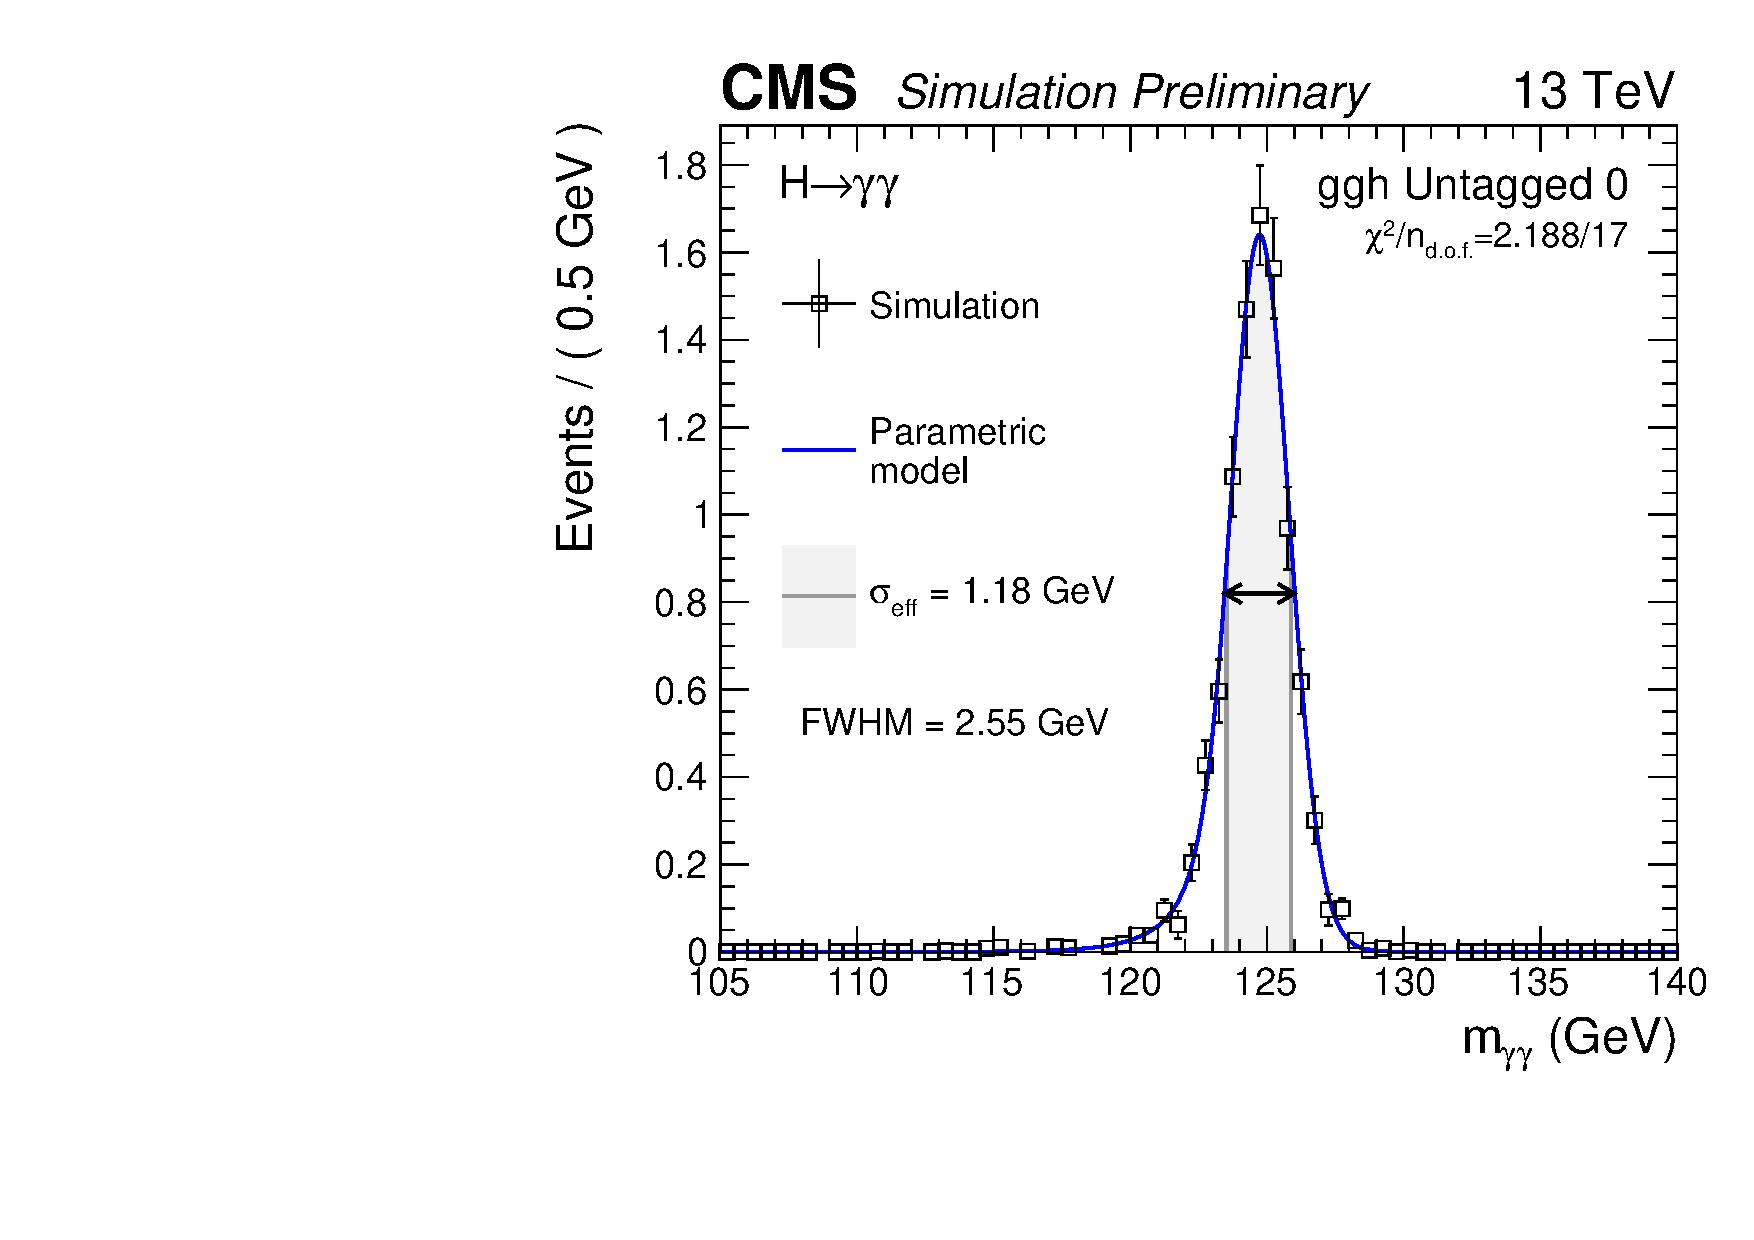
\includegraphics[width=0.3\textwidth]{modellingFigures/DCBpG/ggh_UntaggedTag_0.pdf} 
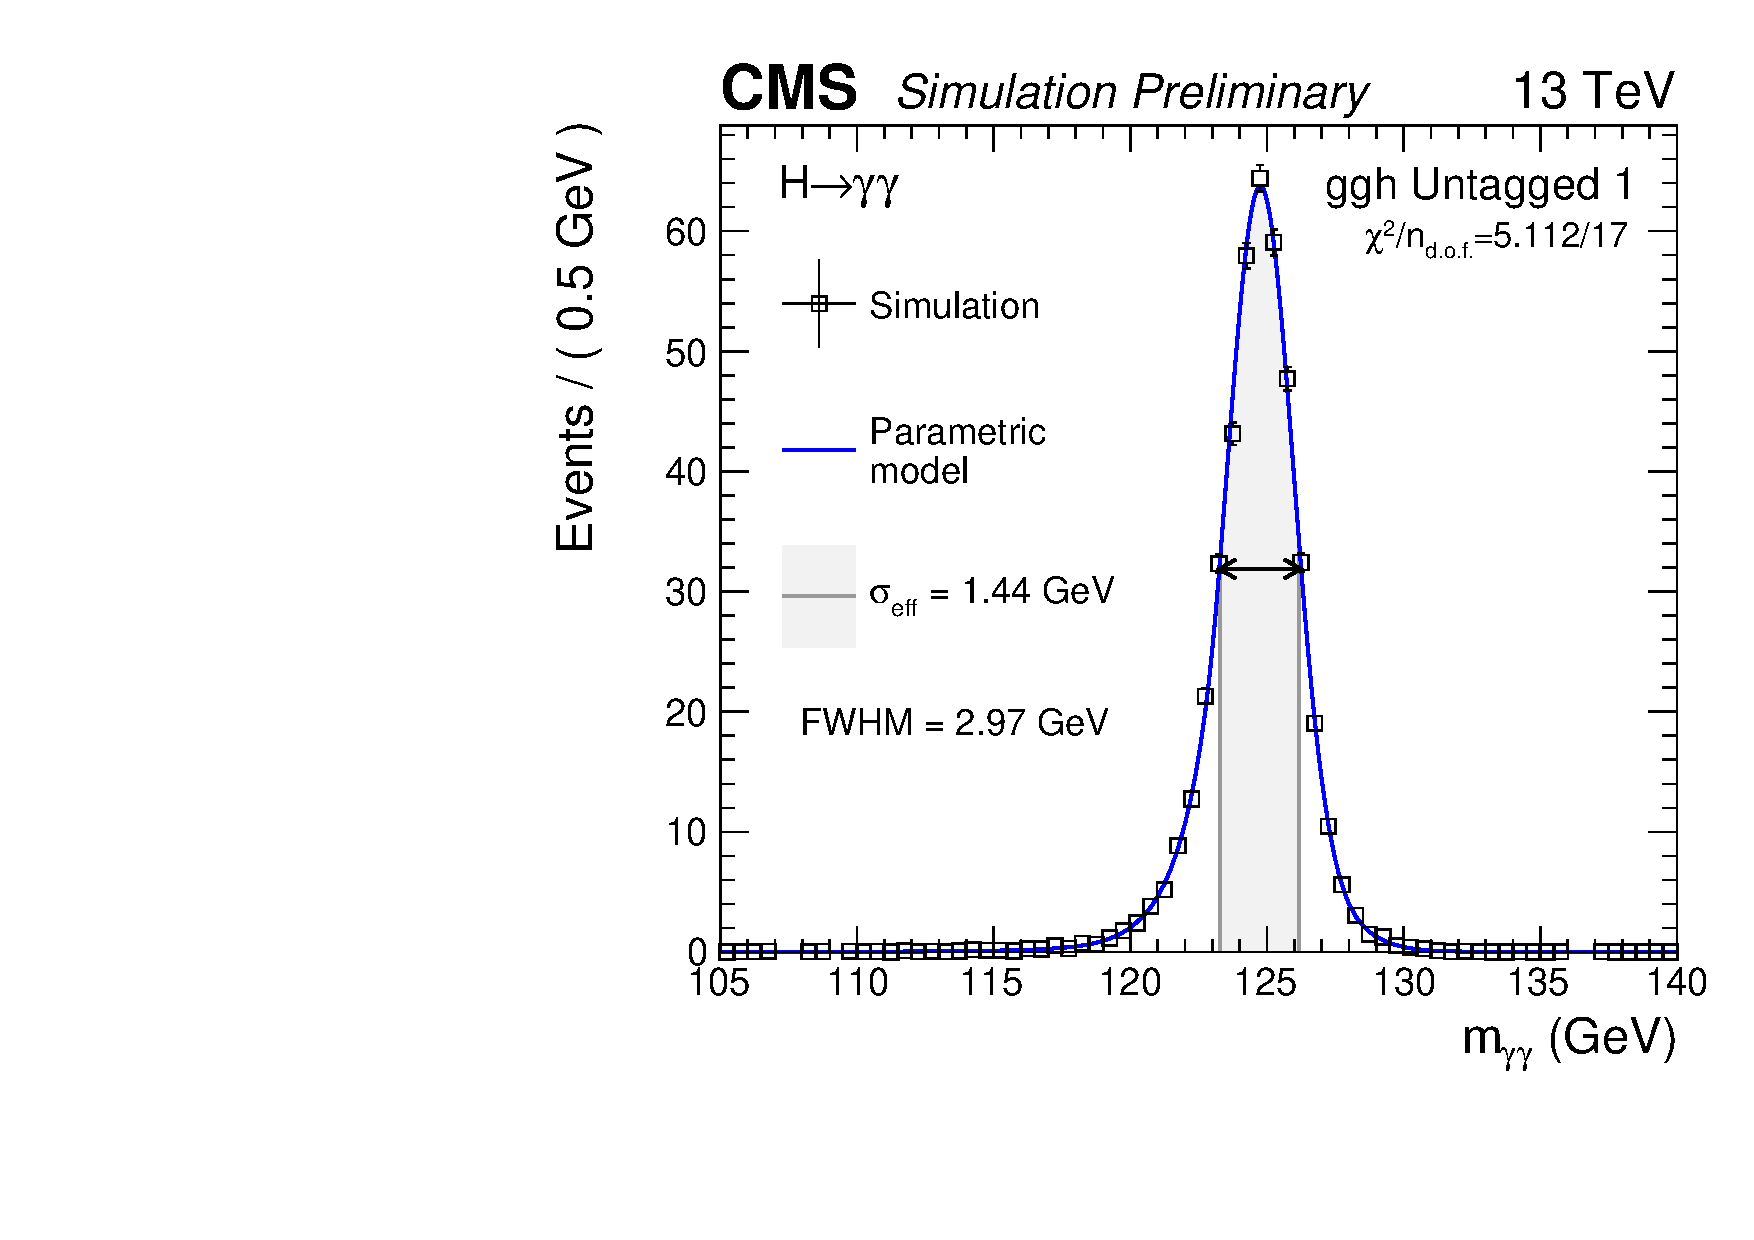
\includegraphics[width=0.3\textwidth]{modellingFigures/DCBpG/ggh_UntaggedTag_1.pdf} \\
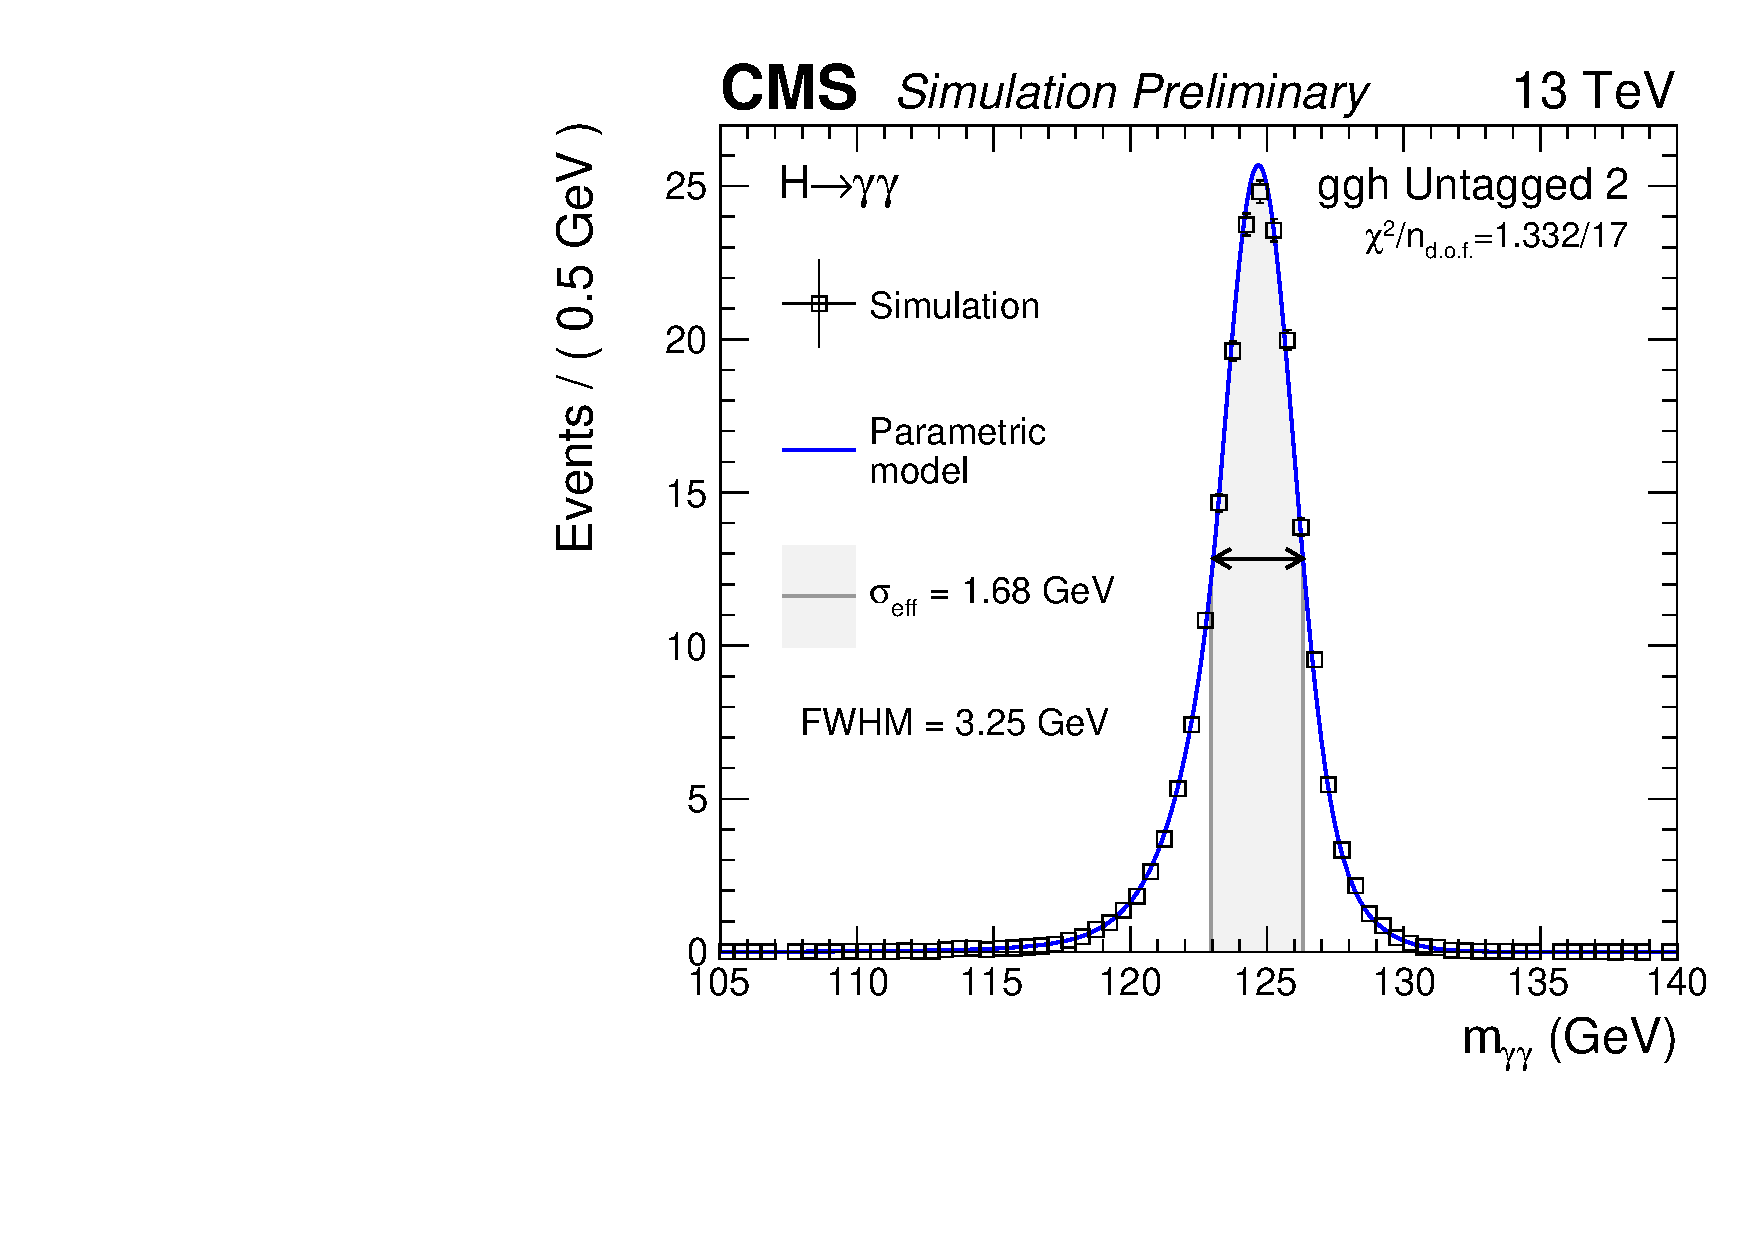
\includegraphics[width=0.3\textwidth]{modellingFigures/DCBpG/ggh_UntaggedTag_2.pdf} 
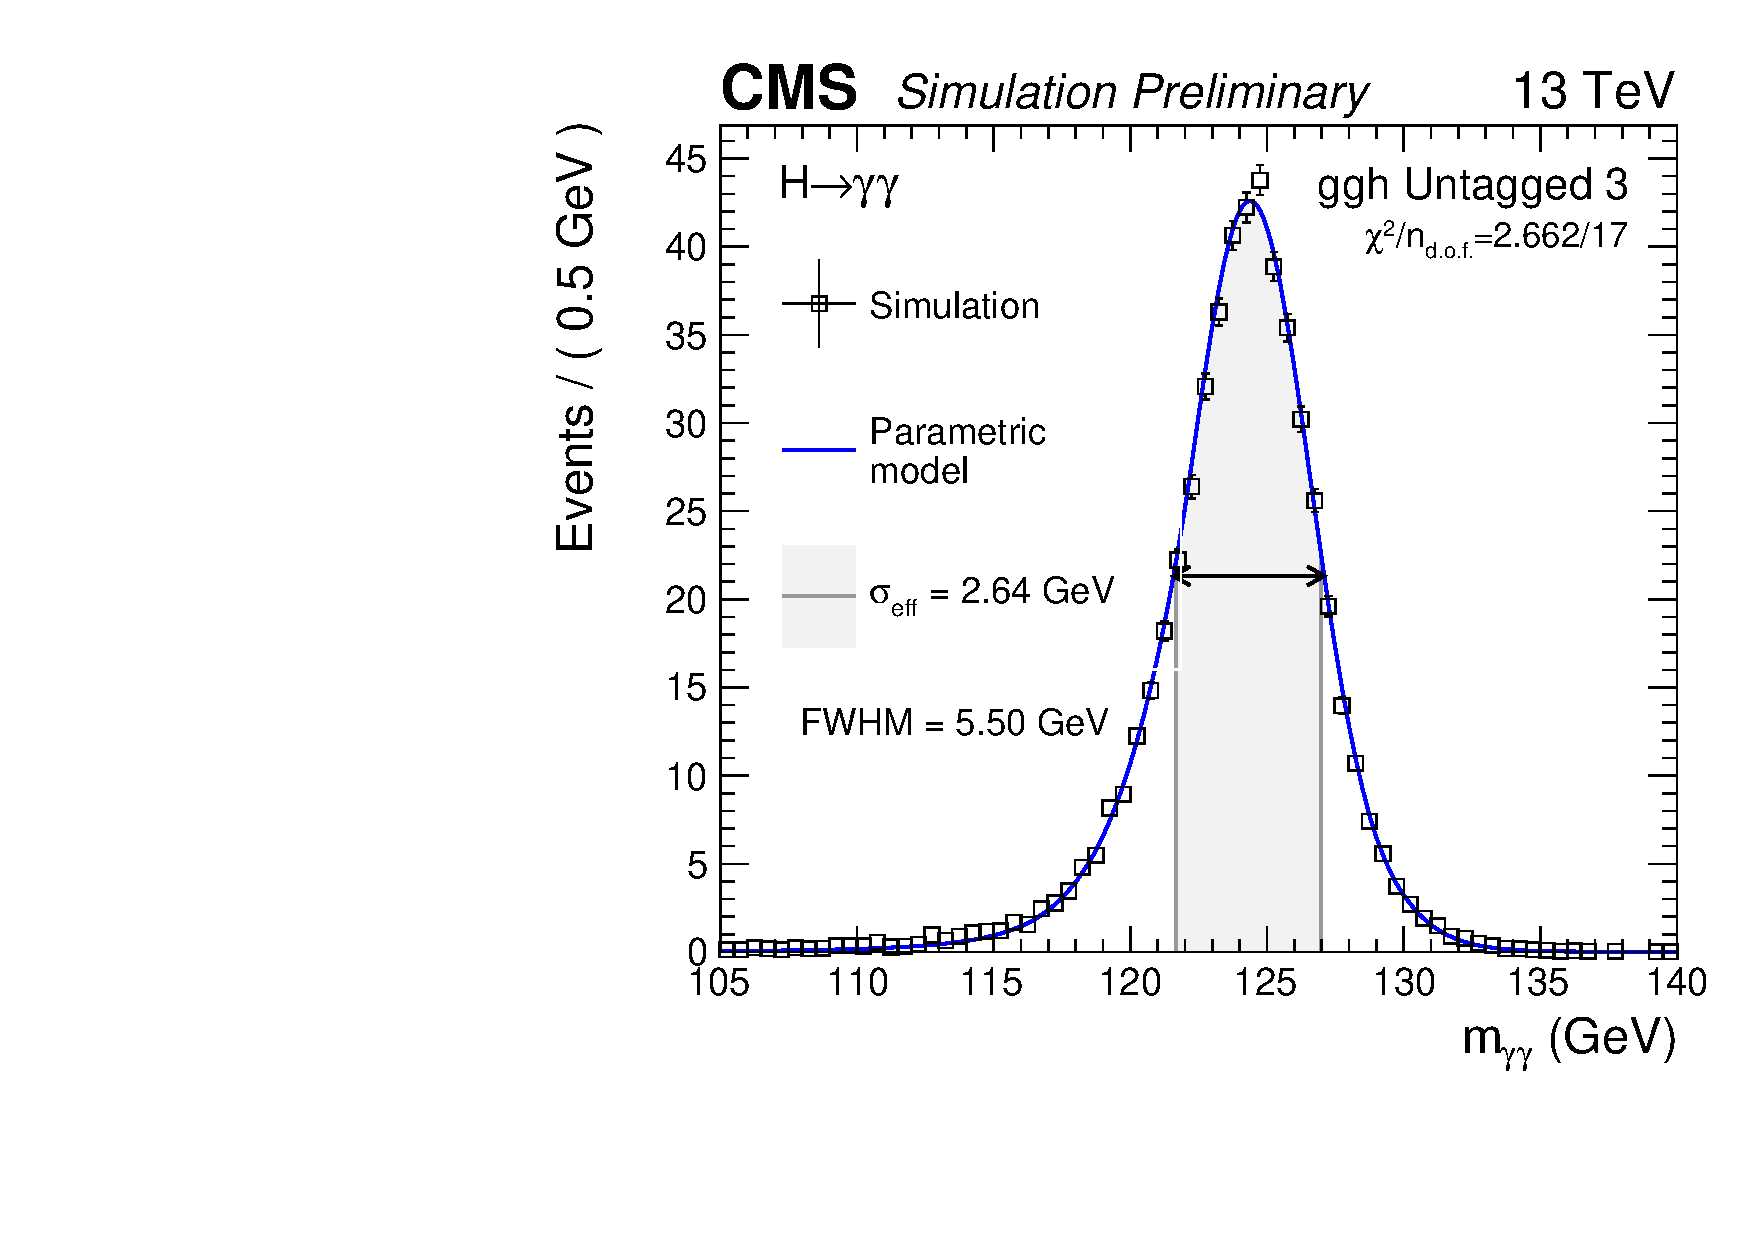
\includegraphics[width=0.3\textwidth]{modellingFigures/DCBpG/ggh_UntaggedTag_3.pdf} 
}}\\
  \subfloat[Functional form: Sum of Gaussians]{\shortstack{
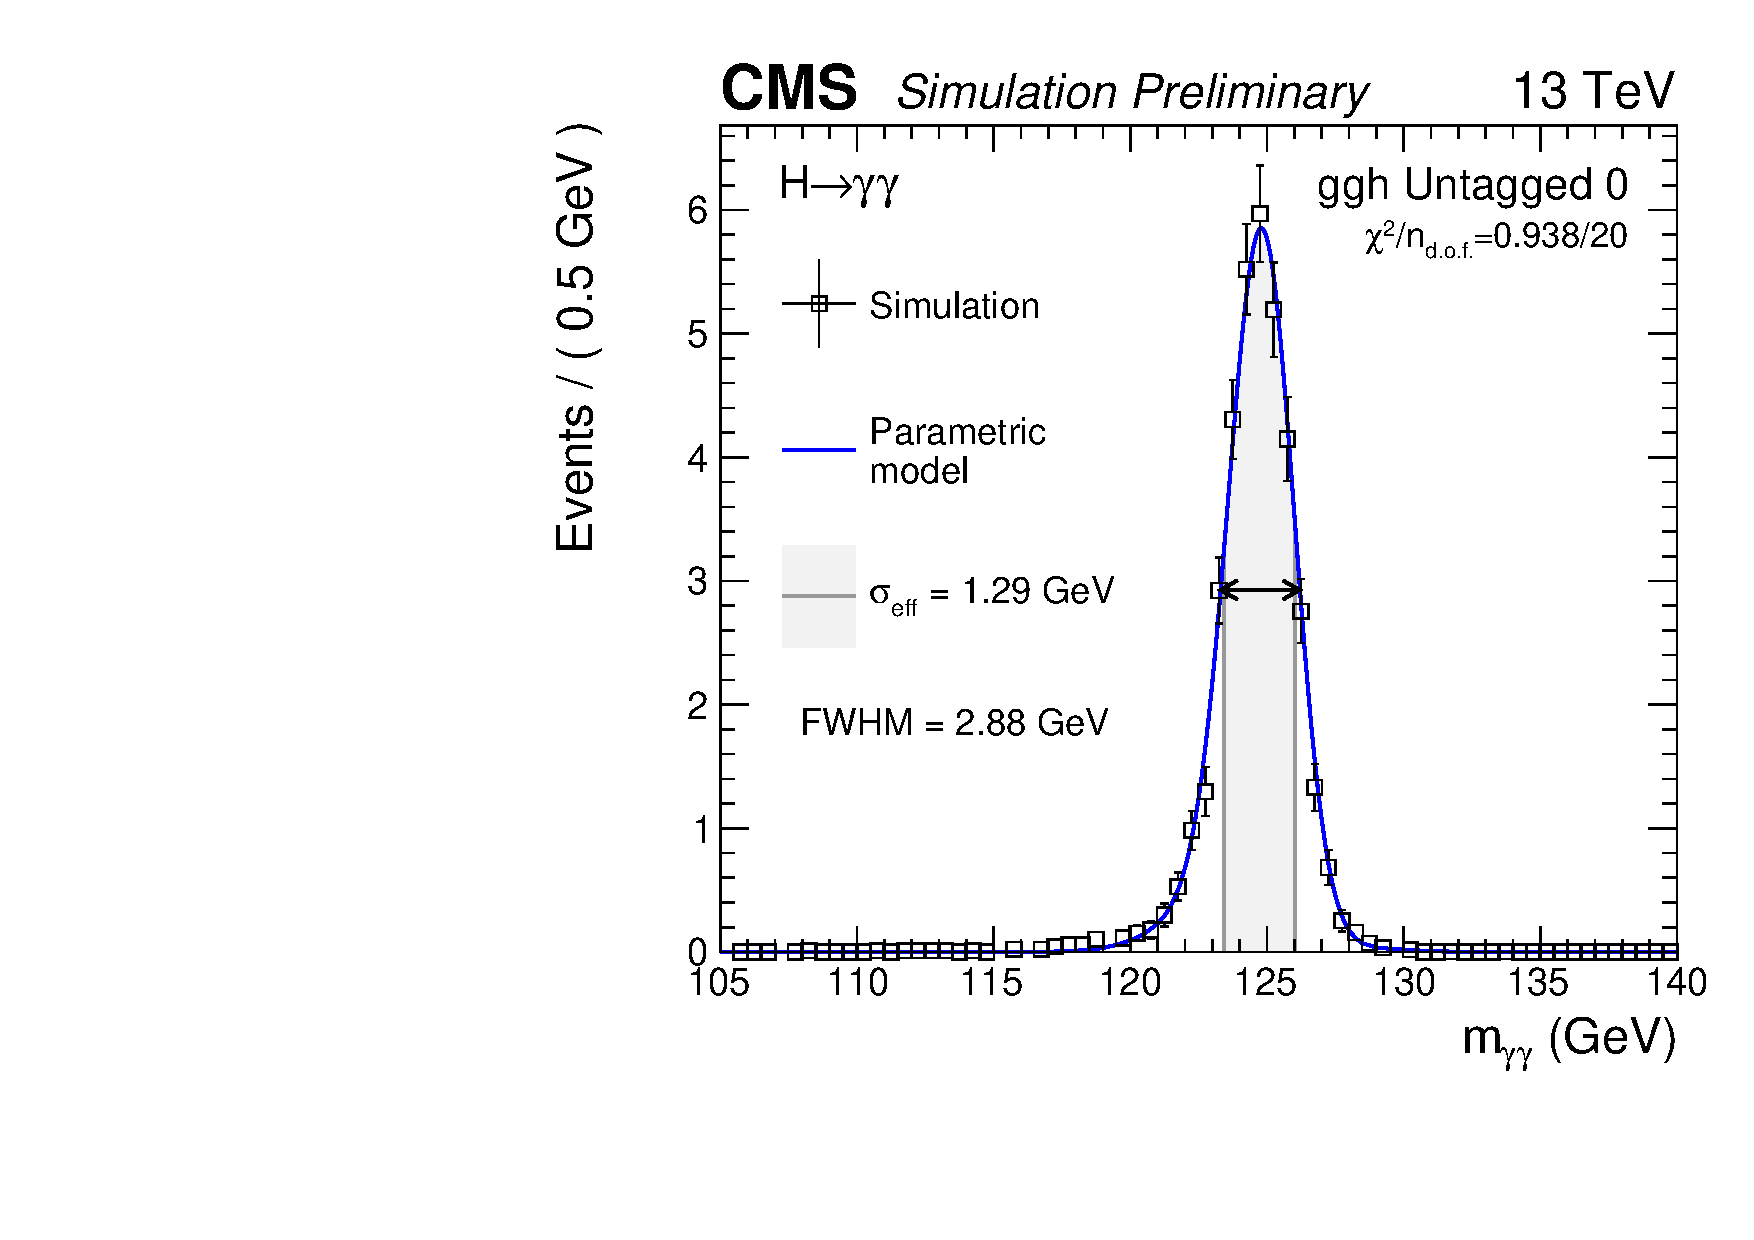
\includegraphics[width=0.3\textwidth]{modellingFigures/nGaus/ggh_UntaggedTag_0.pdf} 
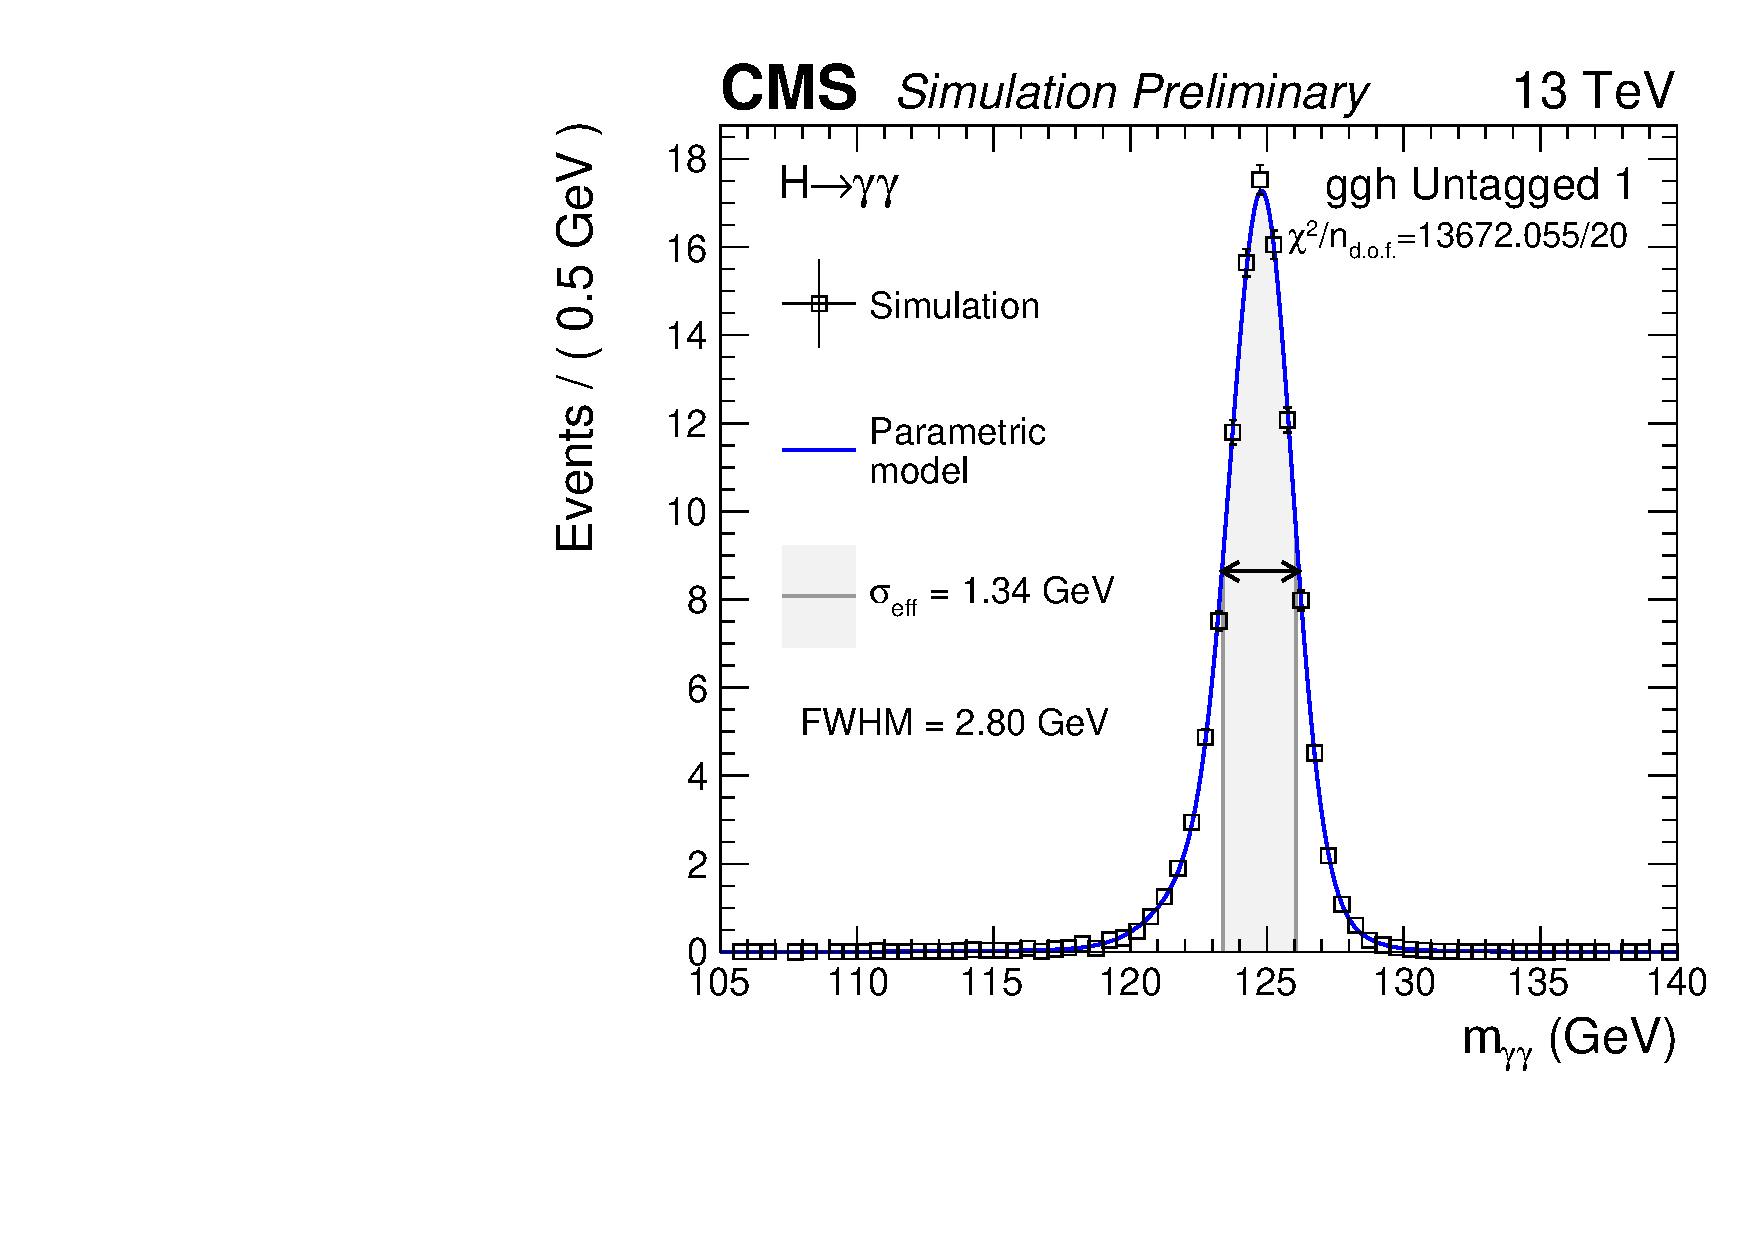
\includegraphics[width=0.3\textwidth]{modellingFigures/nGaus/ggh_UntaggedTag_1.pdf}\\  
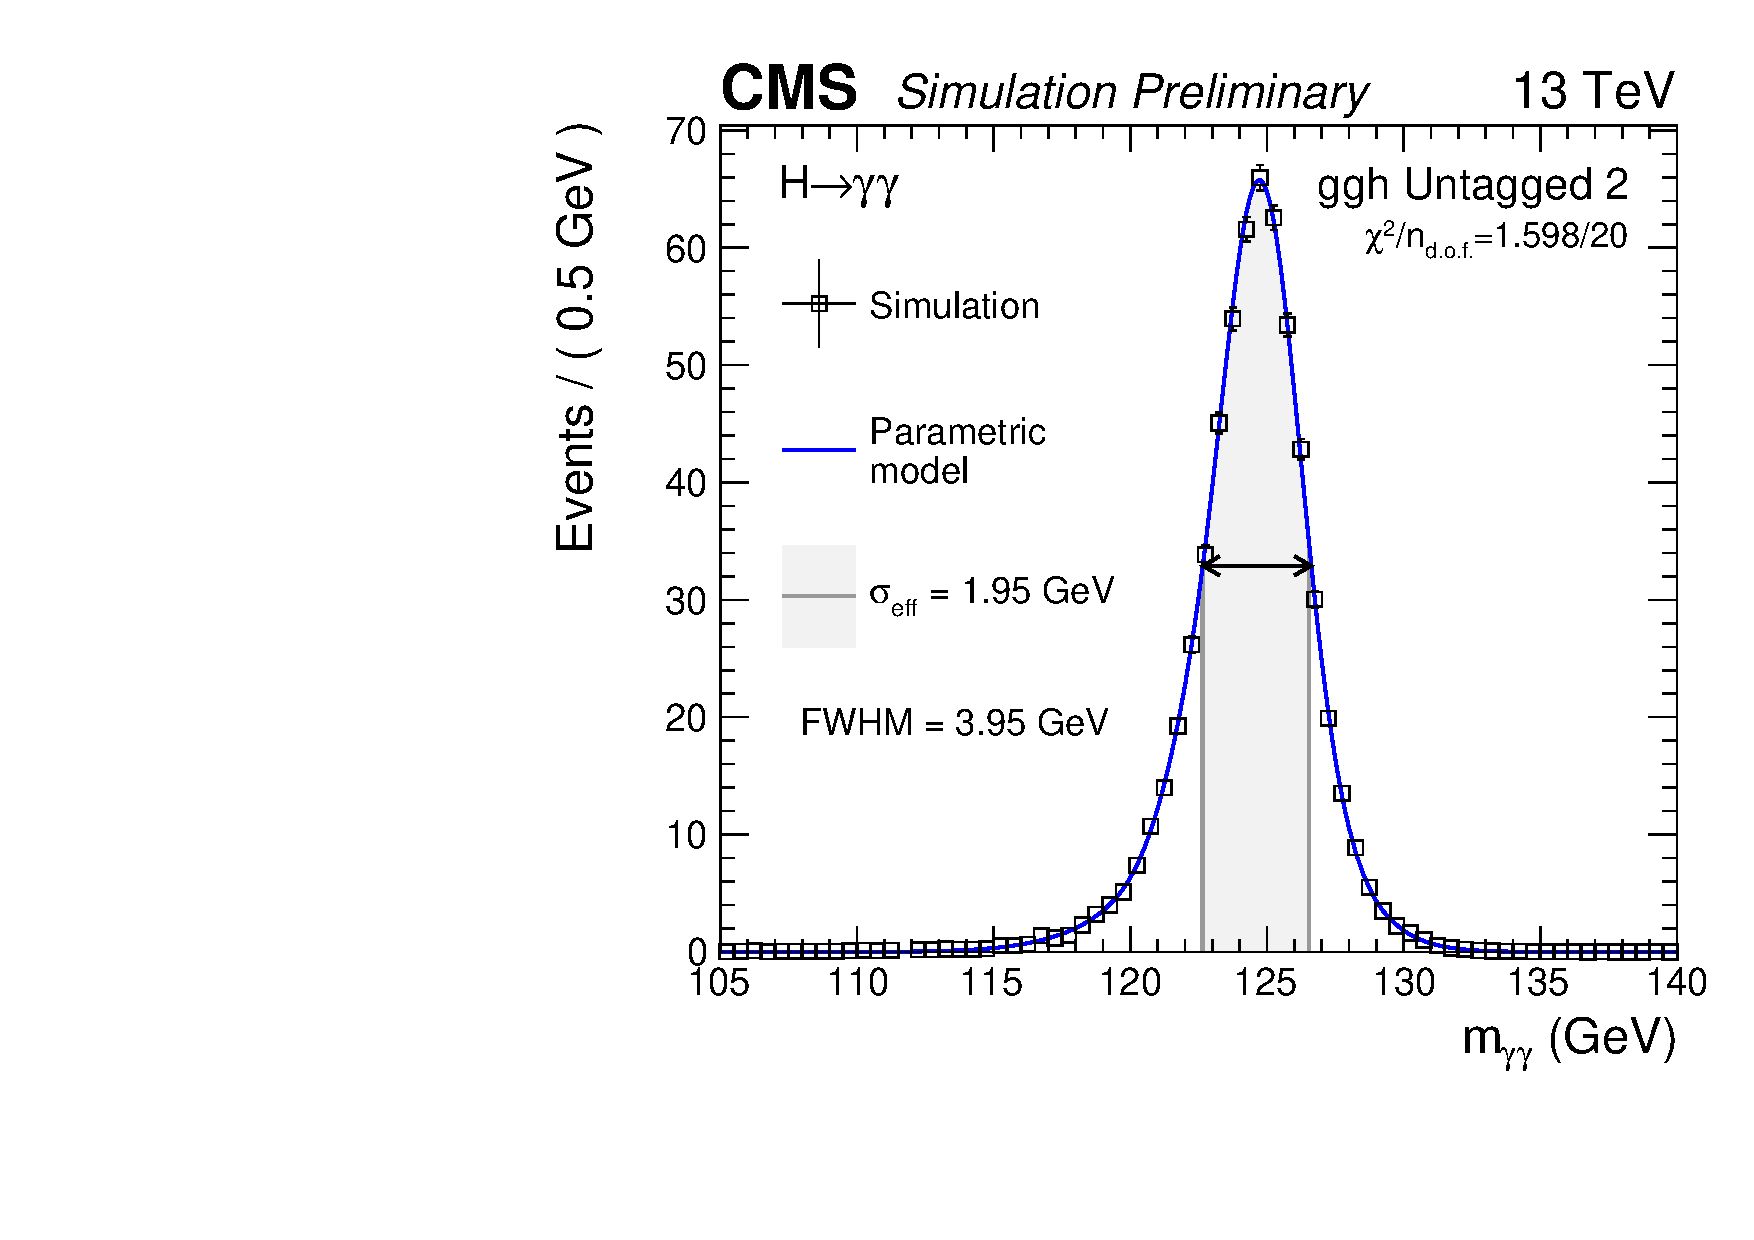
\includegraphics[width=0.3\textwidth]{modellingFigures/nGaus/ggh_UntaggedTag_2.pdf} 
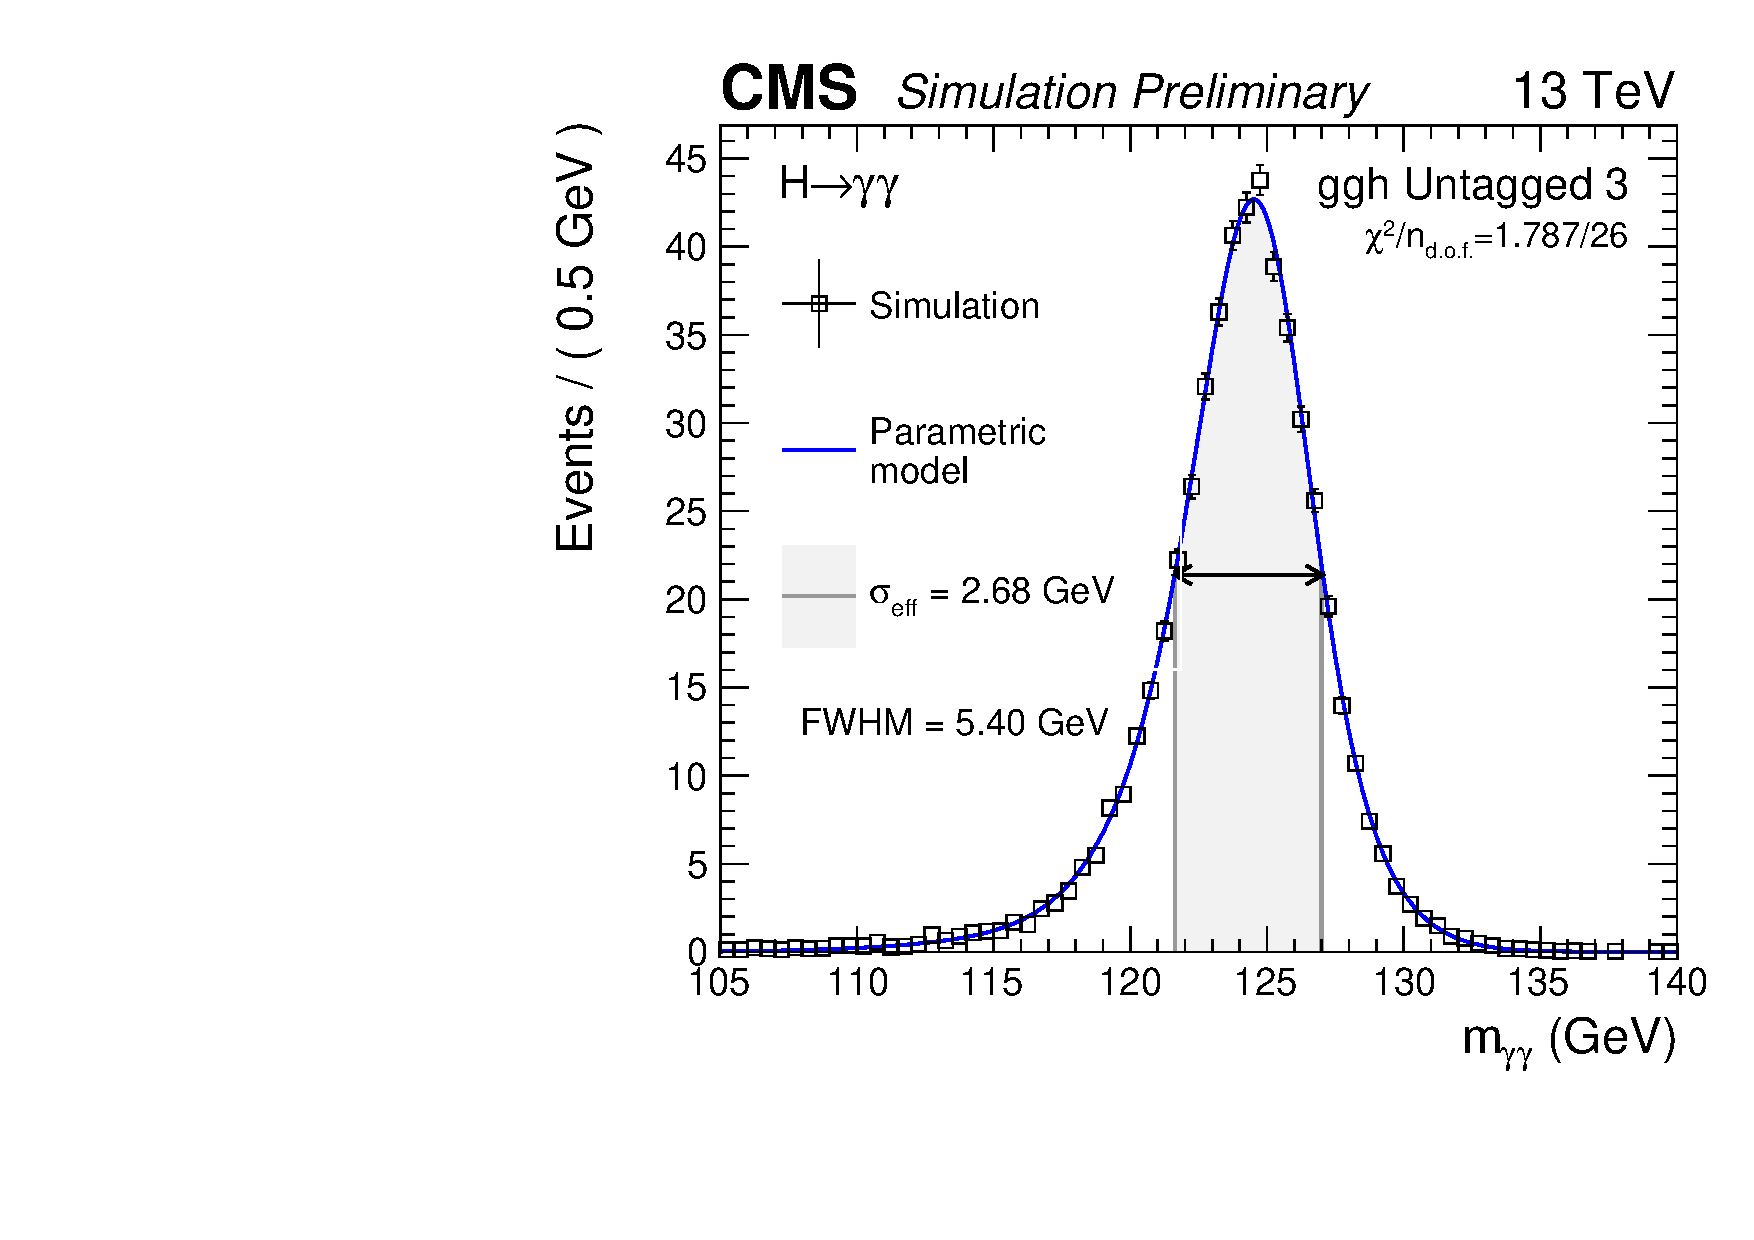
\includegraphics[width=0.3\textwidth]{modellingFigures/nGaus/ggh_UntaggedTag_3.pdf} 
}}
\caption{The shape of the simulated \mgg distribution (\mH=125\GeV) for the \ggH process for the inclusive categories when parametrised with (a) \DCBpG and (b) sum of Gaussians, where the RV and WV contributions have been summed according to their relative yield. The plots show the agreement between the simulation and the parametrisation expressed as the $\chi^2$, alongside the total number of degrees of freedom in the parametrisation.}

\label{fig:model:functionalform}
\end{figure}

%A number of checks were performed to validate the use of the \DCBpG shape
%insert tests of different functional forms / appendix ?
%tests on DCB response to signal systematics / appendix ?
%bias studies involving DCB shape / appendix ?
%If the number of events in the sample after splitting into provess, category adn \RV/WV case is too low, it can be extremnely difficult to meaningully fit the \DCB1G shape. In this case, a replacement shape from a related high-statistics category is used to model this tag/process.

\subsection{Dependence of model on \mH}

Since the mass of the Higgs boson is not exactly known, the parametrisations from simulated signal samples assuming different \mH values are combined to form a single parametric model. There are two methods to perform this combination. 
The first option is to perform the fitting procedure described above for each \mH case. The individual parameters of the functional form can then be linearly interpolated from one \mH case to the next to produce the parametric model. This is the approach taken in~\cite{LegacyHgg,CMS-PAS-HIG-15-005,CMS-PAS-HIG-16-020}.

The second option, which is used in this analysis, instead performs a simultaneous fit of all the different \mH samples, where the individual parameters of the functional form are themselves polynomials of \mH. %The fitting procedure can then occur for all mass cases at once, where 
The floating parameters in the fit are then the coefficients of these polynomials. % (functions of \mH) representing each parameter of the functional form (a function of \mgg). 
The advantage of this method, which is referred to as \SSF, is a reduction in the total number of parameters used to determine the full model. %Indeed, in the linear interpolation method, the total number of floating parameters is increased for sample with a new \mH, since it is parameterised separately from the others. In the \SSF method the additional degrees of freedom come only from the chosen order of the polynomial describing the parameters in the main functional form). 
Furthermore, the \SSF method guarantees a sensible parametric model, whereas the linear interpolation method can lead to discontinuous or unphysical models since the individual \mH cases are parametrised separately and therefore are not guaranteed to be consistent. 

The \SSF method is applied separately for each process, category and \RV or \WV case, using seven different \mH cases: 120, 123, 124,125, 126, 127 and 130\GeV. The description of the parameters of the \DCBpG function uses polynomials of order 1. Polynomials of order 0, 1 and 2 were all tested, but it was found that there was no substantial improvement in the agreement when using an order greater than 1. This was determined to be because the floating parameters were not sufficiently constrained by the simulated \mgg distributions to bring any meaningful improvement.

The signal models for the \RV and \WV contributions are combined according to their relative event content. The fraction of events where the selected vertex was within $1\cm$ in the $z$-direction from the true vertex is evaluated for each \mH sample, and then parametrised as a first order polynomial to get a smooth dependence on \mH. 

The dependence of the full parametric signal model on \mH for the \ggH process in each of the analysis categories is shown in \Fig~\ref{fig:model:sig_interpolation}. 

\begin{figure}[ht!]
\centering
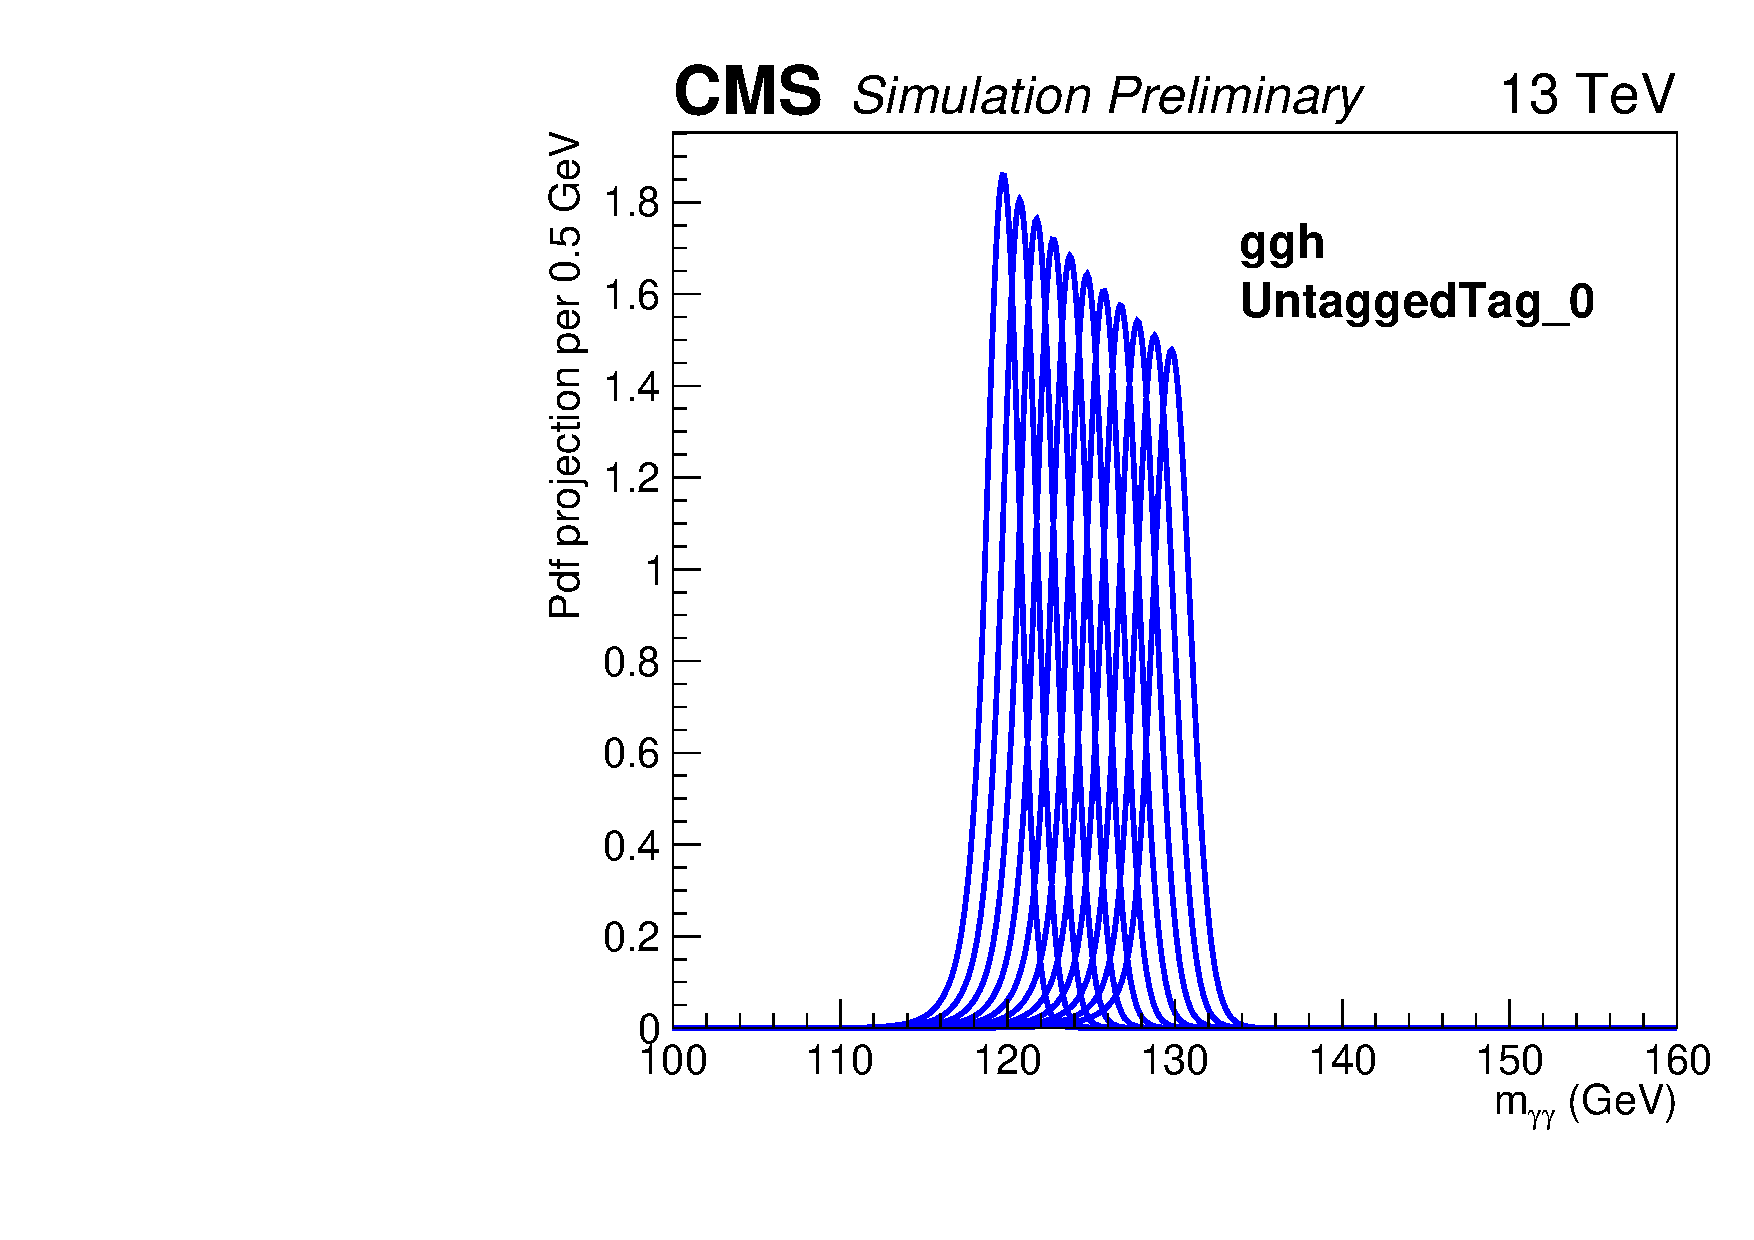
\includegraphics[width=0.3\textwidth]{modellingFigures/DCBpG/ggh_UntaggedTag_0_fmc_interp.pdf} 
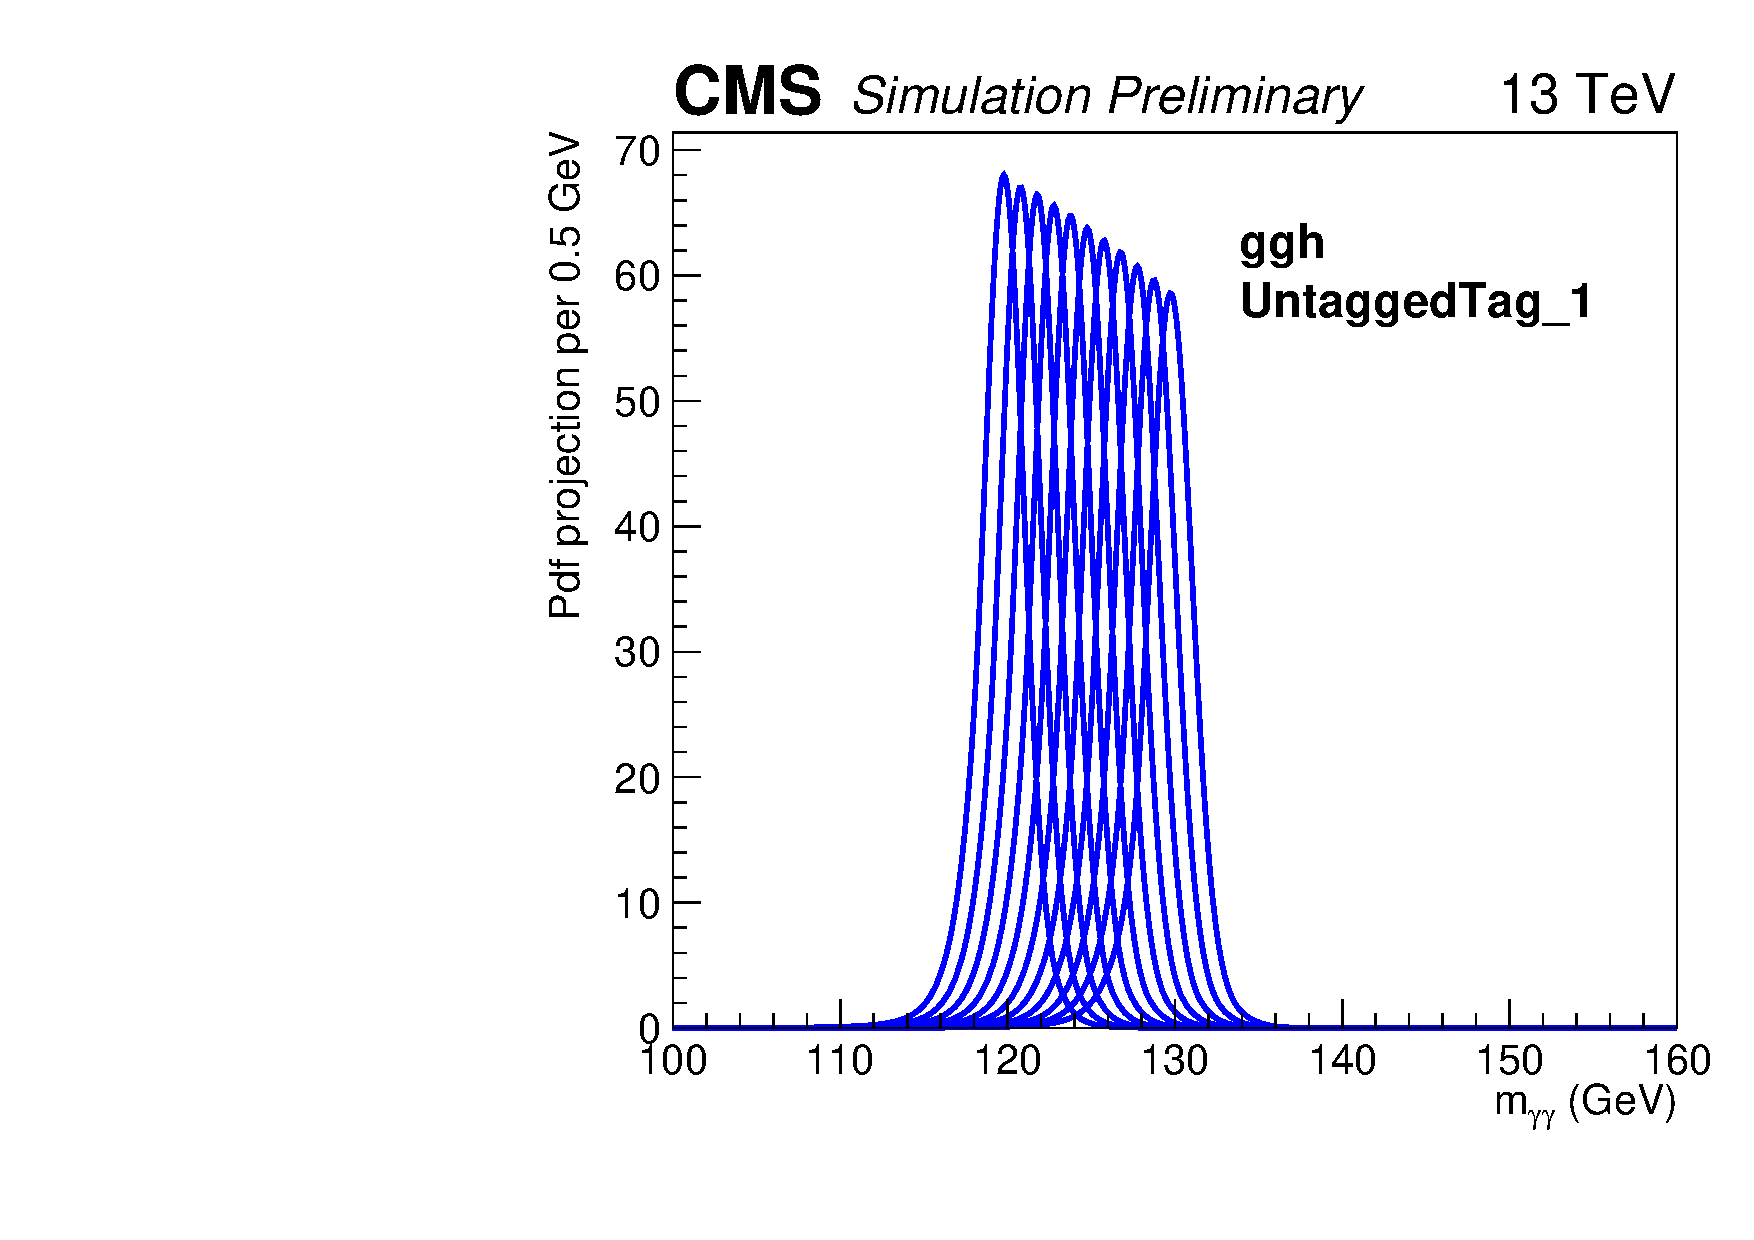
\includegraphics[width=0.3\textwidth]{modellingFigures/DCBpG/ggh_UntaggedTag_1_fmc_interp.pdf} \\ 
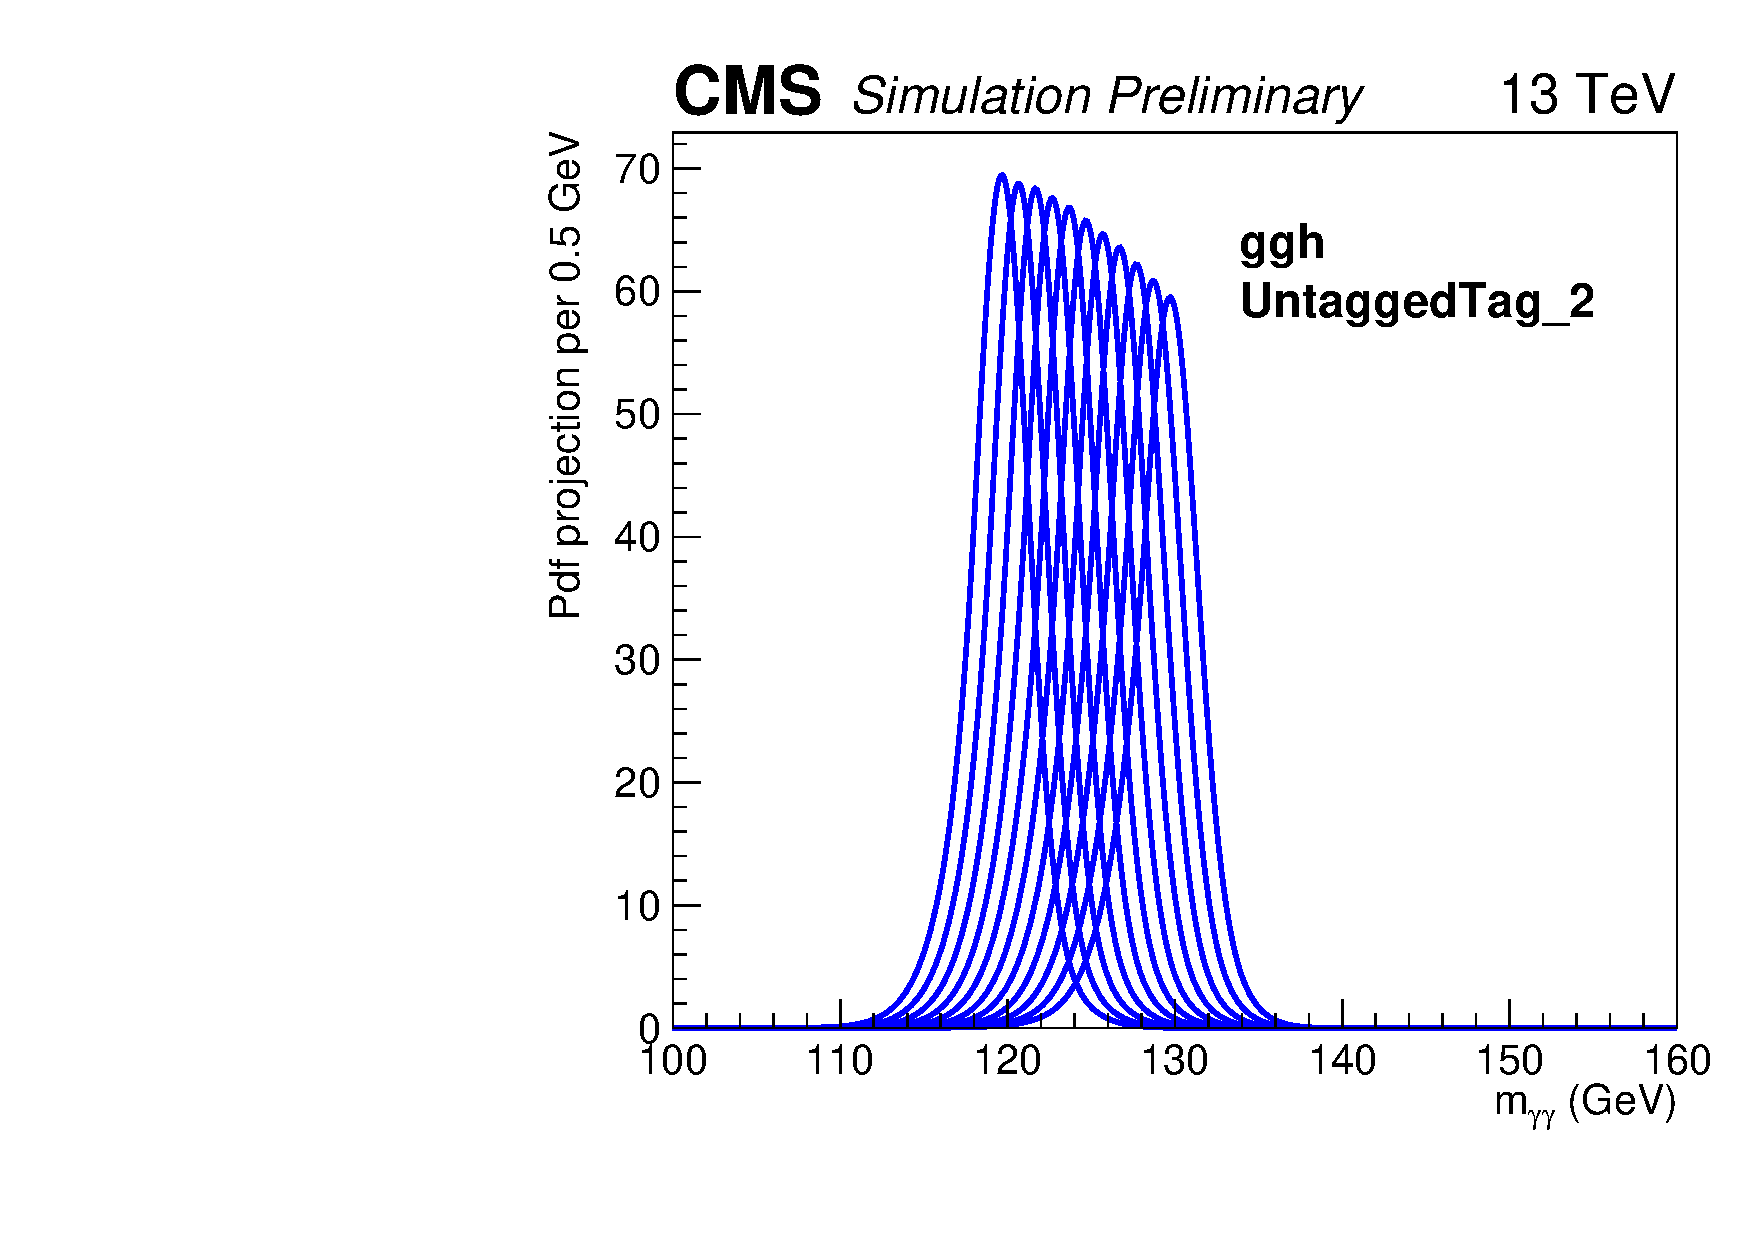
\includegraphics[width=0.3\textwidth]{modellingFigures/DCBpG/ggh_UntaggedTag_2_fmc_interp.pdf} 
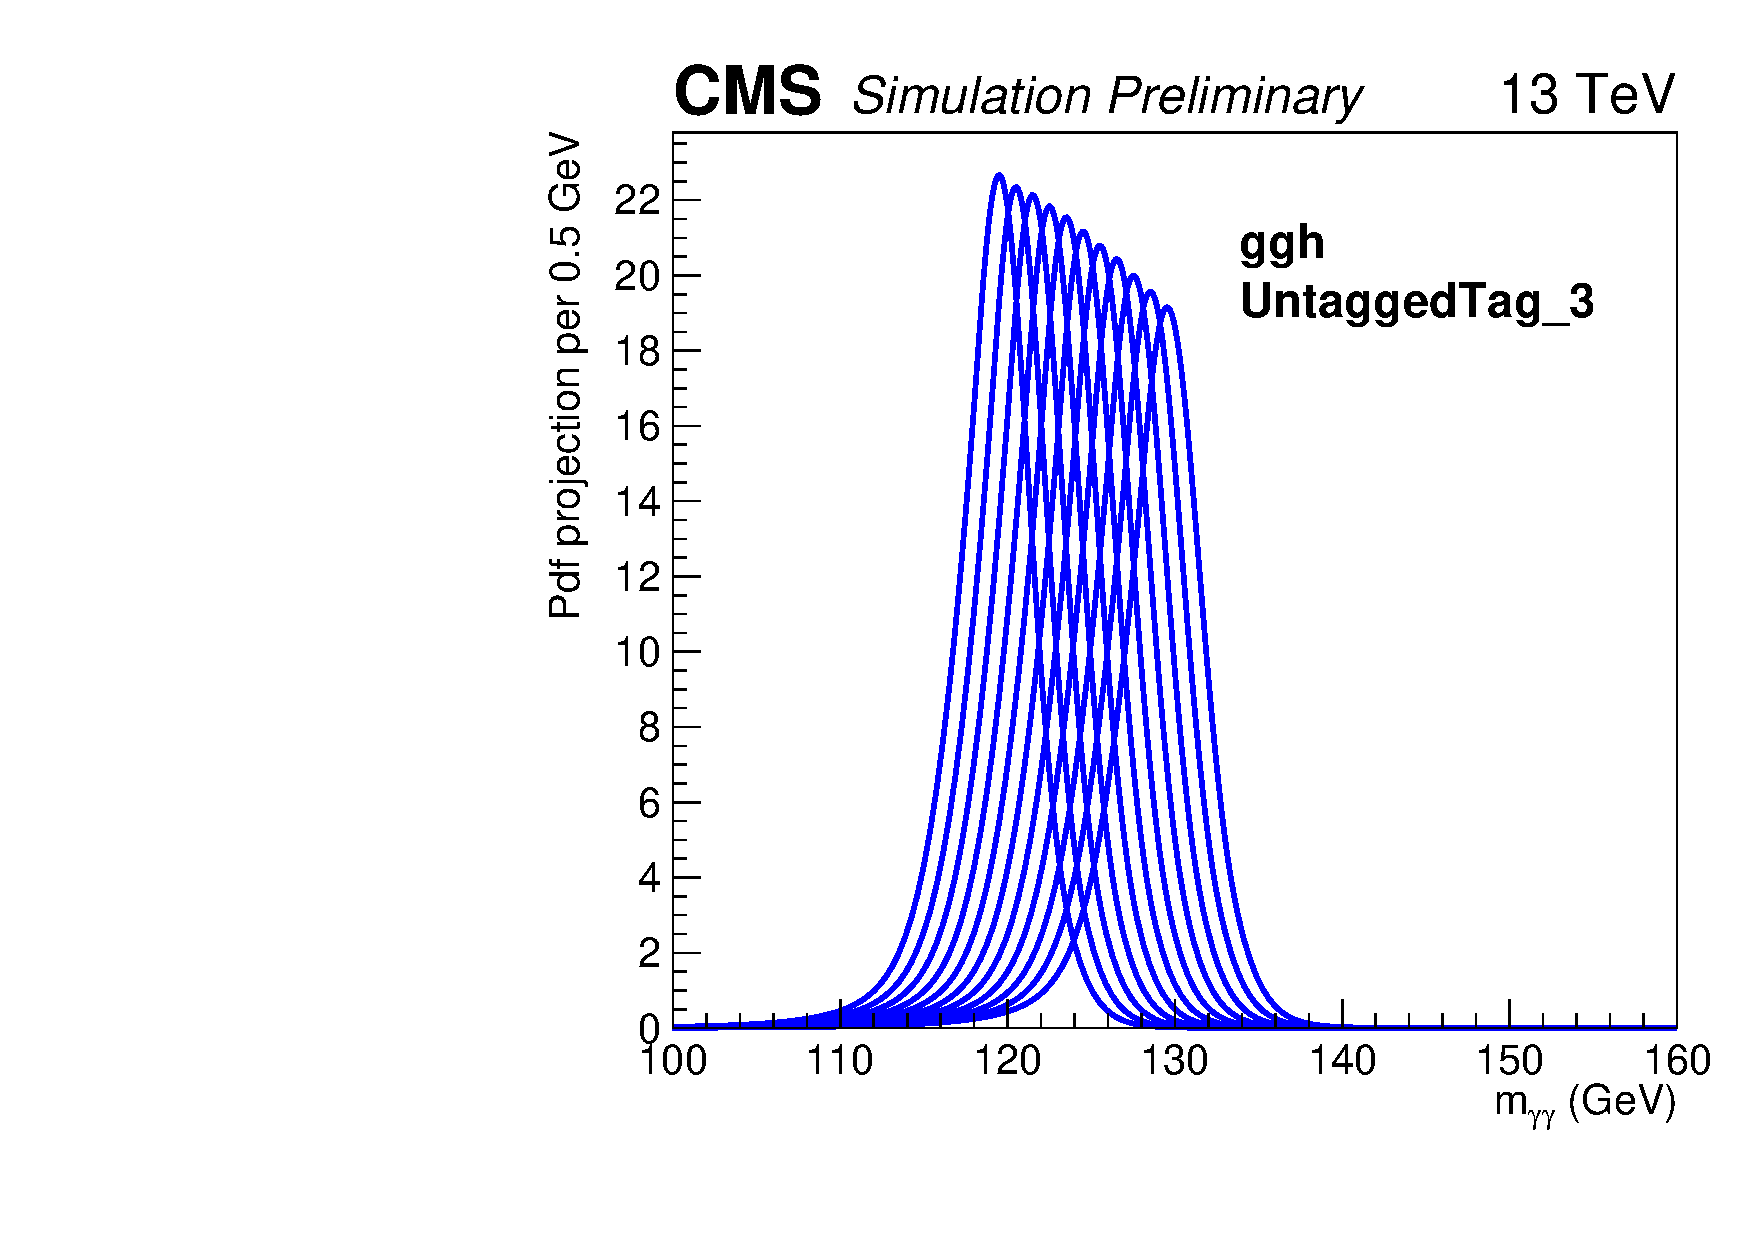
\includegraphics[width=0.3\textwidth]{modellingFigures/DCBpG/ggh_UntaggedTag_3_fmc_interp.pdf} \\
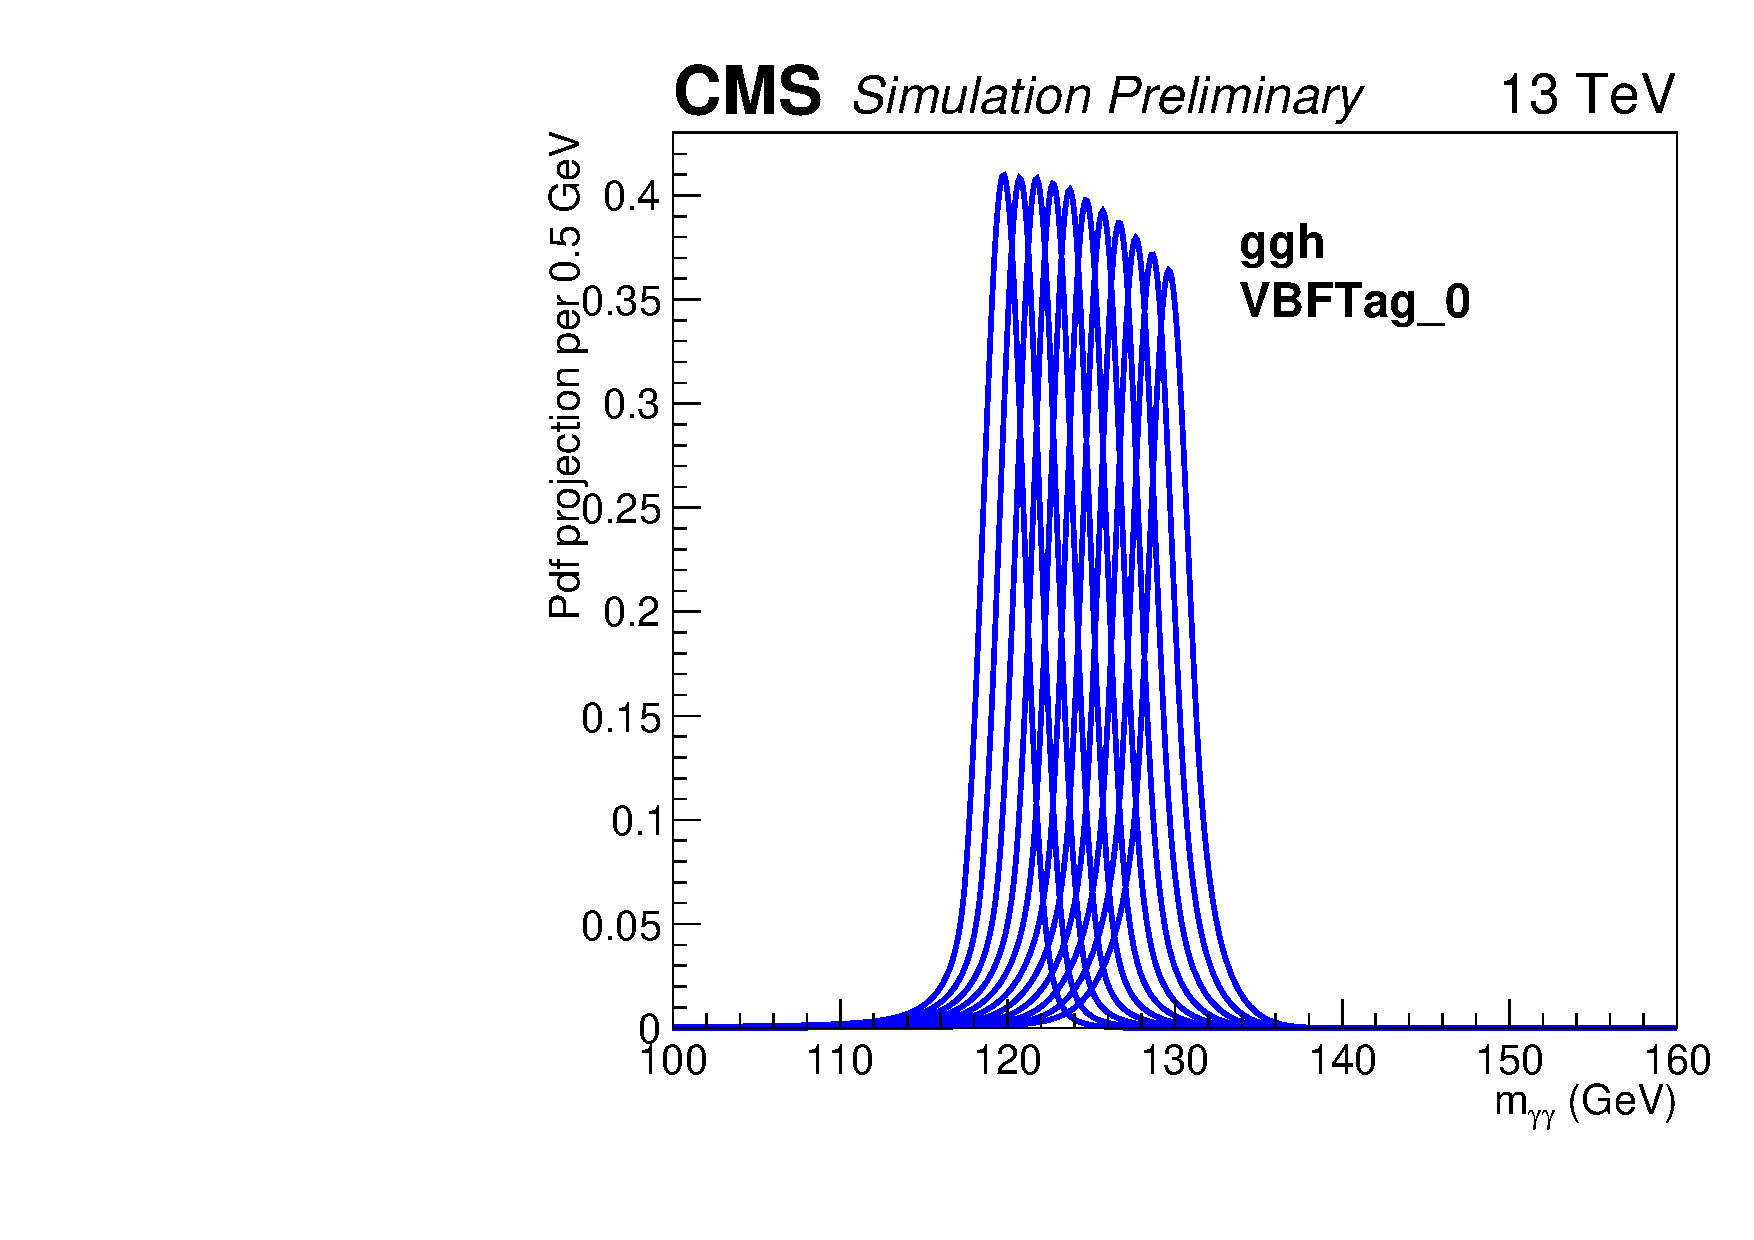
\includegraphics[width=0.3\textwidth]{modellingFigures/DCBpG/ggh_VBFTag_0_fmc_interp.pdf} 
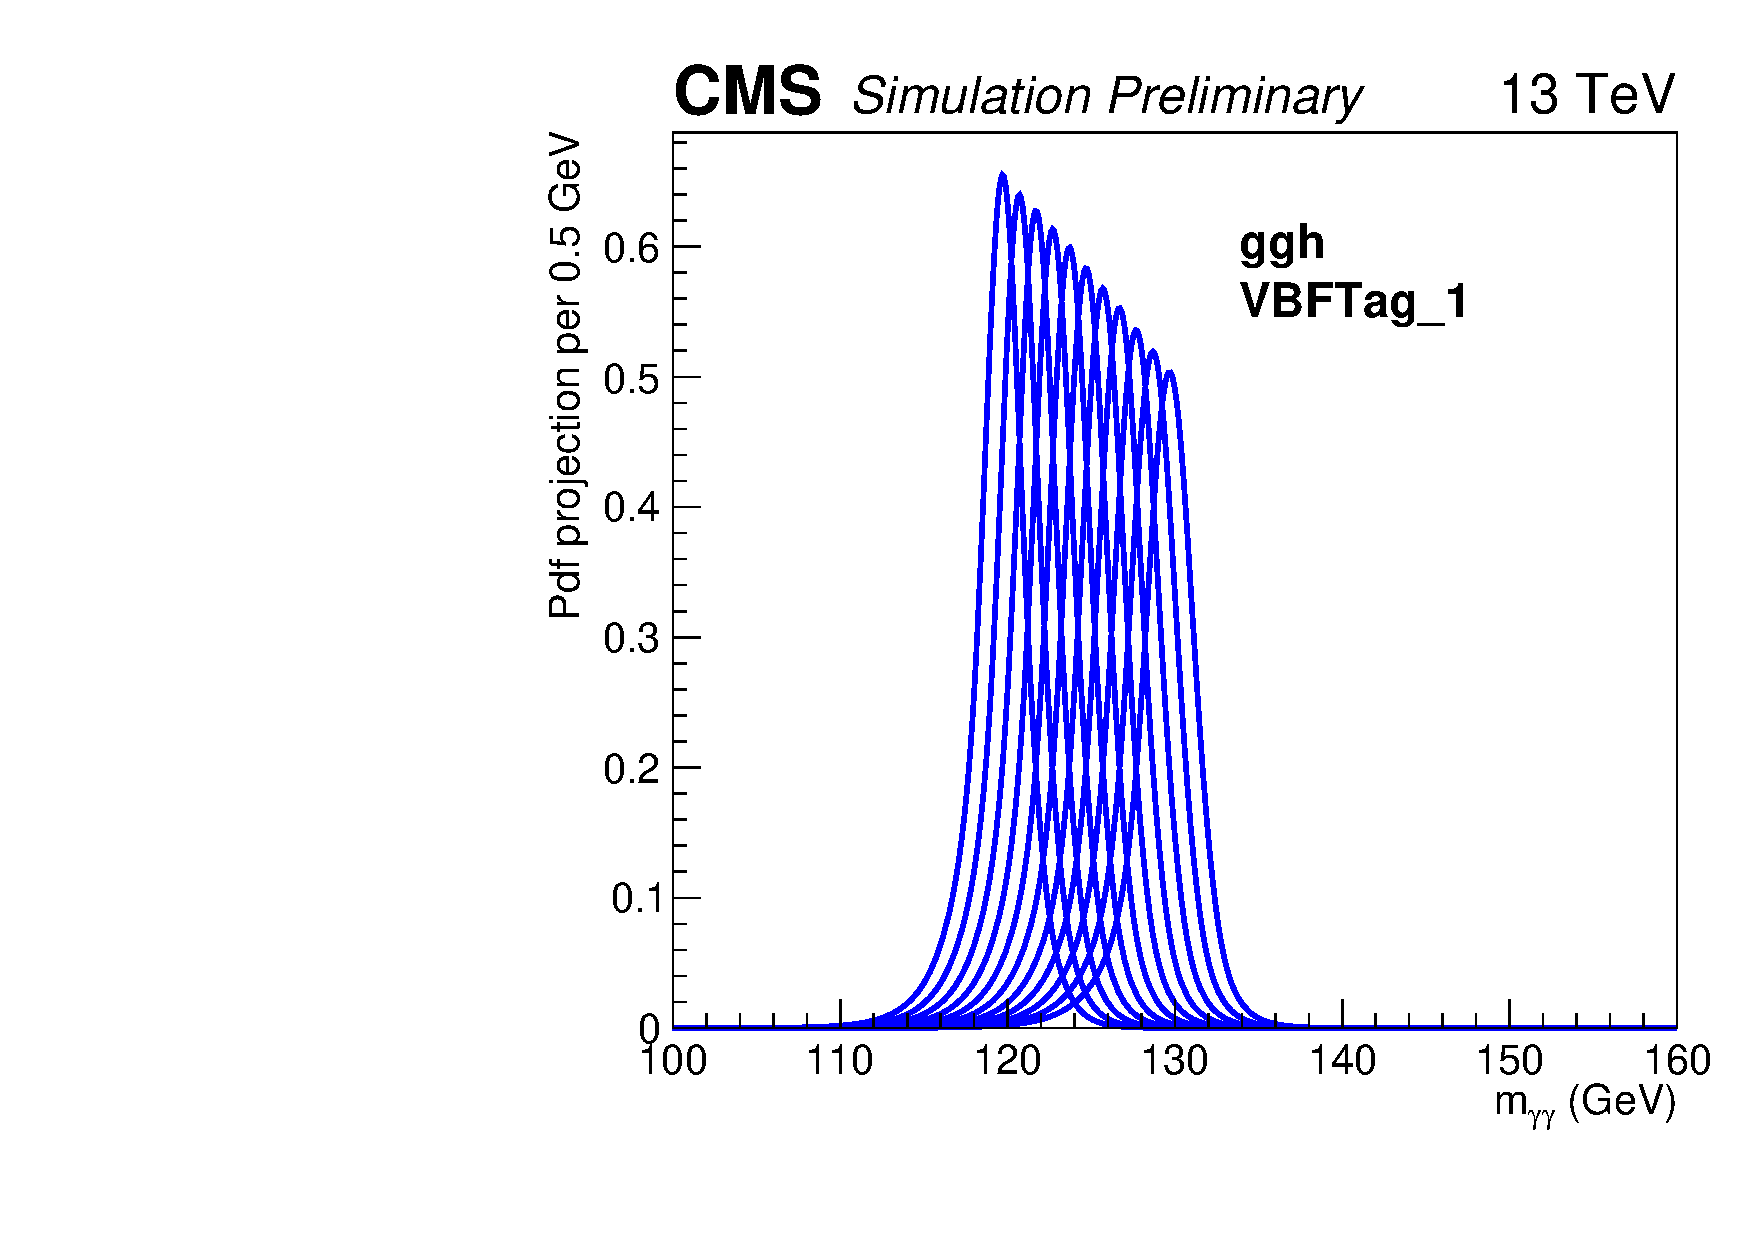
\includegraphics[width=0.3\textwidth]{modellingFigures/DCBpG/ggh_VBFTag_1_fmc_interp.pdf} \\
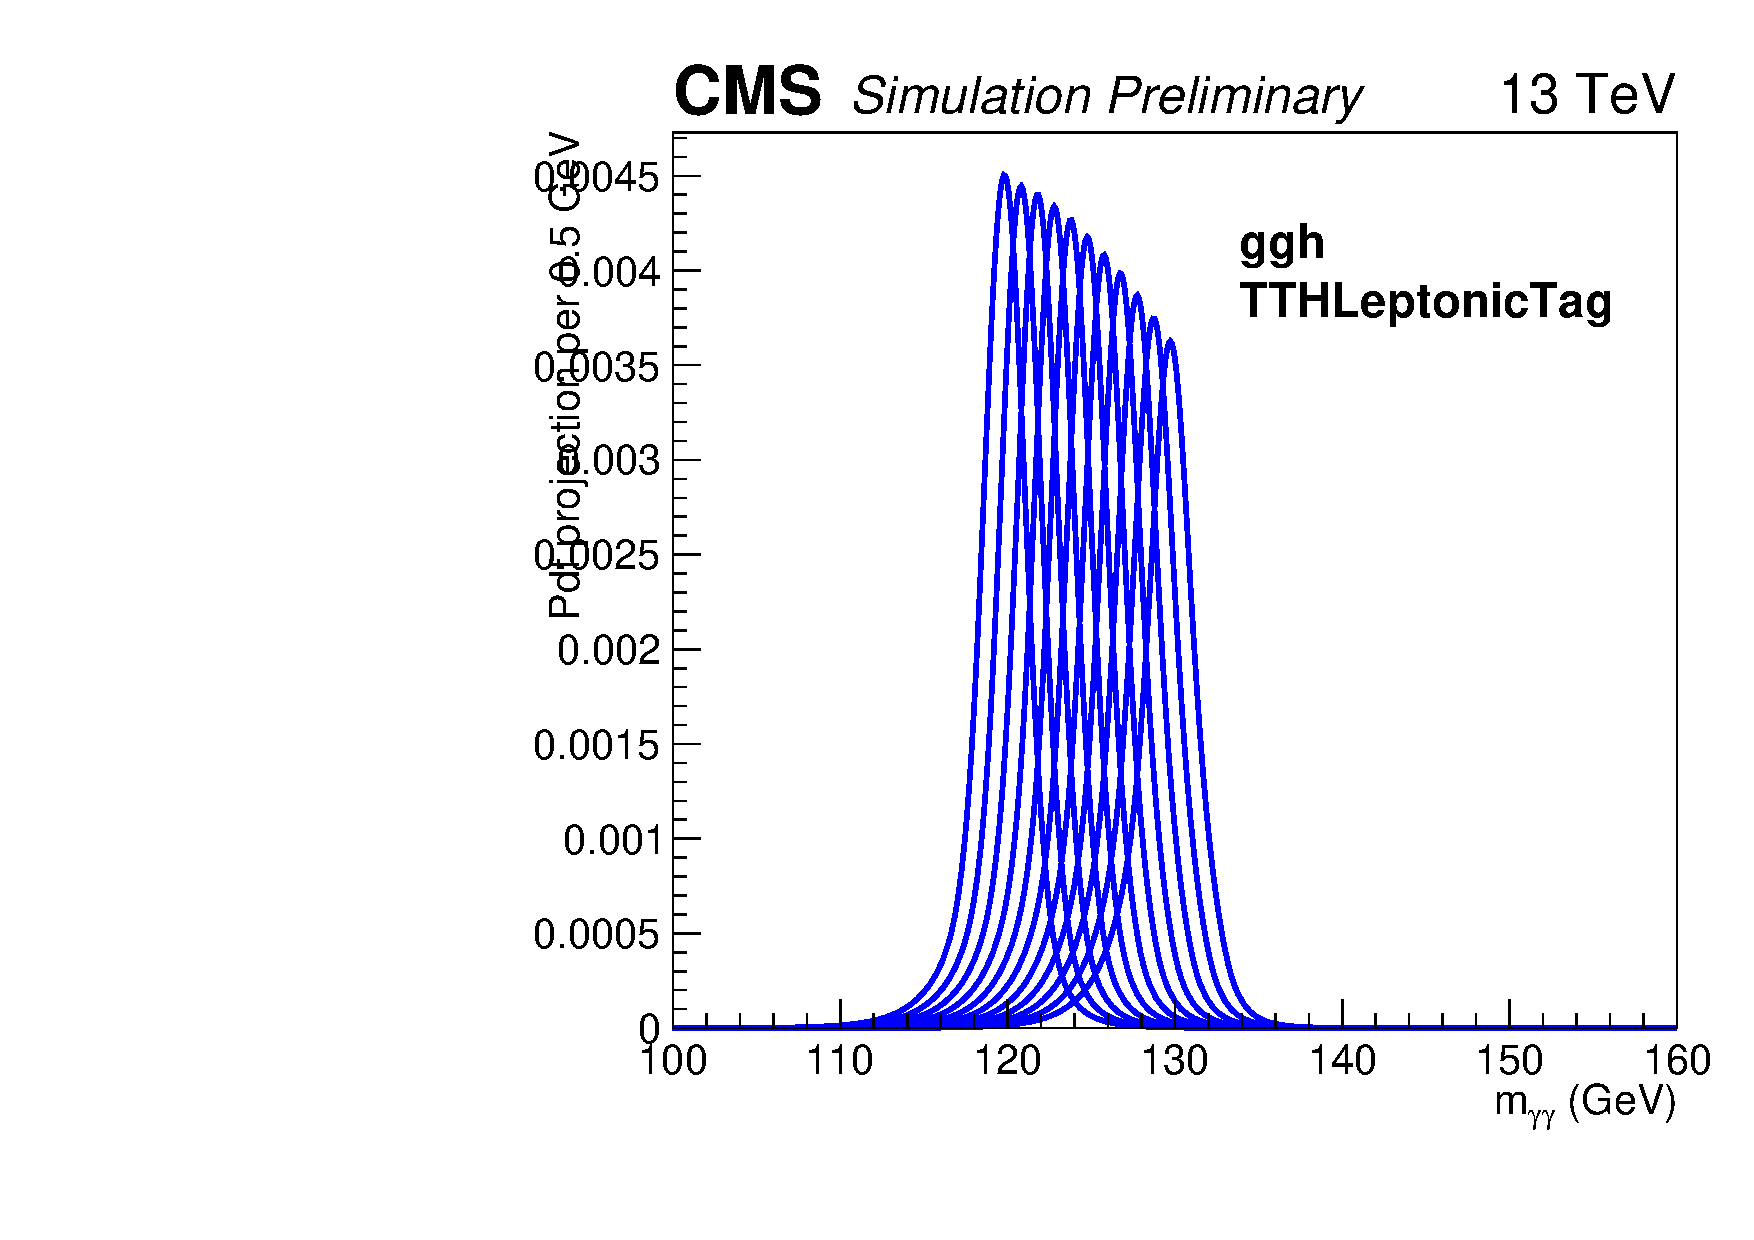
\includegraphics[width=0.3\textwidth]{modellingFigures/DCBpG/ggh_TTHLeptonicTag_fmc_interp.pdf} 
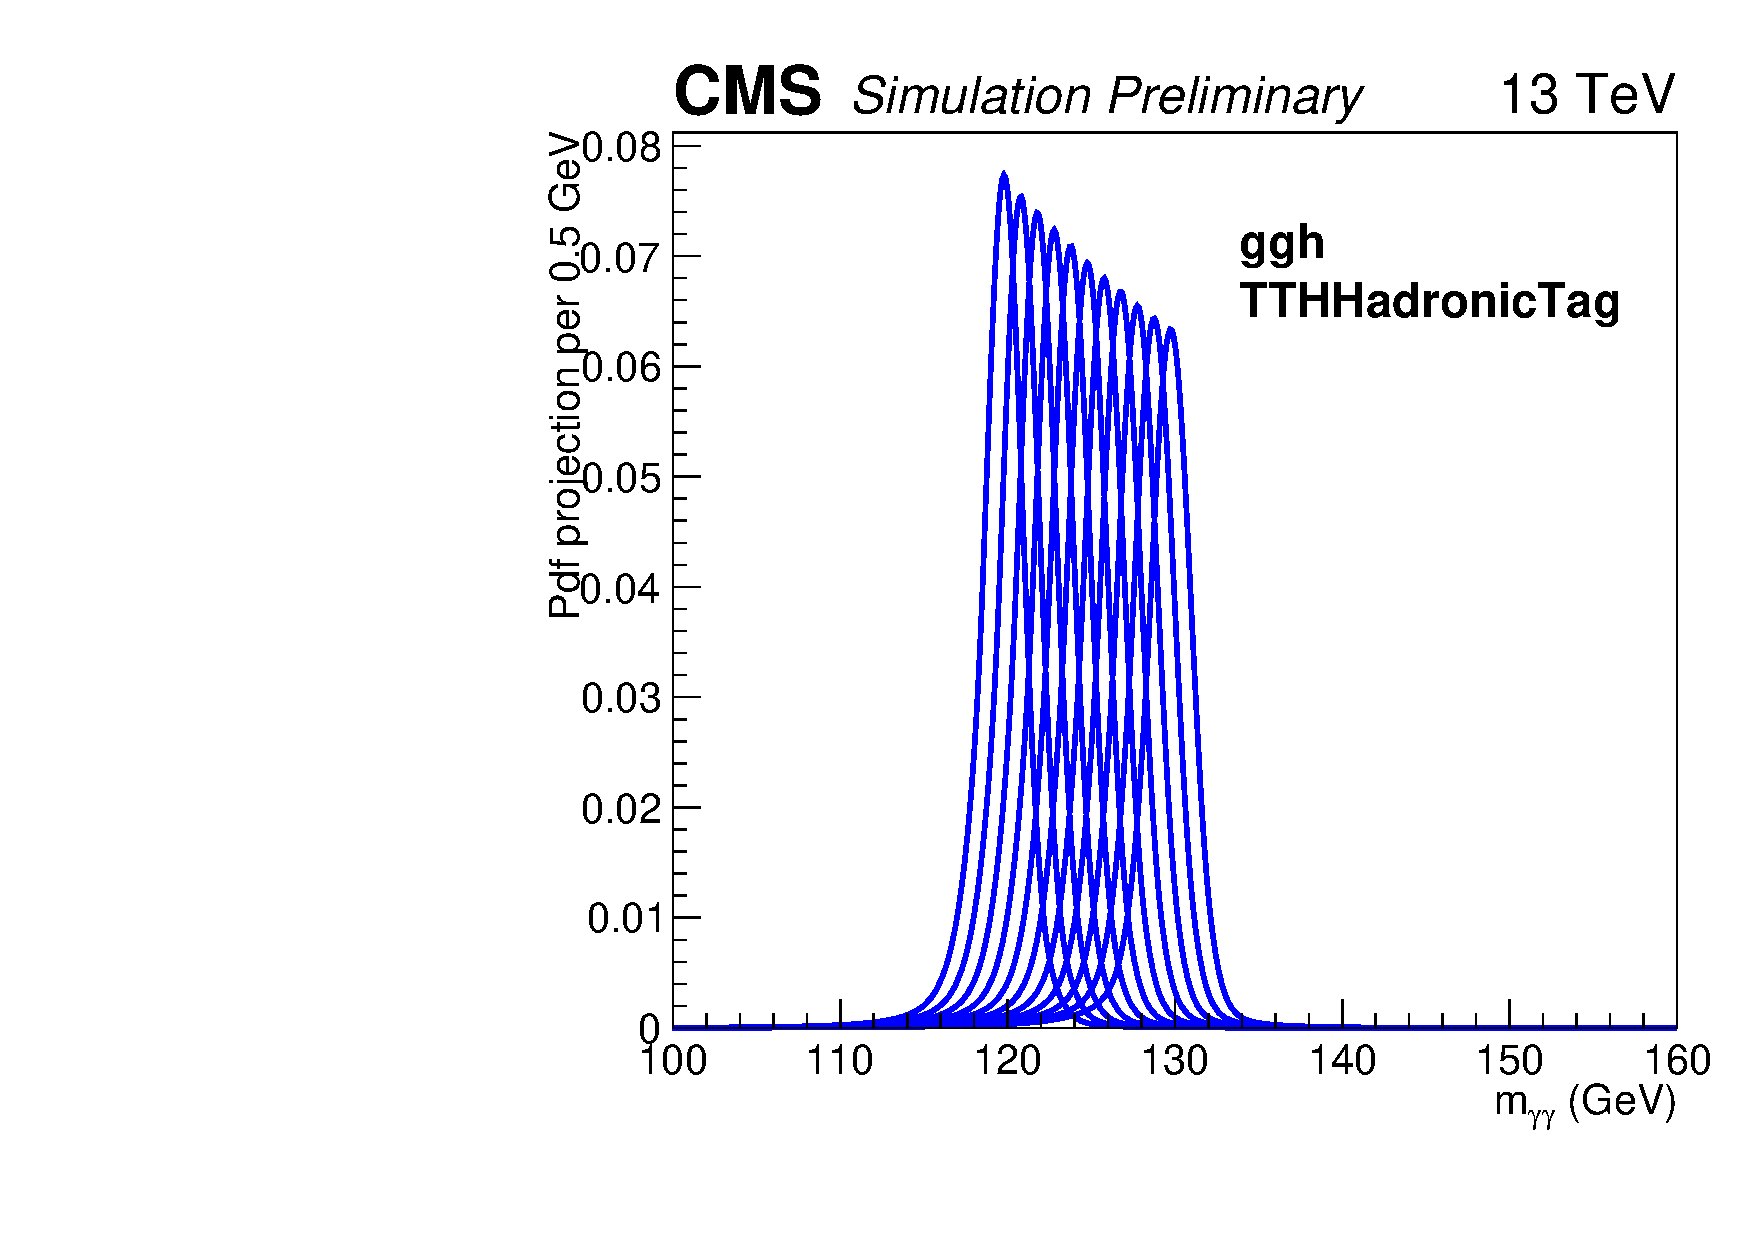
\includegraphics[width=0.3\textwidth]{modellingFigures/DCBpG/ggh_TTHHadronicTag_fmc_interp.pdf} 
\caption{The \mH-dependence of the signal models for the ggH process for each of the analysis categories is shown. Each curve shows the signal model for a given value of \mH. The contributions from the RV and WV components of each model were summed together according to their relative size, linearly interpolated between the samples for different \mH.}

\label{fig:model:sig_interpolation}
\end{figure}

\subsection{Normalisation of signal models}

The signal models are normalised to match the number of event predicted by the \SM after detector acceptance ($A$) and selection efficiency ($\epsilon$) are taken into account. The expected number of events in each sample (ignoring $A$ and $\epsilon$) is first computed as the product of the relevant process \crosssection, the \Hgg branching fraction and the integrated luminosity of the data sample. The \crosssection\s and branching fraction, as well as their dependence on \mH, are obtained from the \LHCHXSWG recommendation~\cite{LHCHXSWGYR4}. After the simulated samples have been reconstructed and the events selected and categorised, the number of remaining events is related to the expected number by \effxacc, which is parametrised in \mH using a polynomial fit. The final normalisation of the signal models for an arbitrary value of \mH can then be obtained from the parametrised \effxacc multiplied by the total number of events exected by the \SM. \Fig~\ref{fig:model:sig_effxacc} shows the overall \effxacc for all categories combined as a function of \mH.

\begin{figure}[ht!]
\centering
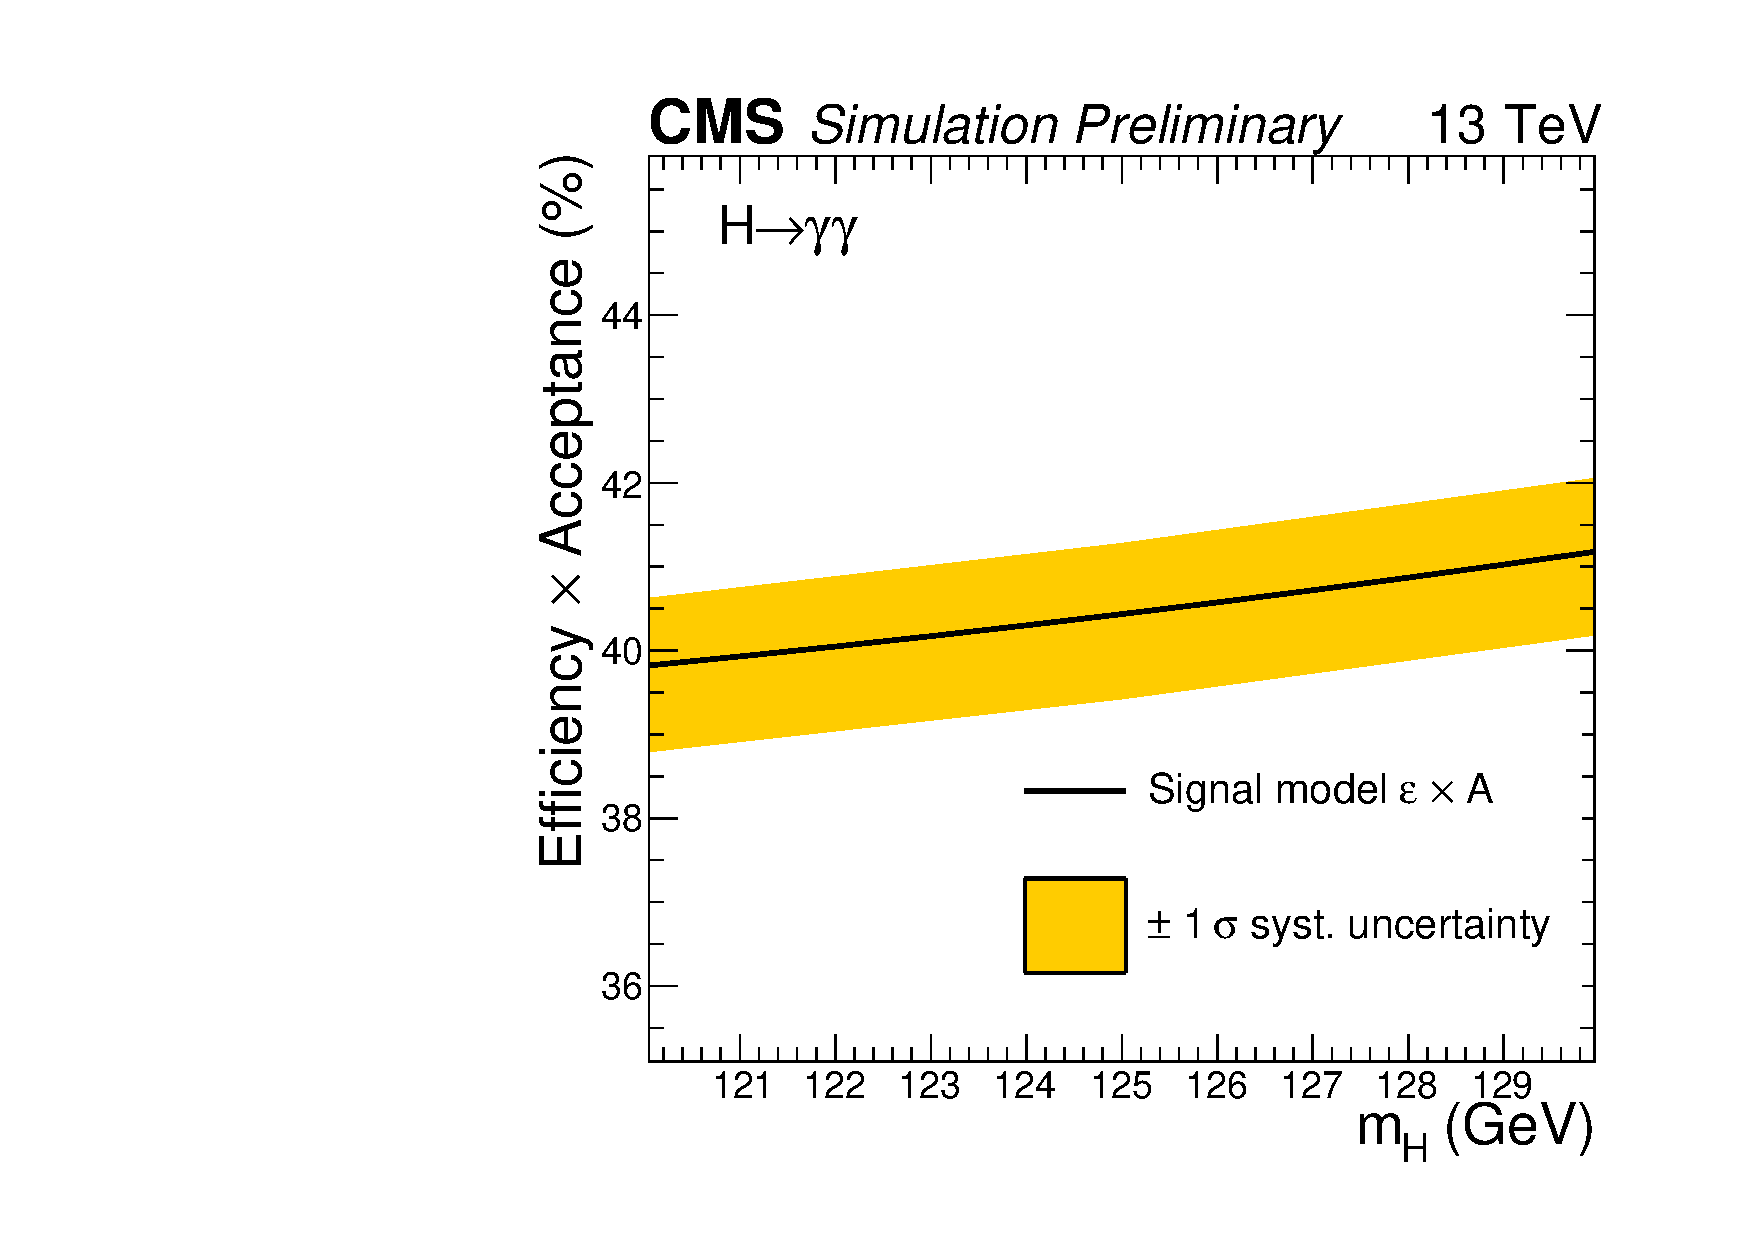
\includegraphics[width=0.6\textwidth]{modellingFigures/effAcc_vs_mass.pdf} 
\caption{The \effxacc of all categories combined shown as a function of \mH. The ornage band shows the effect of the systematic uncertainties associated with trigger efficiency, photon identification and selection, photon energy scale and resolution and vertex identification.}

\label{fig:model:sig_effxacc}
\end{figure}

The normalised signal models for each process are summed together to obtain the expected signal \mgg distribution for a given analysis category or for all categories combined, as shown in \Fig\s~\ref{fig:model:sig_model_all},~\ref{fig:model:sig_model_per_category_inc} and~\ref{fig:model:sig_model_per_category_exc}.
\begin{figure}[ht!]
\centering
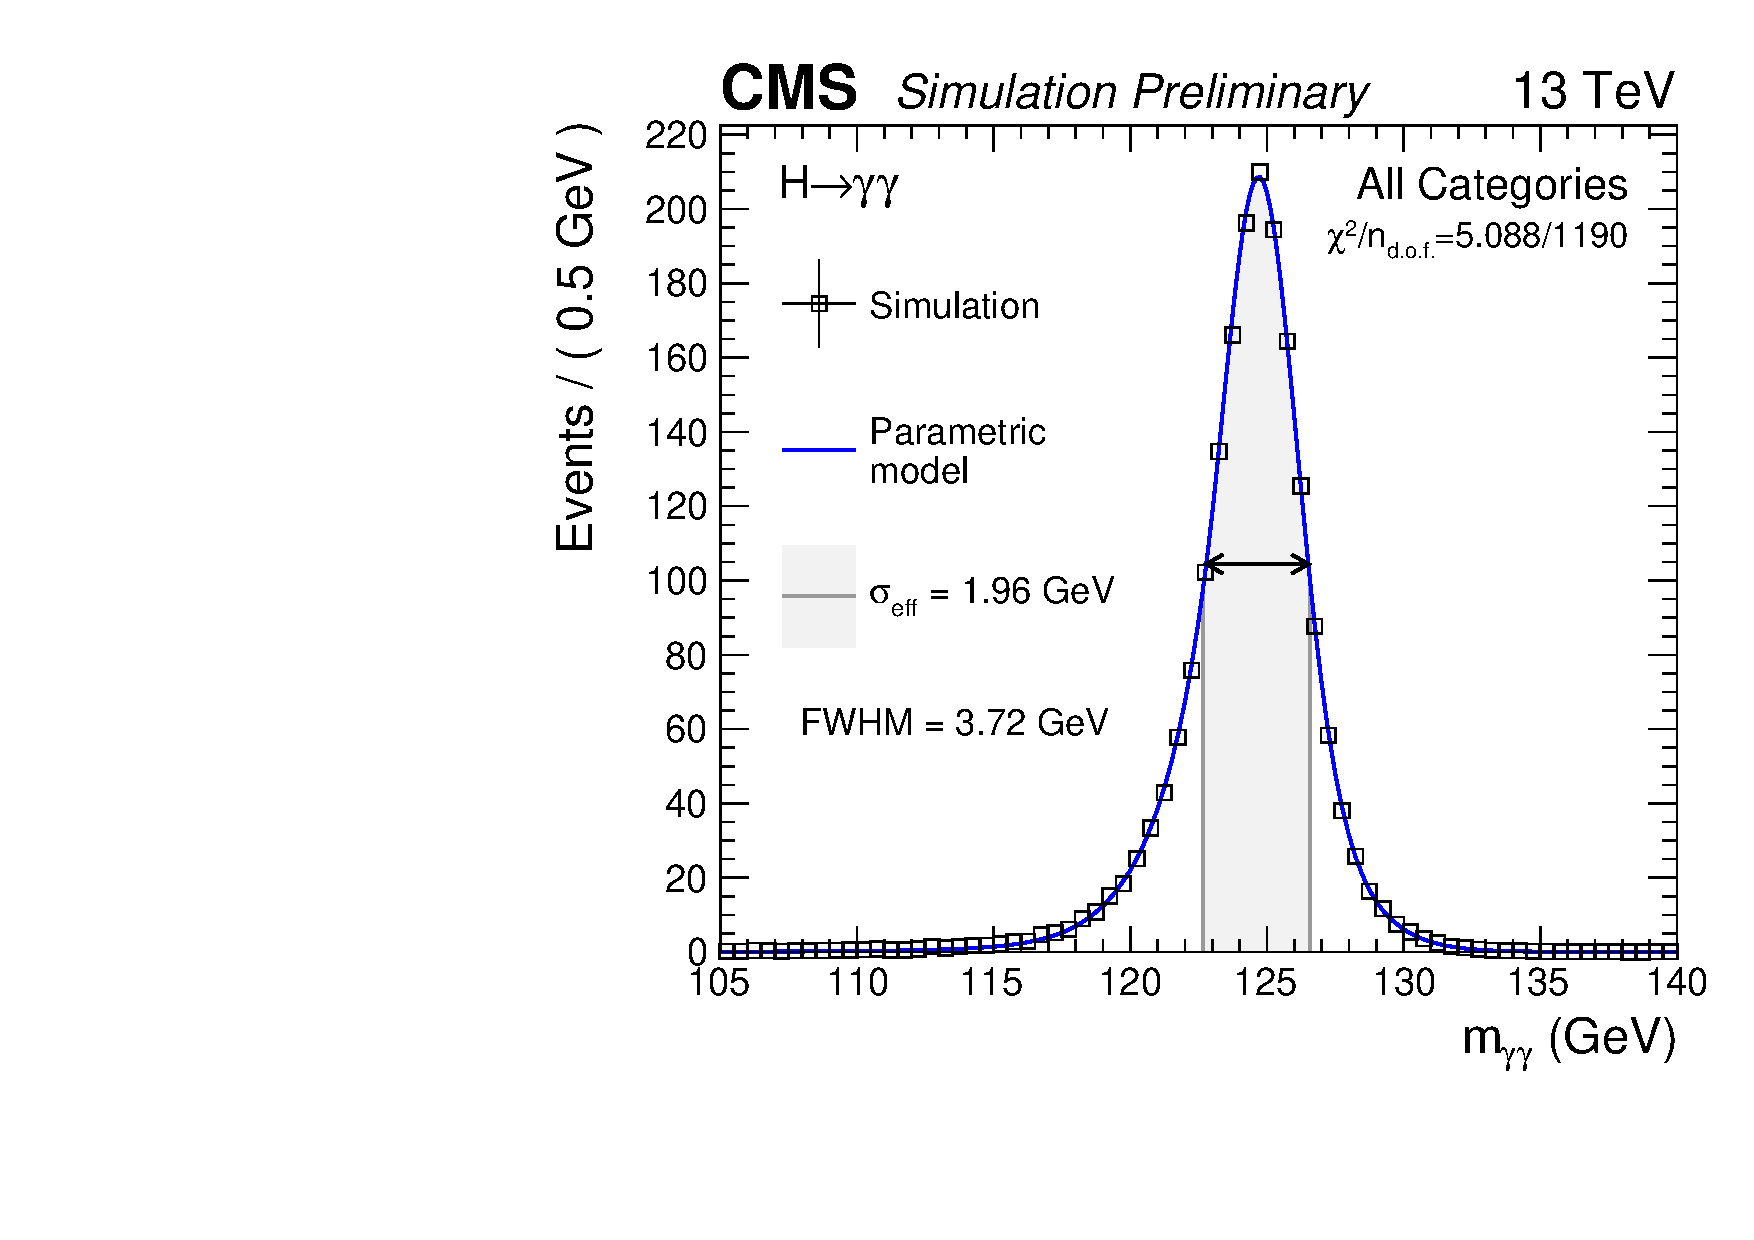
\includegraphics[width=0.6\textwidth]{modellingFigures/DCBpG/all.pdf} 

\caption{The signal model for all analysis categories combined for $\mH=125\GeV$, obtained by summing the contributions from each production process according to the \effxacc. The \effSigma value (half the width of the narrowest interval containing 68.3\% of the invariant mass distribution) and the FWHM (the width of the distribution at half of the maximum value) are also shown. }

\label{fig:model:sig_model_all}
\end{figure}

\begin{figure}[ht!]
\centering
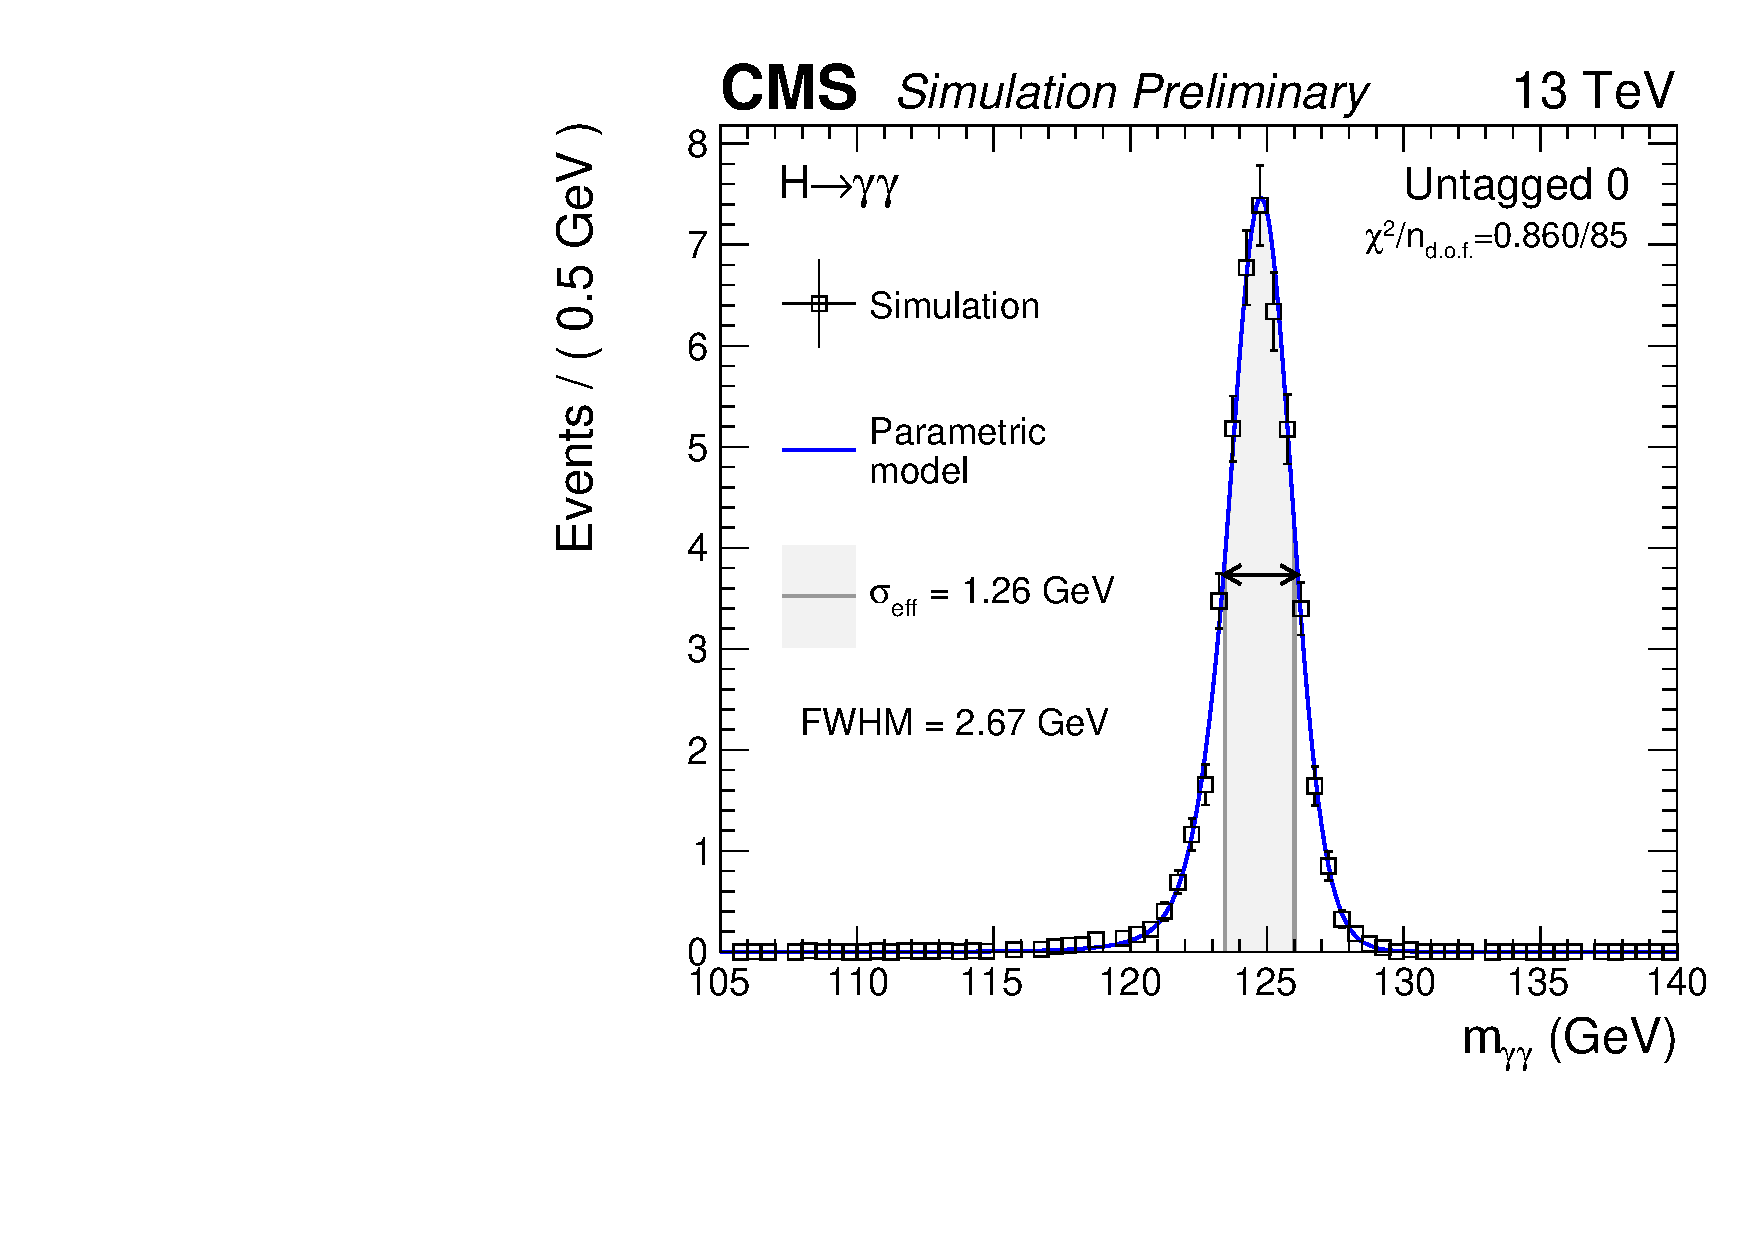
\includegraphics[width=0.45\textwidth]{modellingFigures/DCBpG/UntaggedTag_0.pdf} 
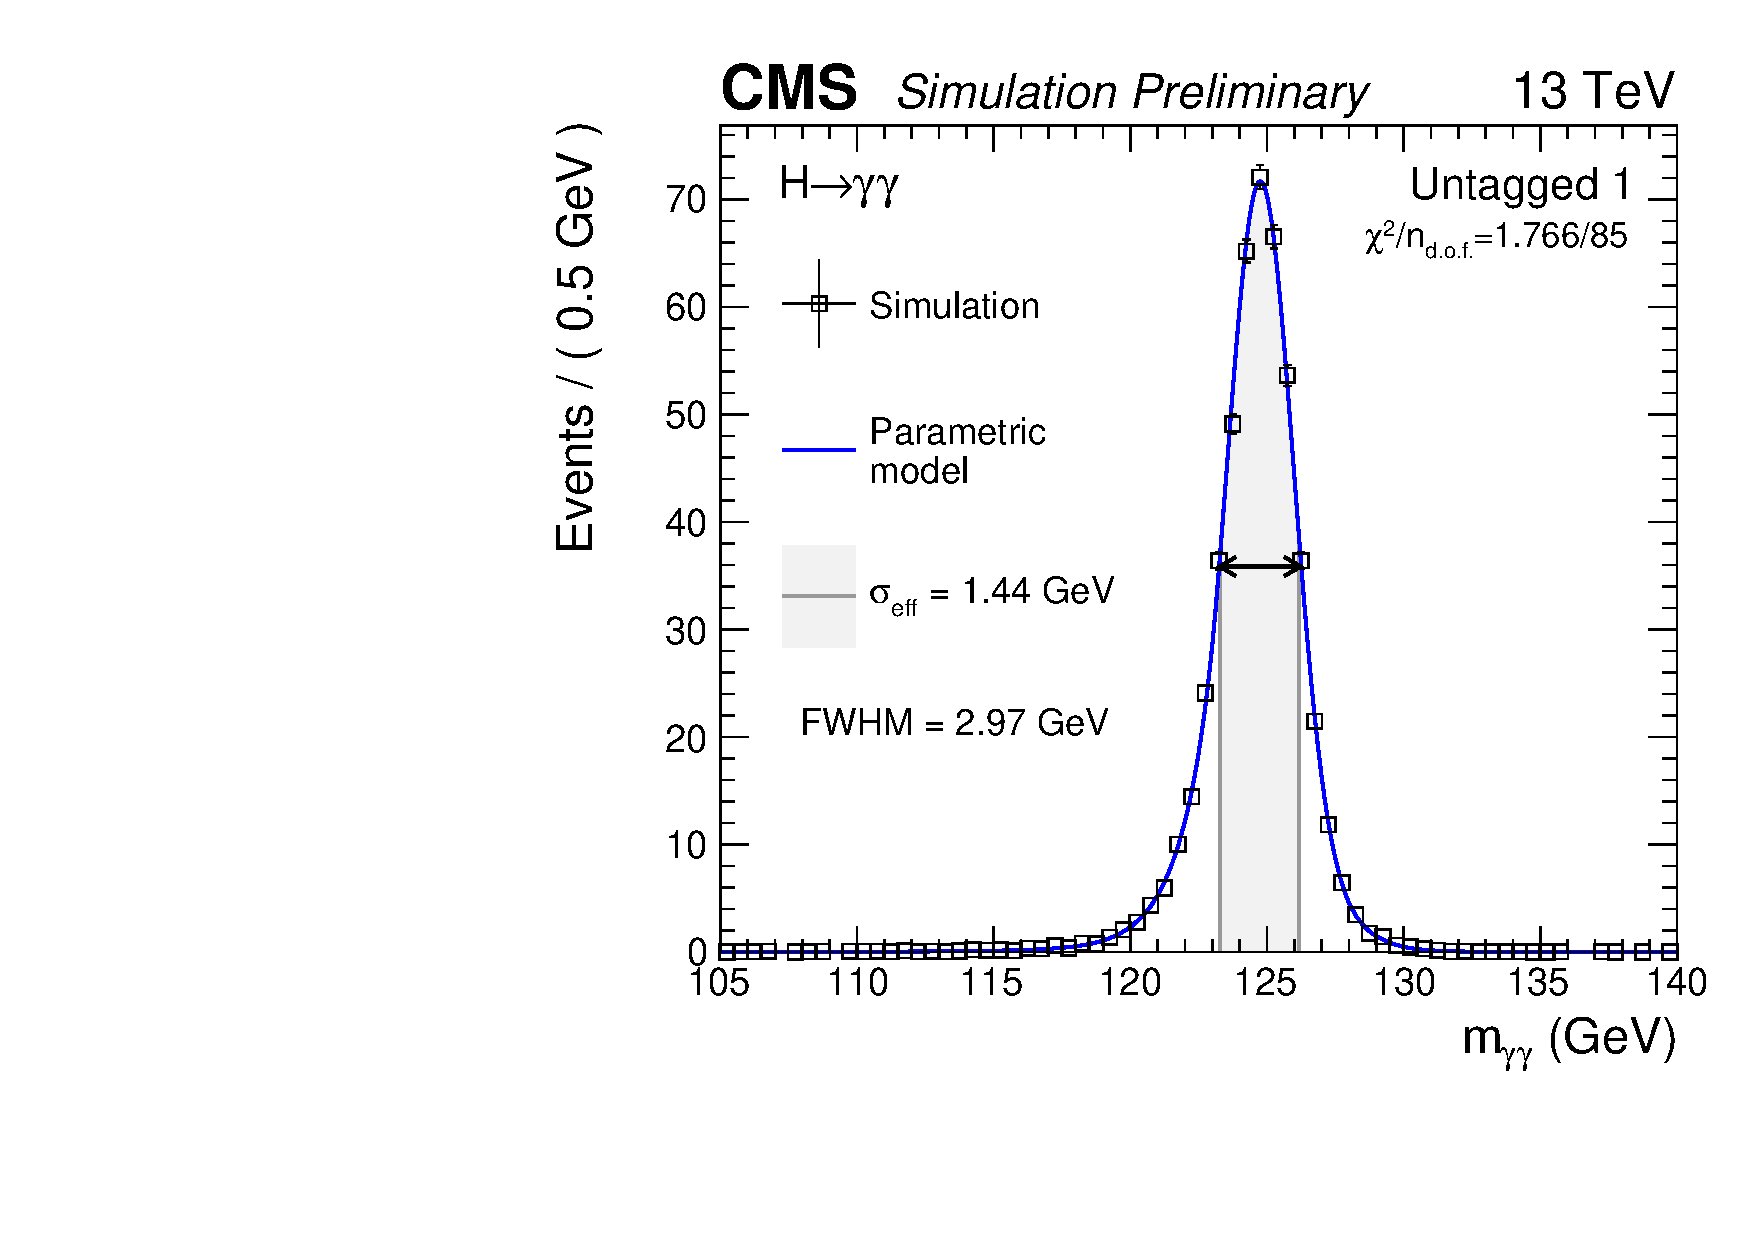
\includegraphics[width=0.45\textwidth]{modellingFigures/DCBpG/UntaggedTag_1.pdf} \\
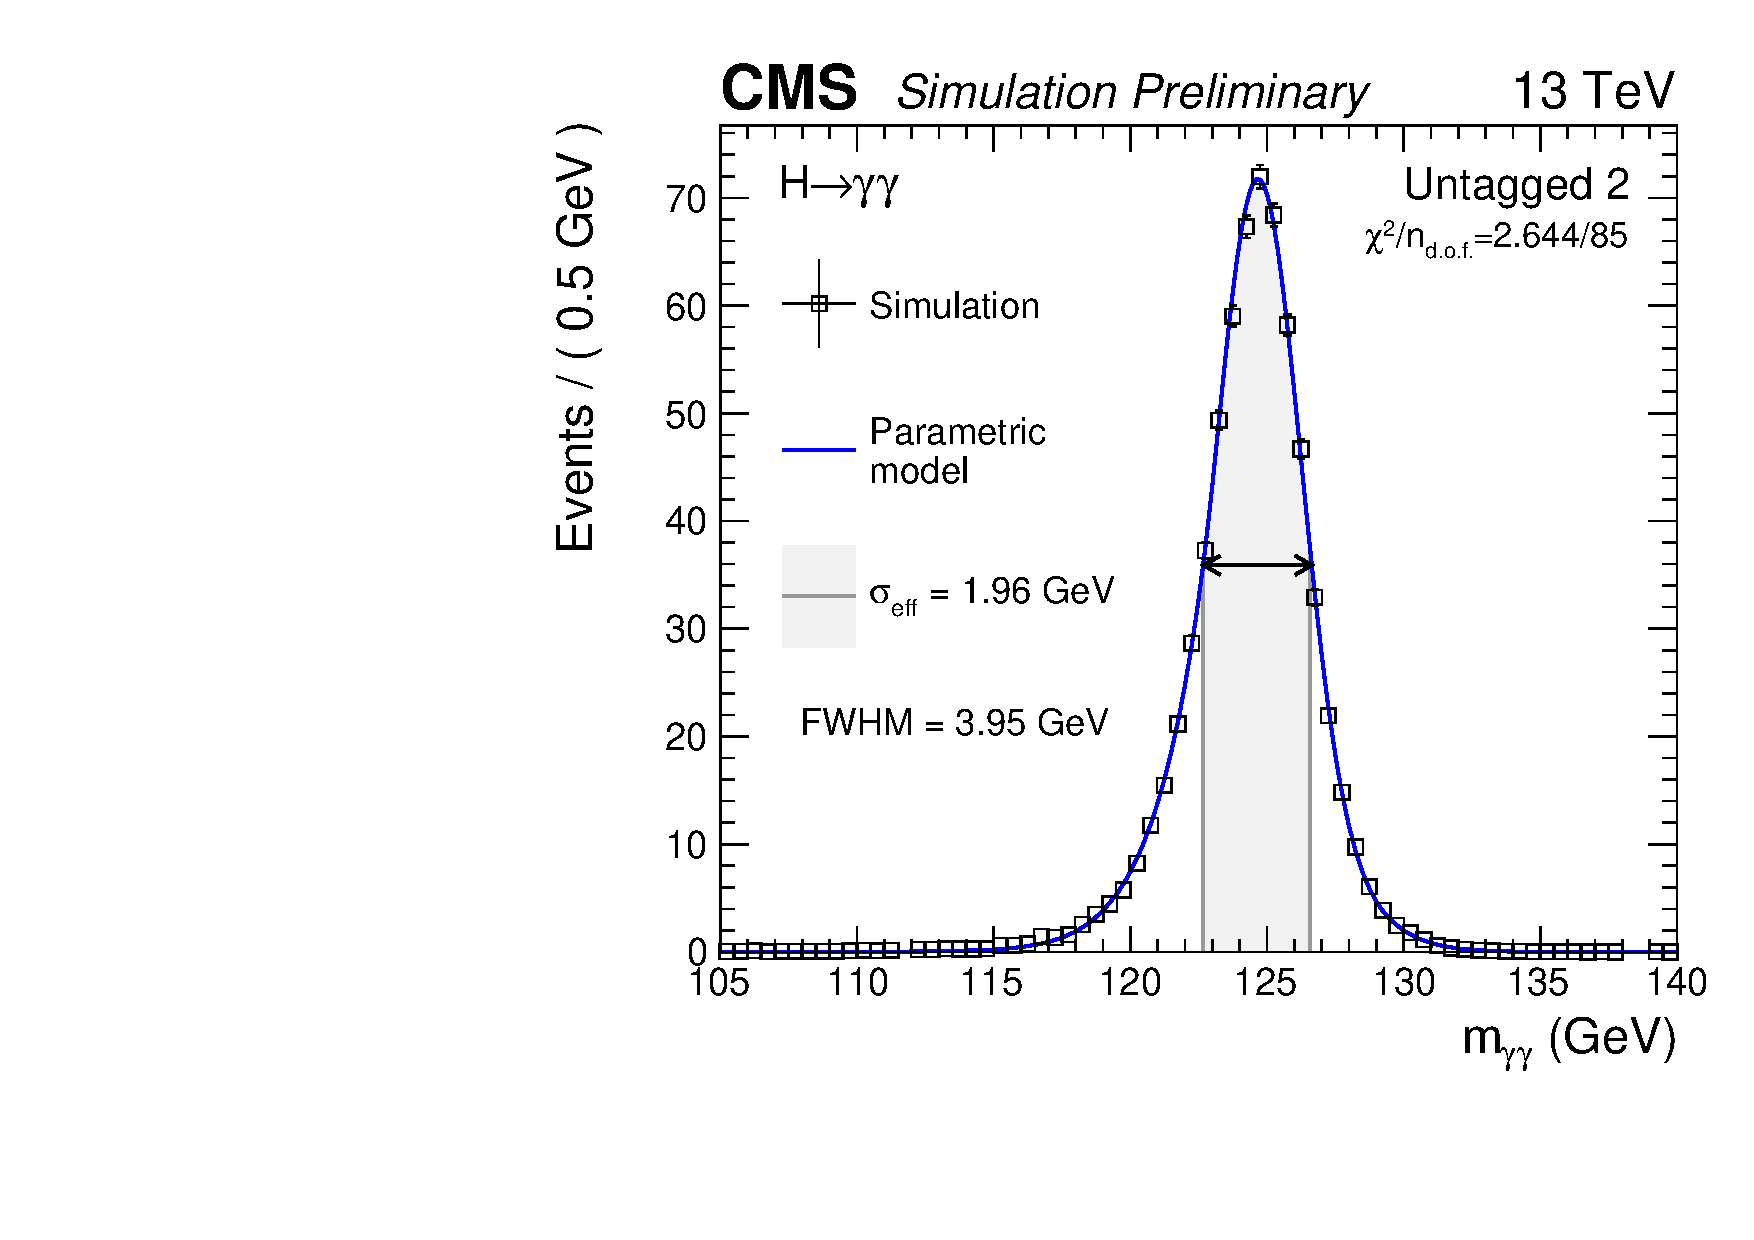
\includegraphics[width=0.45\textwidth]{modellingFigures/DCBpG/UntaggedTag_2.pdf} 
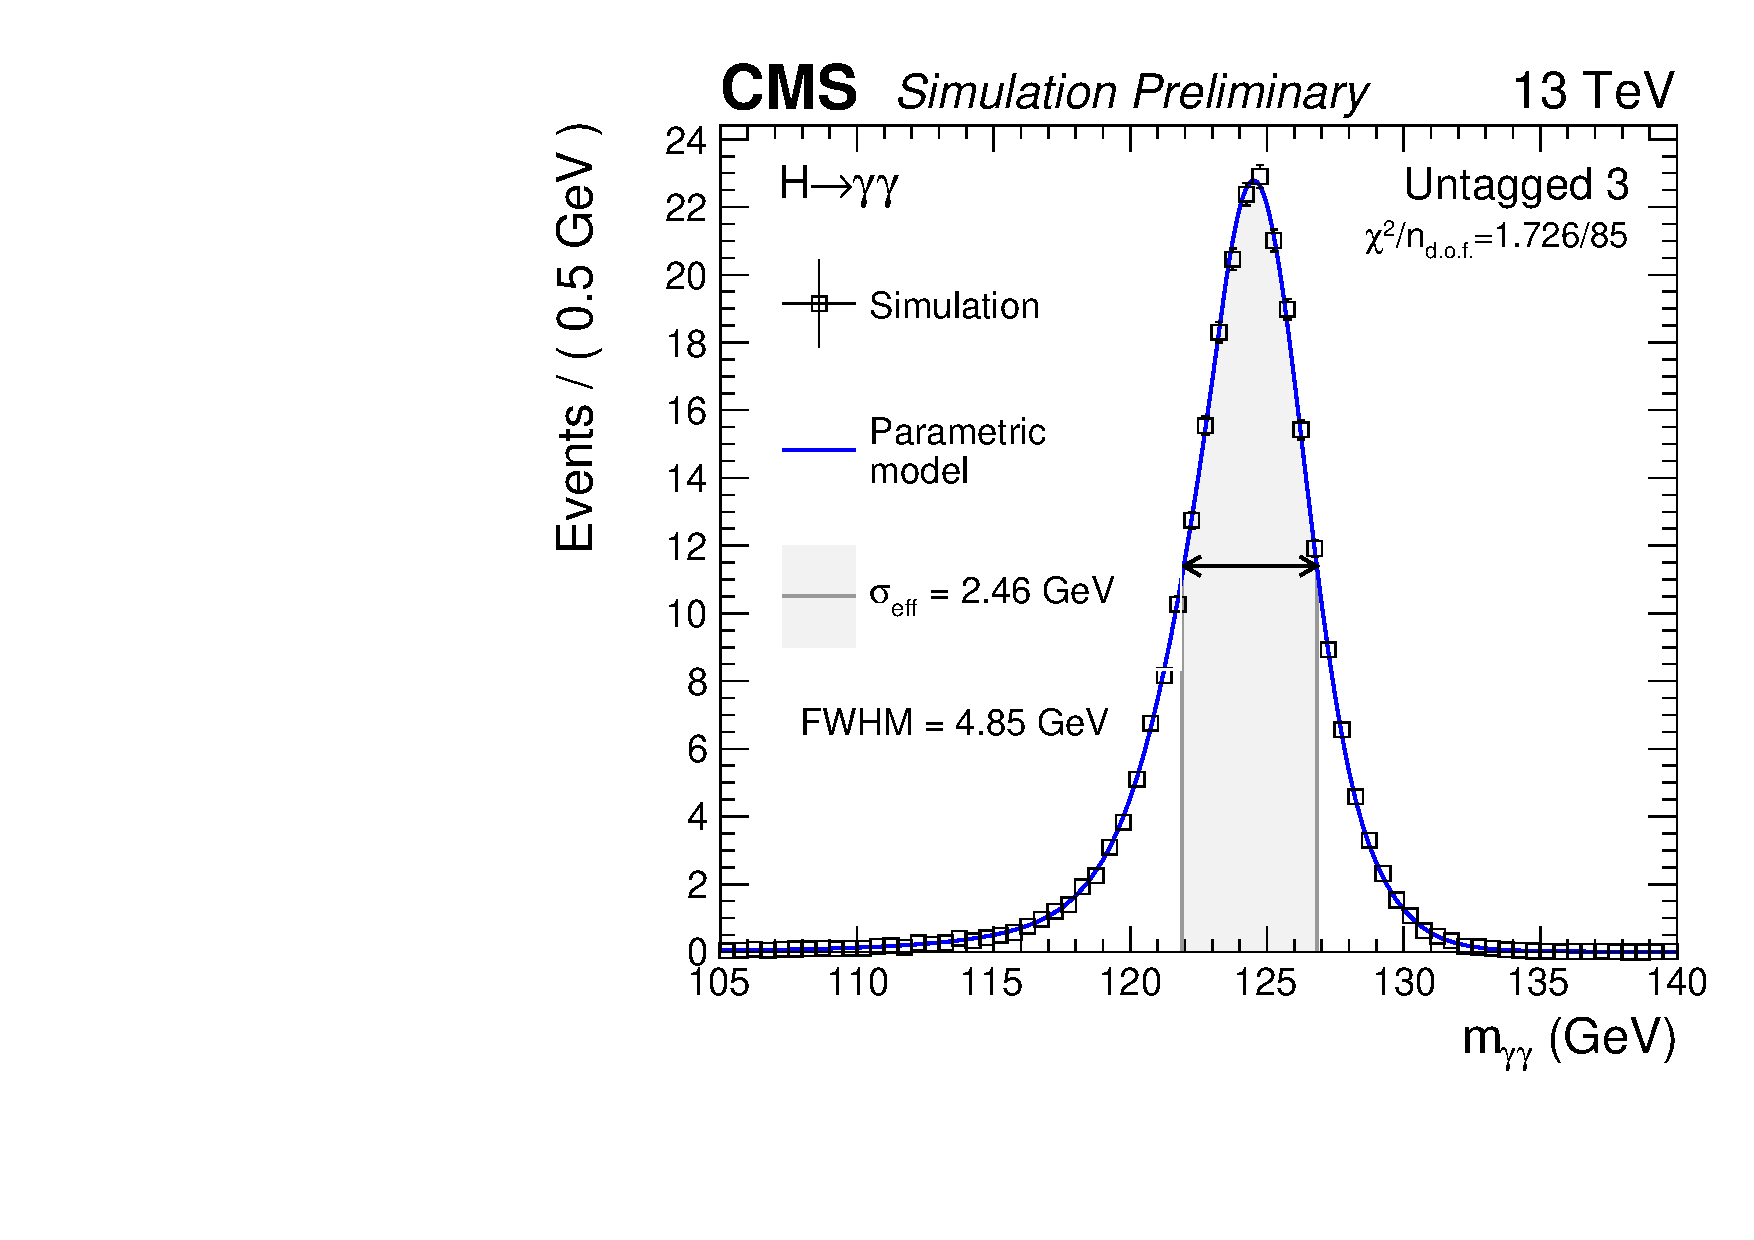
\includegraphics[width=0.45\textwidth]{modellingFigures/DCBpG/UntaggedTag_3.pdf}  

\caption{The signal models for the inclusive analysis categories for $\mH=125\GeV$, obtained by summing the contributions from each production process according to their \effxacc. The \effSigma value (half the width of the narrowest interval containing 68.3\% of the invariant mass distribution) and the FWHM (the width of the distribution at half of the maximum value) are also shown.}

\label{fig:model:sig_model_per_category_inc}
\end{figure}
\begin{figure}[ht!]
\centering
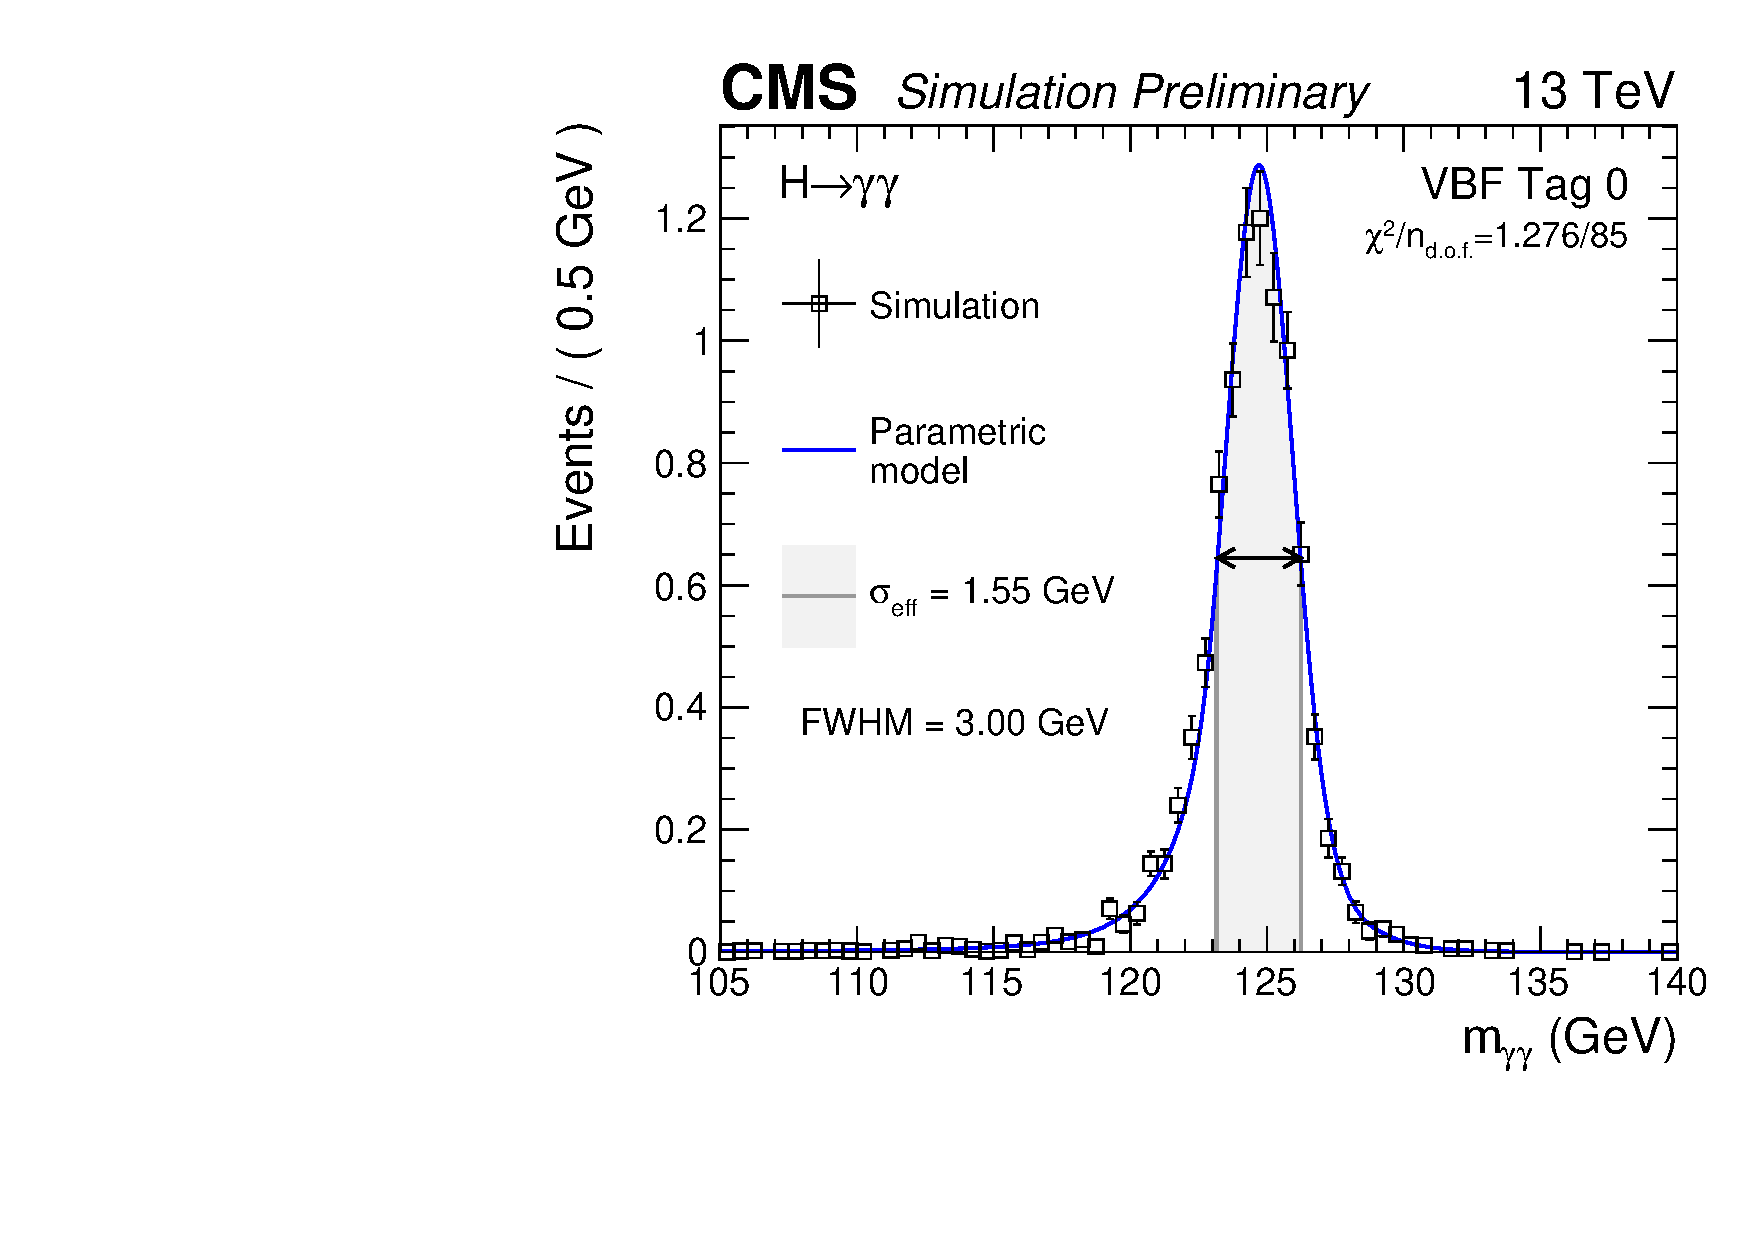
\includegraphics[width=0.45\textwidth]{modellingFigures/DCBpG/VBFTag_0.pdf} 
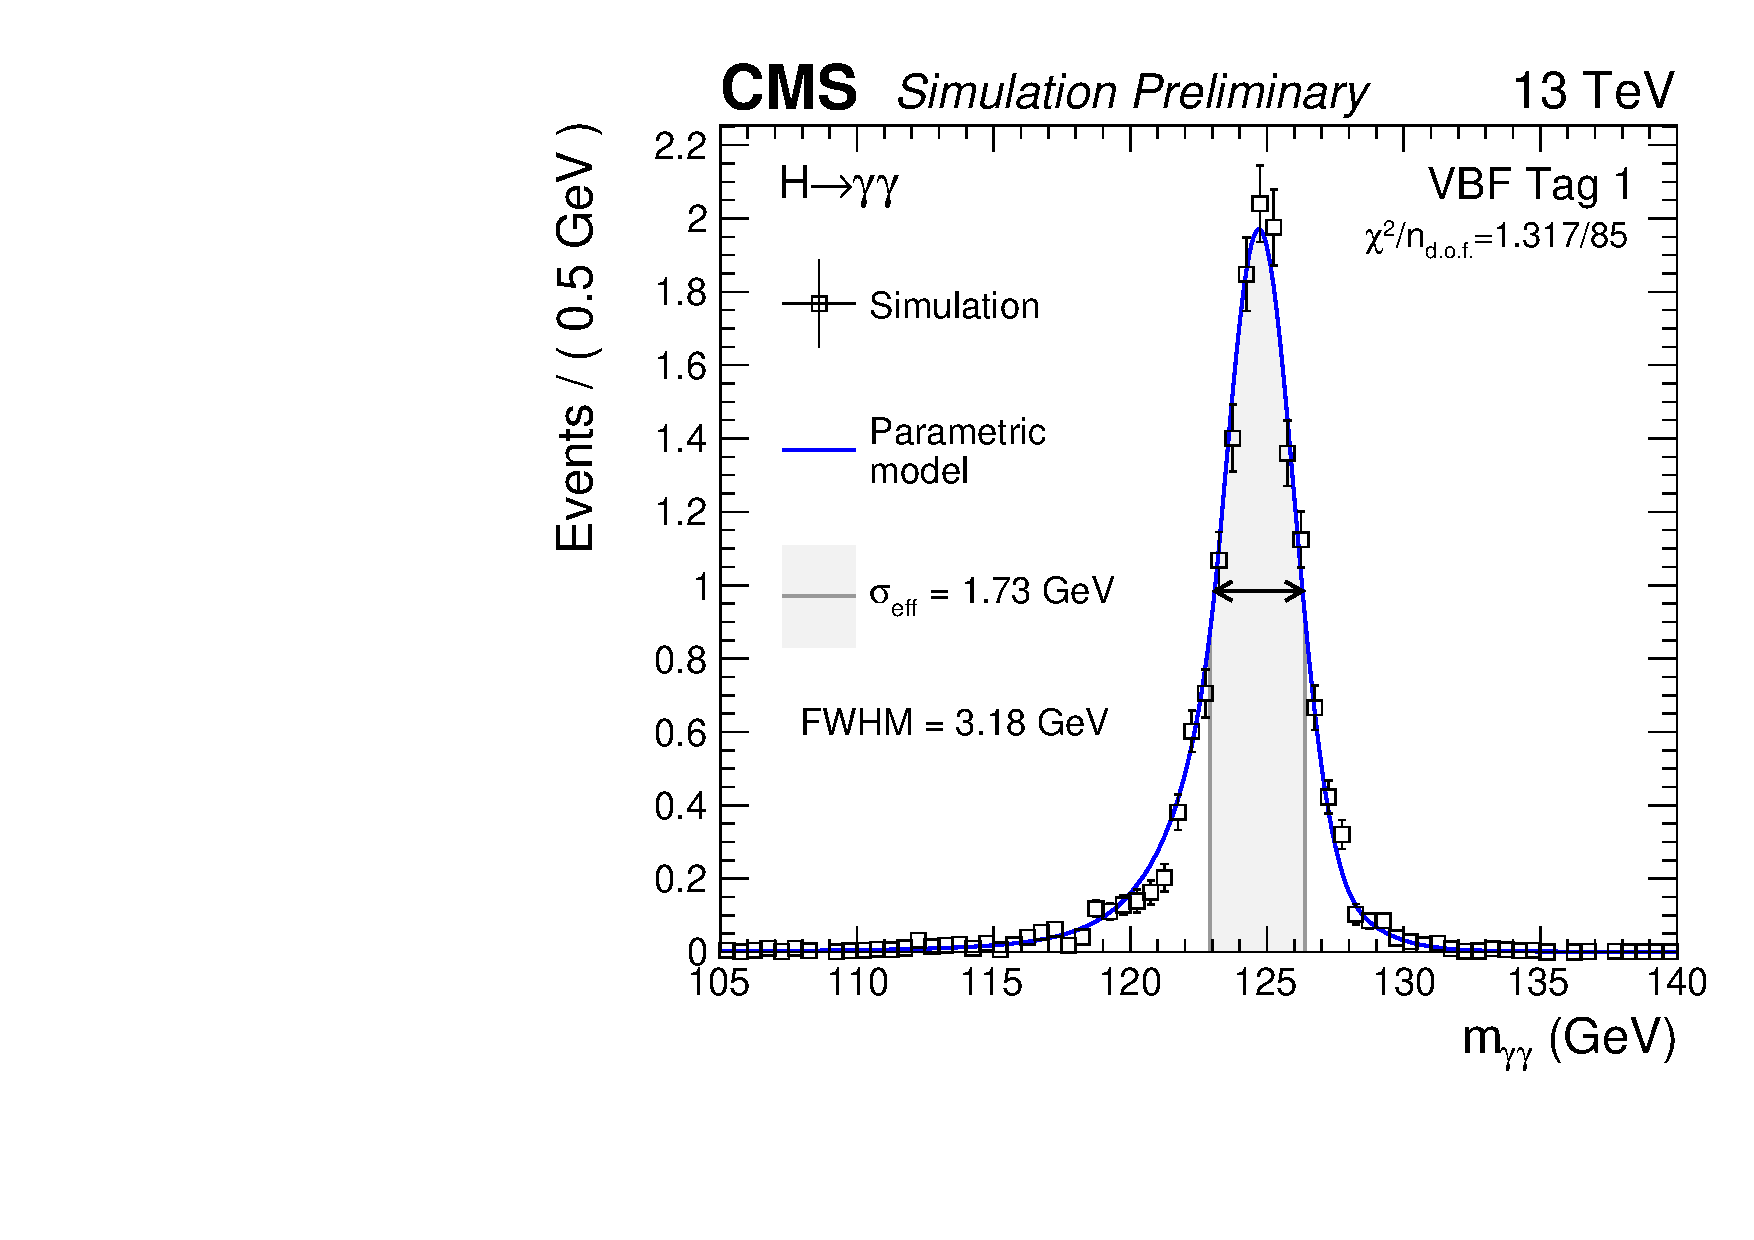
\includegraphics[width=0.45\textwidth]{modellingFigures/DCBpG/VBFTag_1.pdf} \\
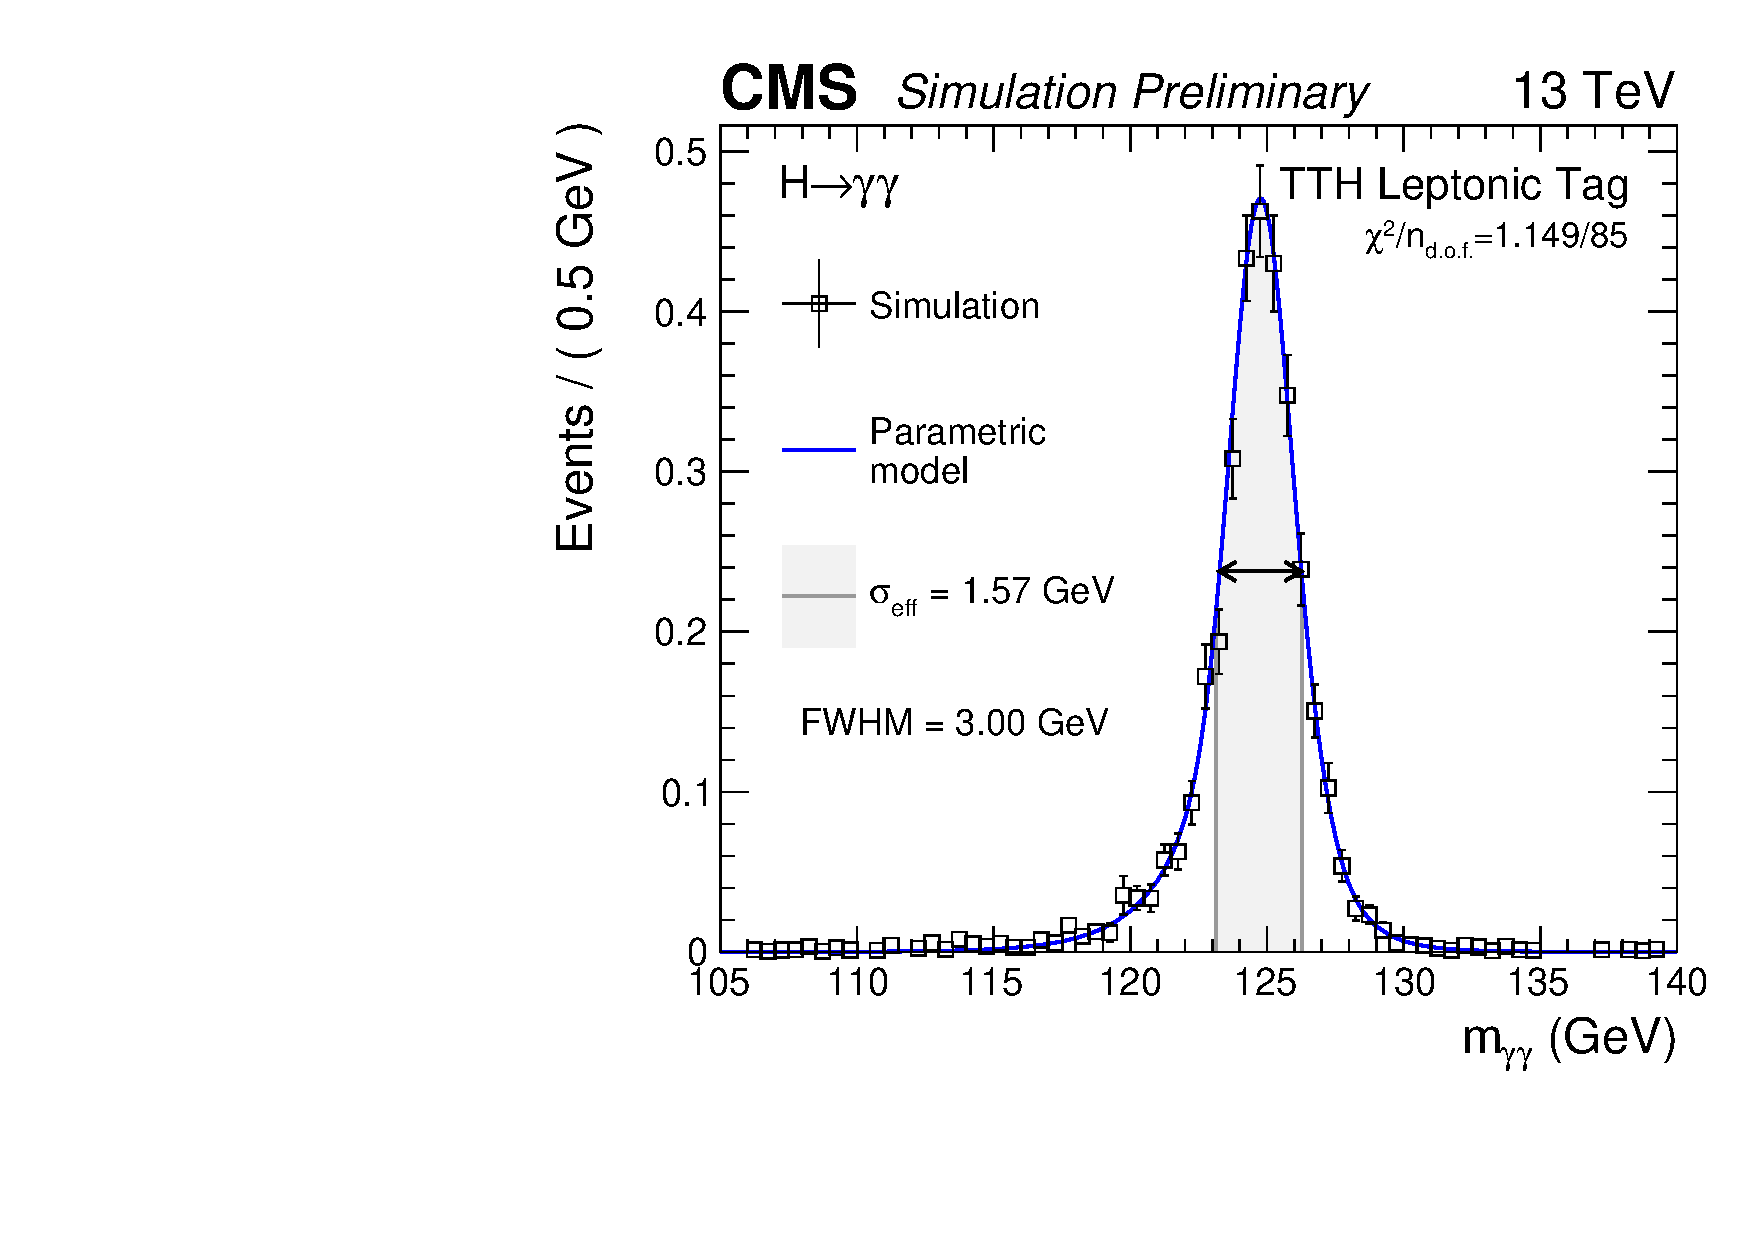
\includegraphics[width=0.45\textwidth]{modellingFigures/DCBpG/TTHLeptonicTag.pdf} 
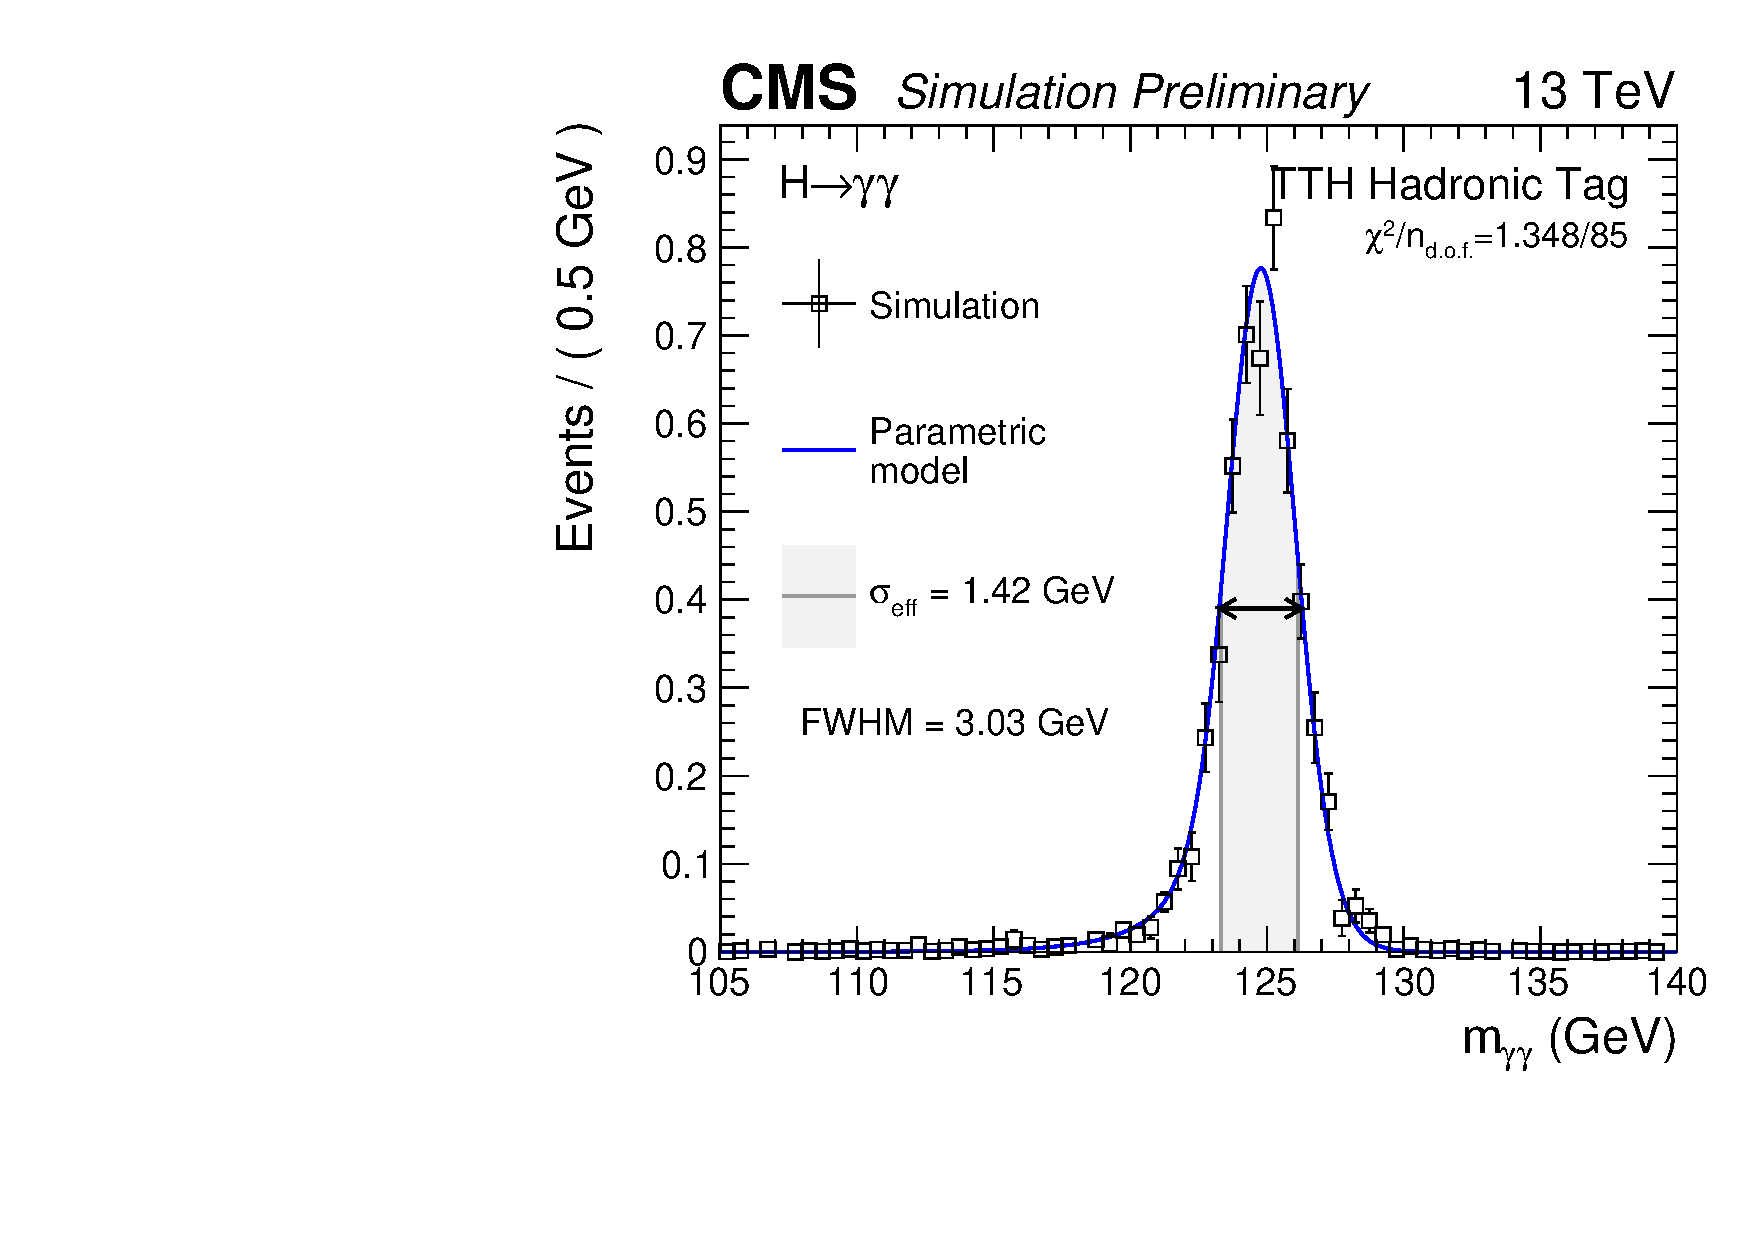
\includegraphics[width=0.45\textwidth]{modellingFigures/DCBpG/TTHHadronicTag.pdf} 

\caption{The signal models for the \VBFTag and \TTHTag analysis categories for $\mH=125\GeV$, obtained by summing the contributions from each production process according to their \effxacc. The \effSigma value (half the width of the narrowest interval containing 68.3\% of the invariant mass distribution) and the FWHM (the width of the distribution at half of the maximum value) are also shown.}

\label{fig:model:sig_model_per_category_exc}
\end{figure}



%\subsection{Handling of photon energy systematics}

%The systematics associa

\section{Background modelling}
\label{model:sec:background_model}
\subsection{The discrete profiling method}

The background model is produced from data using the discrete profiling method~\cite{DiscreteProfiling}, which treats the choice of functional form to describe the background as a discrete nuisance parameter in the final \NLL fit to the data. 

The underlying functional form of a given background distribution is typically not known. In some cases, several different families of function could in principle be chosen to parametrise the background distribution, all giving acceptable agreement with the data. Even within a given family of functions, it is not always clear which order to choose. Furthermore, the uncertainty associated with making a particular choice must be accounted for. %An common solution is to make an arbitrary choice of functional form and try to estimate the bias introduced by pikcing that shape, and trying to assign some systematic uncertainty to compensate.
The discrete profiling method avoids an arbitrary choice and provides a natural way to handle the uncertainty due to the background parametrisation.

When making a measurement of a parameter of interest using a \NLL minimisation, nuisance parameters representing systematic uncertainties are typically profiled: they are allowed to float during the minimisation, but their final value is not of interest. The additional freedom produces a wider \NLL curve, representing the additional uncertainty attributed to the nuisances. 
If the value of one of the nuisance parameters is instead fixed at the best-fit value, the width of the resulting \NLL curve will be narrower but still with its minimum at the same place as the full profiled \NLL curve. This width represents the uncertainty of the measurement without the effect of the fixed nuisance parameter. If the procedure is repeated for different fixed values of the nuisance parameter, different \NLL curves, not necessarily at the minimum, will be produced. In the limit that many different values of the fixed nuisance parameter are sampled, the minimum envelope of all the fixed-nuisance \NLL curves will converge to the full profiled \NLL curve. The uncertainty can then be obtained from the envelope as for a usual \NLL curve. This property is true also for discrete nuisance parameters. This procedure is illustrated in \Fig~\ref{fig:model:bkg_envelope}. When parametrising the background distribution, since the chosen functional form itself is not of interest, it can be treated as a discrete nuisance parameter. The method described above can then be used to account for the uncertainty associated with the parametrisation of the background. The fact that different functional forms can have different numbers of degrees of freedom is taken into account by adding a penalty term to the \NLL proportional to the number of parameters in the functional form. 

\begin{figure}[ht!]
\centering
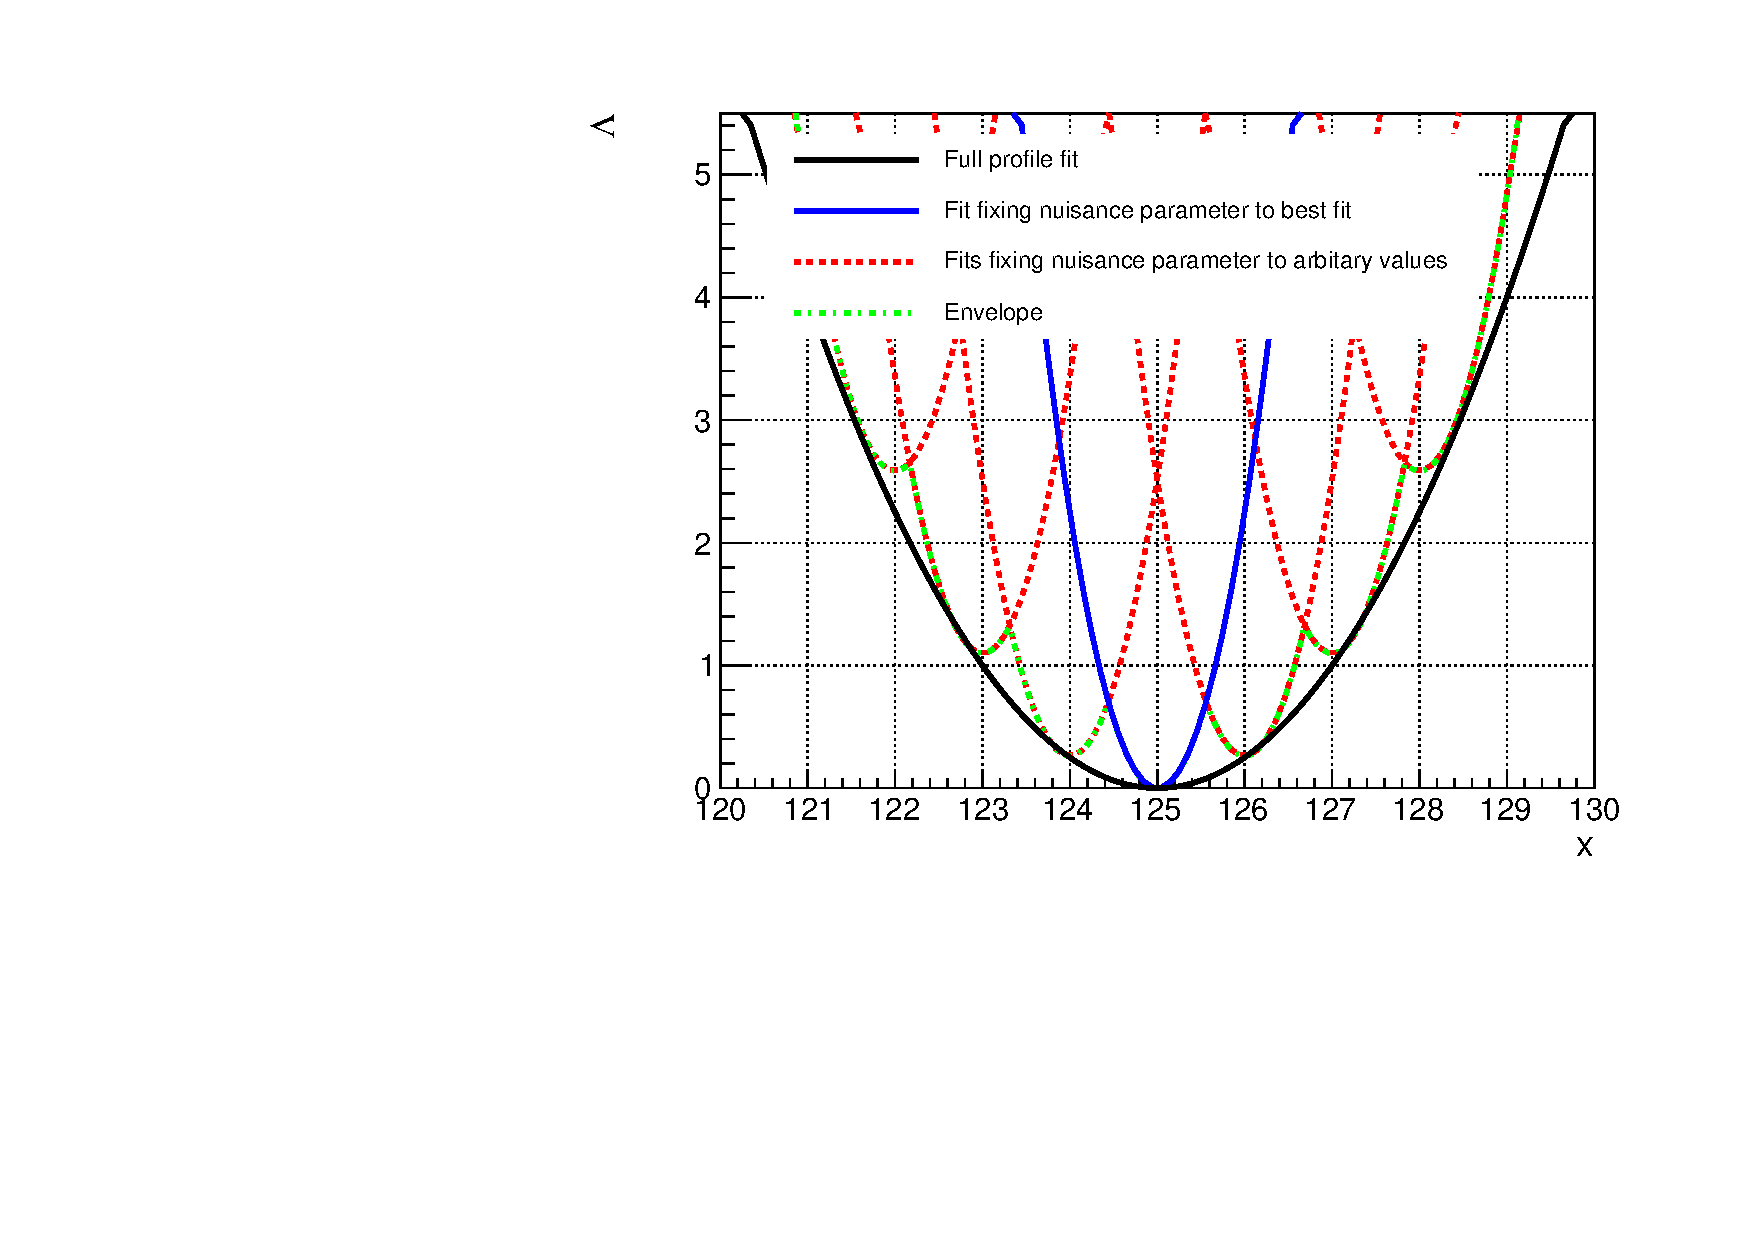
\includegraphics[width=0.8\textwidth]{modellingFigures/envelope_cartoon.pdf} 
\caption{An illustration of the construction of the envelope to estimate the effect of a nuisance parameter. The NLL (denoted as $\Lambda$) curve obtained when performing a likelihood scan of parameter of interest $x$ if the nuisance parameter is profiled is shown in black. The NLL curve obtained by fixing the nuisance to the best-fit value is shown in blue. The NLL curves for various fixed values of the nuisance other than the best-fit are shown in red. The minimum envelope of these curves, shown in green, approximates the original NLL curve obtained by profiling the nuisance parameter~\cite{DiscreteProfiling}.}

\label{fig:model:bkg_envelope}
\end{figure}

A complete set of all analytic functions should be considered to obtain an exact result using the discrete profiling method. In practice, it is only necessary to include the subset of all analytic function which give a good description of the data. In this analysis, the following four families of functions are considered:

\begin{itemize}
\item Sums of exponentials: $$ f_{N}(x)= \sum^{N}_{i=1} p_{2i} e^{p_{2i+1} x} ,$$
\item Sums of polynomials (in the Bernstein basis): $$ f_{N}(x) = \sum^{N}_{i=0} p_{i} b_{(i,N)}, \text{ where } b_{(i,N)}:= \begin{pmatrix} N \\ i \end{pmatrix} x^i (1-x)^{N-i} ,$$
\item Laurent series: $$ f_{N}(x)= \sum^{N}_{i=1} p_{i} x^{-4 + \sum^{i}_{j=1} (-1)^{j} (j-1)},$$
\item Sums of power-law functions: $$ f_{N}(x)= \sum^{N}_{i=1} p_{2i} x^{-p_{2i+1}},$$
\end{itemize}
where for all $k$, the $p_k$ are a set of parameters, and $N$ represents the order of a particular function in the family.  

%The representations of the function families are chosen such that their members are nested: a function of a particular order can reproduce the shape of the functions of lower order for a suitable choice of parameter values. It is therefore only necessary to consider a single representative function from each family when applying the discrete profiling method. 
The maximum order of the candidate function from each family is obtained separately for each analysis category using the following procedure. Starting with the lowest-order function in the family, the parameters of the candidate function are varied to minimize the \NLL with respect to the $m_{\gamma\gamma}$ distribution. A penalty of 0.5 times the number of parameters in the functional form is added to the value of the \NLL to account for differences in the number of degrees of freedom. The same procedure is applied to the function of next-highest order in the family. 
In the limit of large sample size, the difference in the \NLL between functions of successive orders $N$ and $N+1$, $2 \Delta NLL_{N+1} = 2(NLL_{N+1} - NLL_{N})$, is distributed as a $\chi^2$ with $M$ degrees of freedom where, $M$ is the difference in the number of free parameters in the order-($N+1$)  and order-$N$ functions. A p-value is then calculated as:

$$ \text{p-value} = \text{prob}(2 \Delta NLL > 2 \Delta NLL_{N+1}| \chi^2(M)). $$

If the p-value is less than a predetermined threshold, chosen as $0.05$, the higher-order function is supported by the data, otherwise the higher-order function is assumed too flexible given the data. In the former case, the next-highest order function is then considered, an so on. Otherwise, the procedure terminates having found the highest-order suitable function.  An additional constraint is applied to remove low order functions which do not fit the data well. The remaining functions from each of the four families are added to the final set of candidate functions to be used in the discrete profiling, which are shown for each category in \Fig\s~\ref{fig:model_bkg)multipdf_inc} and~\ref{fig:model:bkg_multipdf_exc}.

A series of tests demonstrated that this method provides good coverage of the uncertainty associated with the choice of the function and provides an unbiased estimate of the signal strength. These tests are described in detail in~\cite{DiscreteProfiling}. 

\begin{figure}
 \begin{center}
 \subfloat[\Untagged 0]{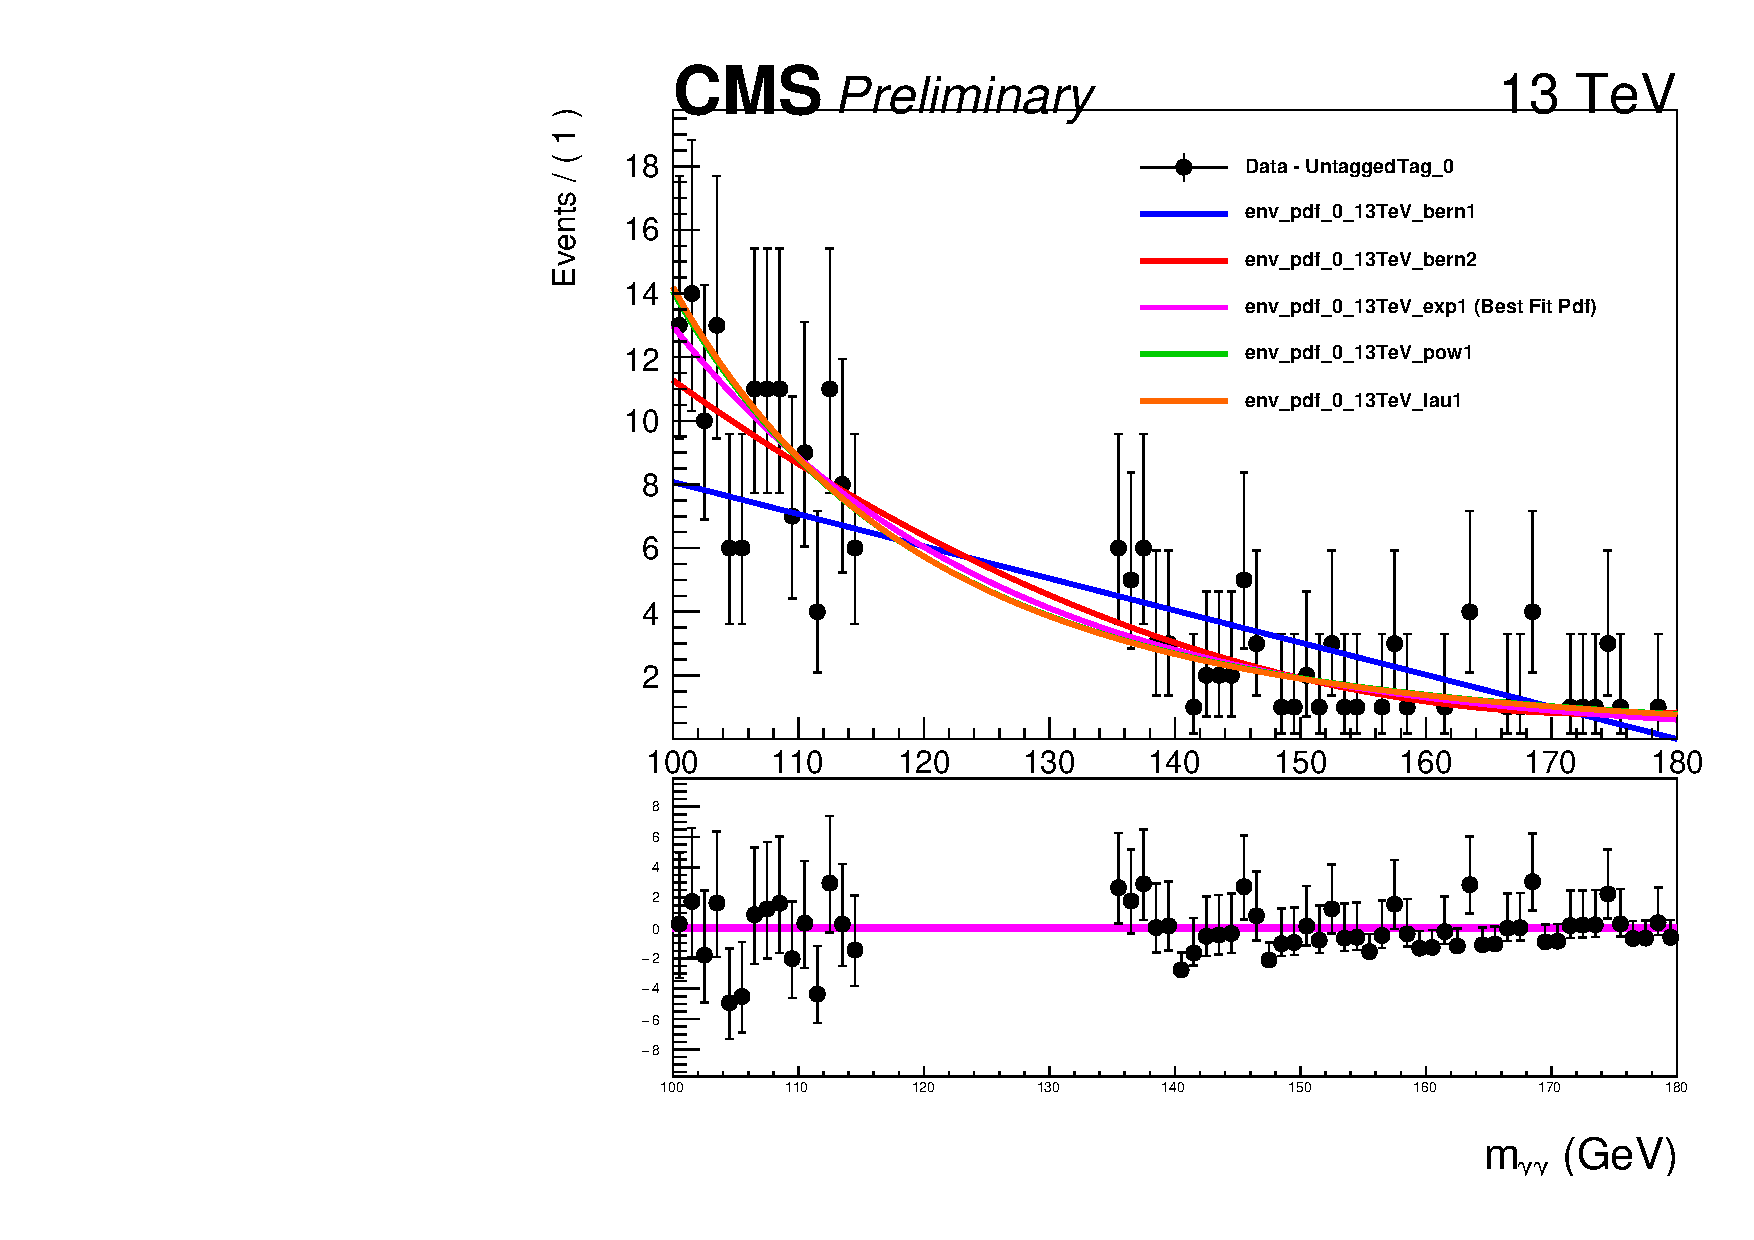
\includegraphics[width=0.48\textwidth]{modellingFigures/multipdf/multipdf_UntaggedTag_0.pdf}}
 \subfloat[\Untagged 1]{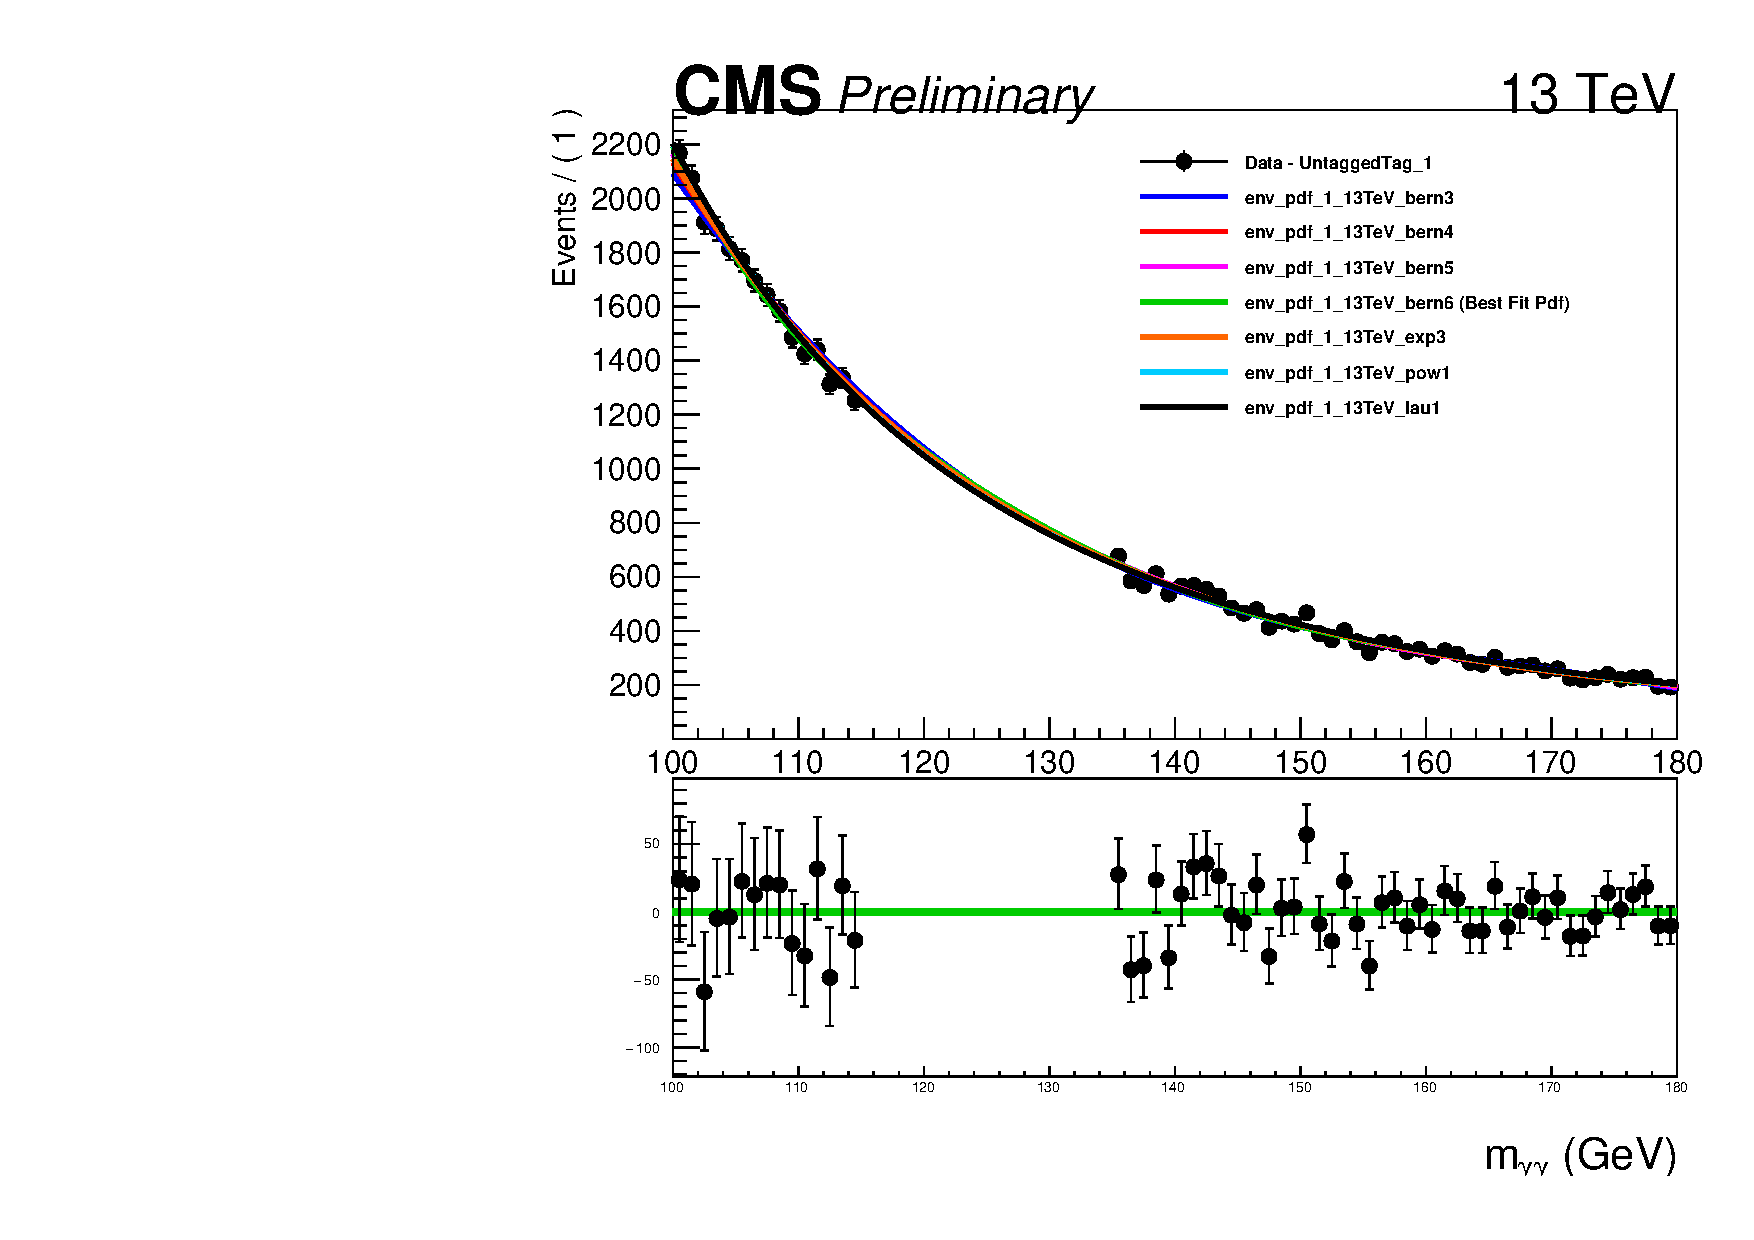
\includegraphics[width=0.48\textwidth]{modellingFigures/multipdf/multipdf_UntaggedTag_1.pdf}}\\
 \subfloat[\Untagged 2]{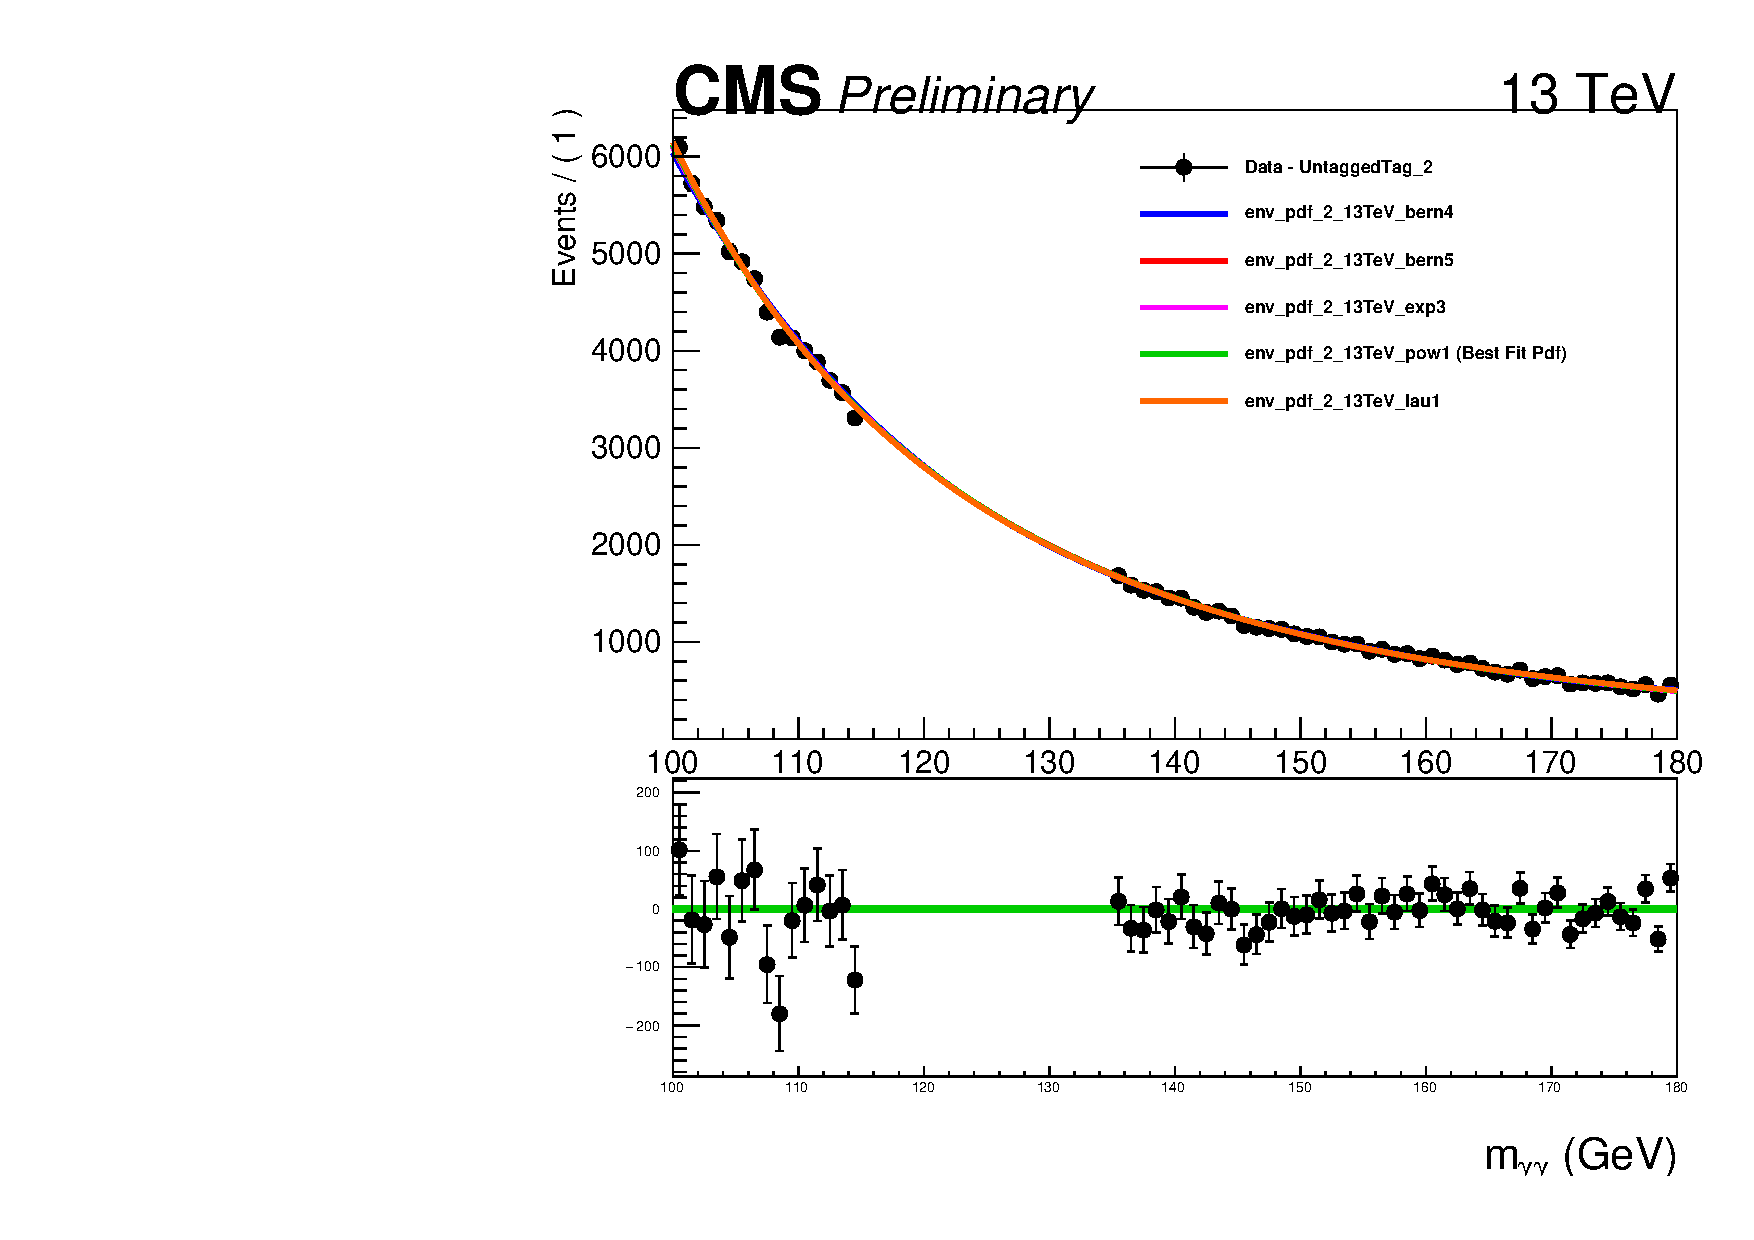
\includegraphics[width=0.48\textwidth]{modellingFigures/multipdf/multipdf_UntaggedTag_2.pdf}}
 \subfloat[\Untagged 3]{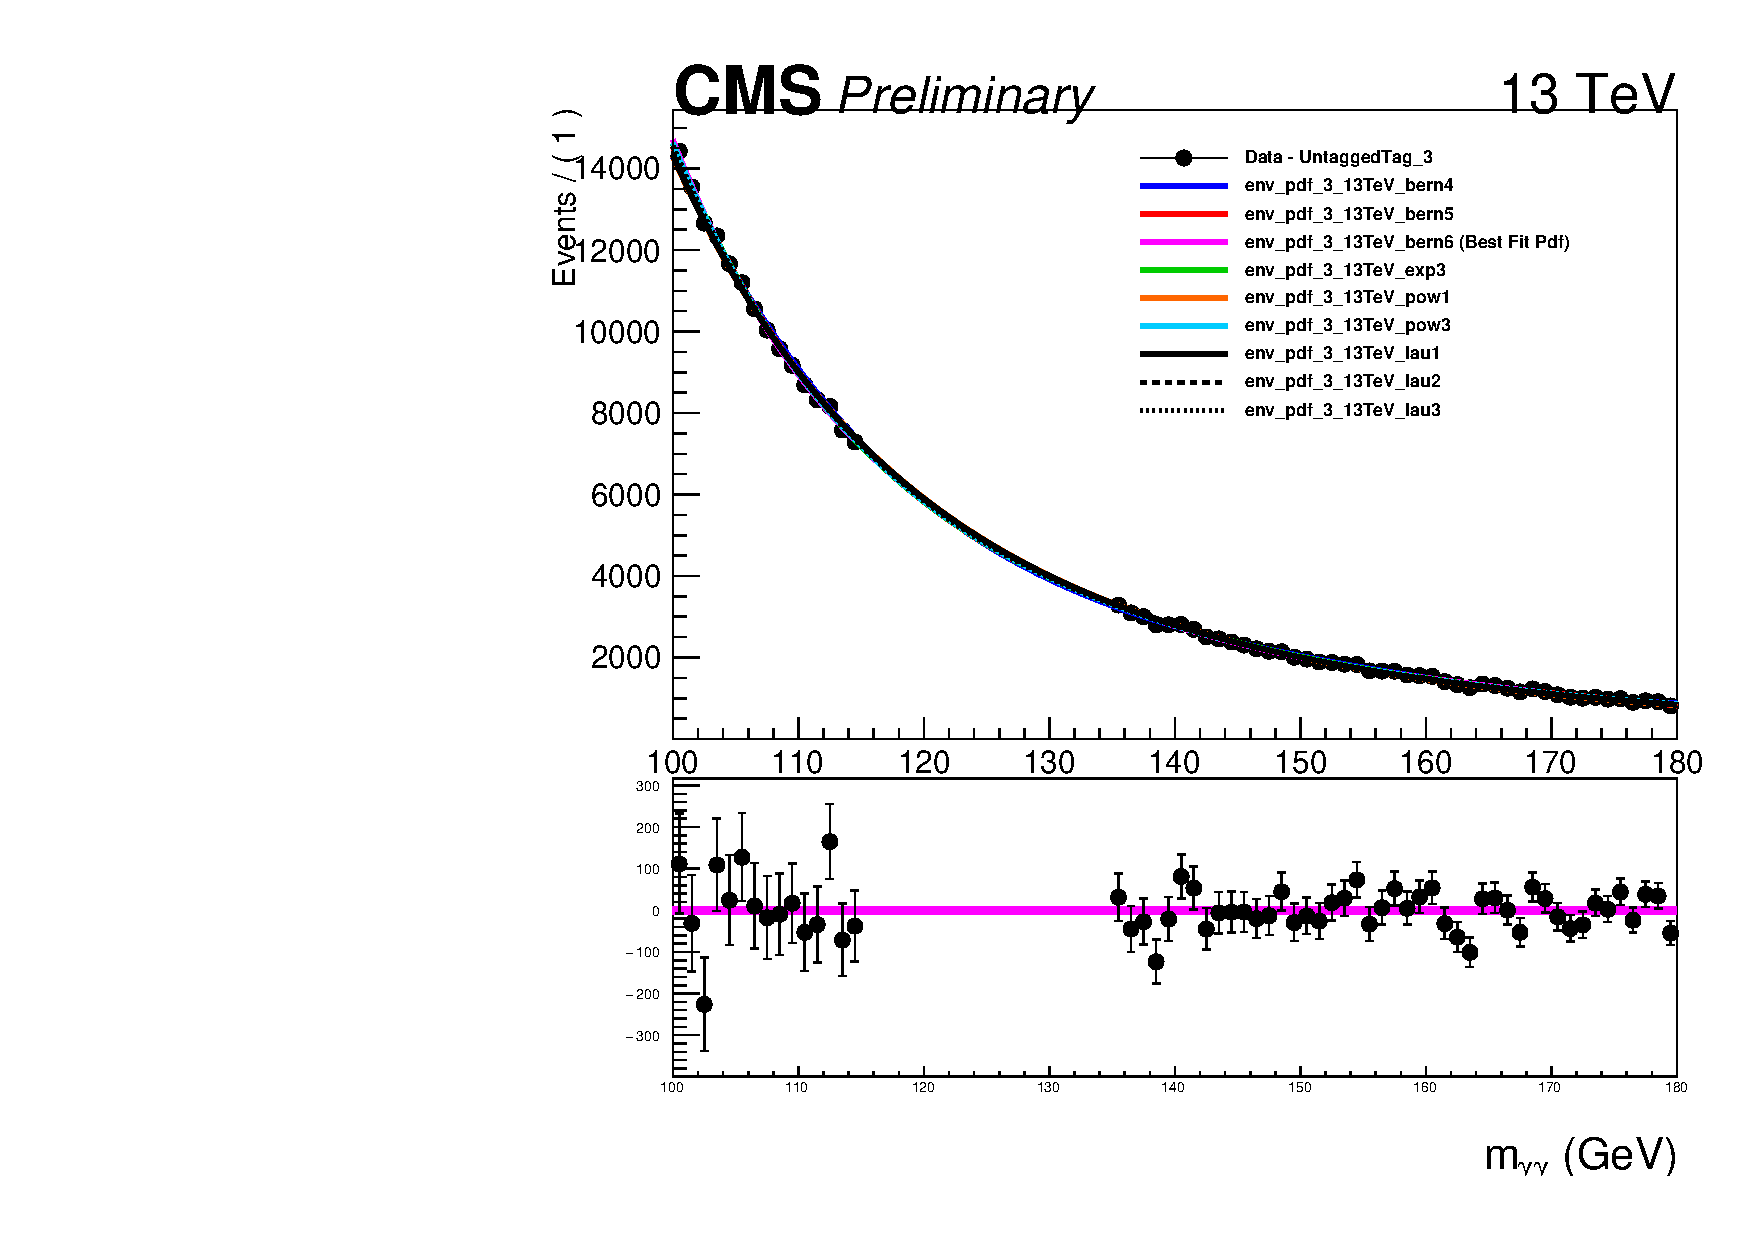
\includegraphics[width=0.48\textwidth]{modellingFigures/multipdf/multipdf_UntaggedTag_3.pdf}}\\
 \caption{The set of candidate functions chosen to parametrise the background using the discrete profiling method in the inclusive categories.}
 \label{fig:model_bkg)multipdf_inc}
 \end{center}
\end{figure}

\begin{figure}
 \begin{center}
 \subfloat[\VBFTag 0]      {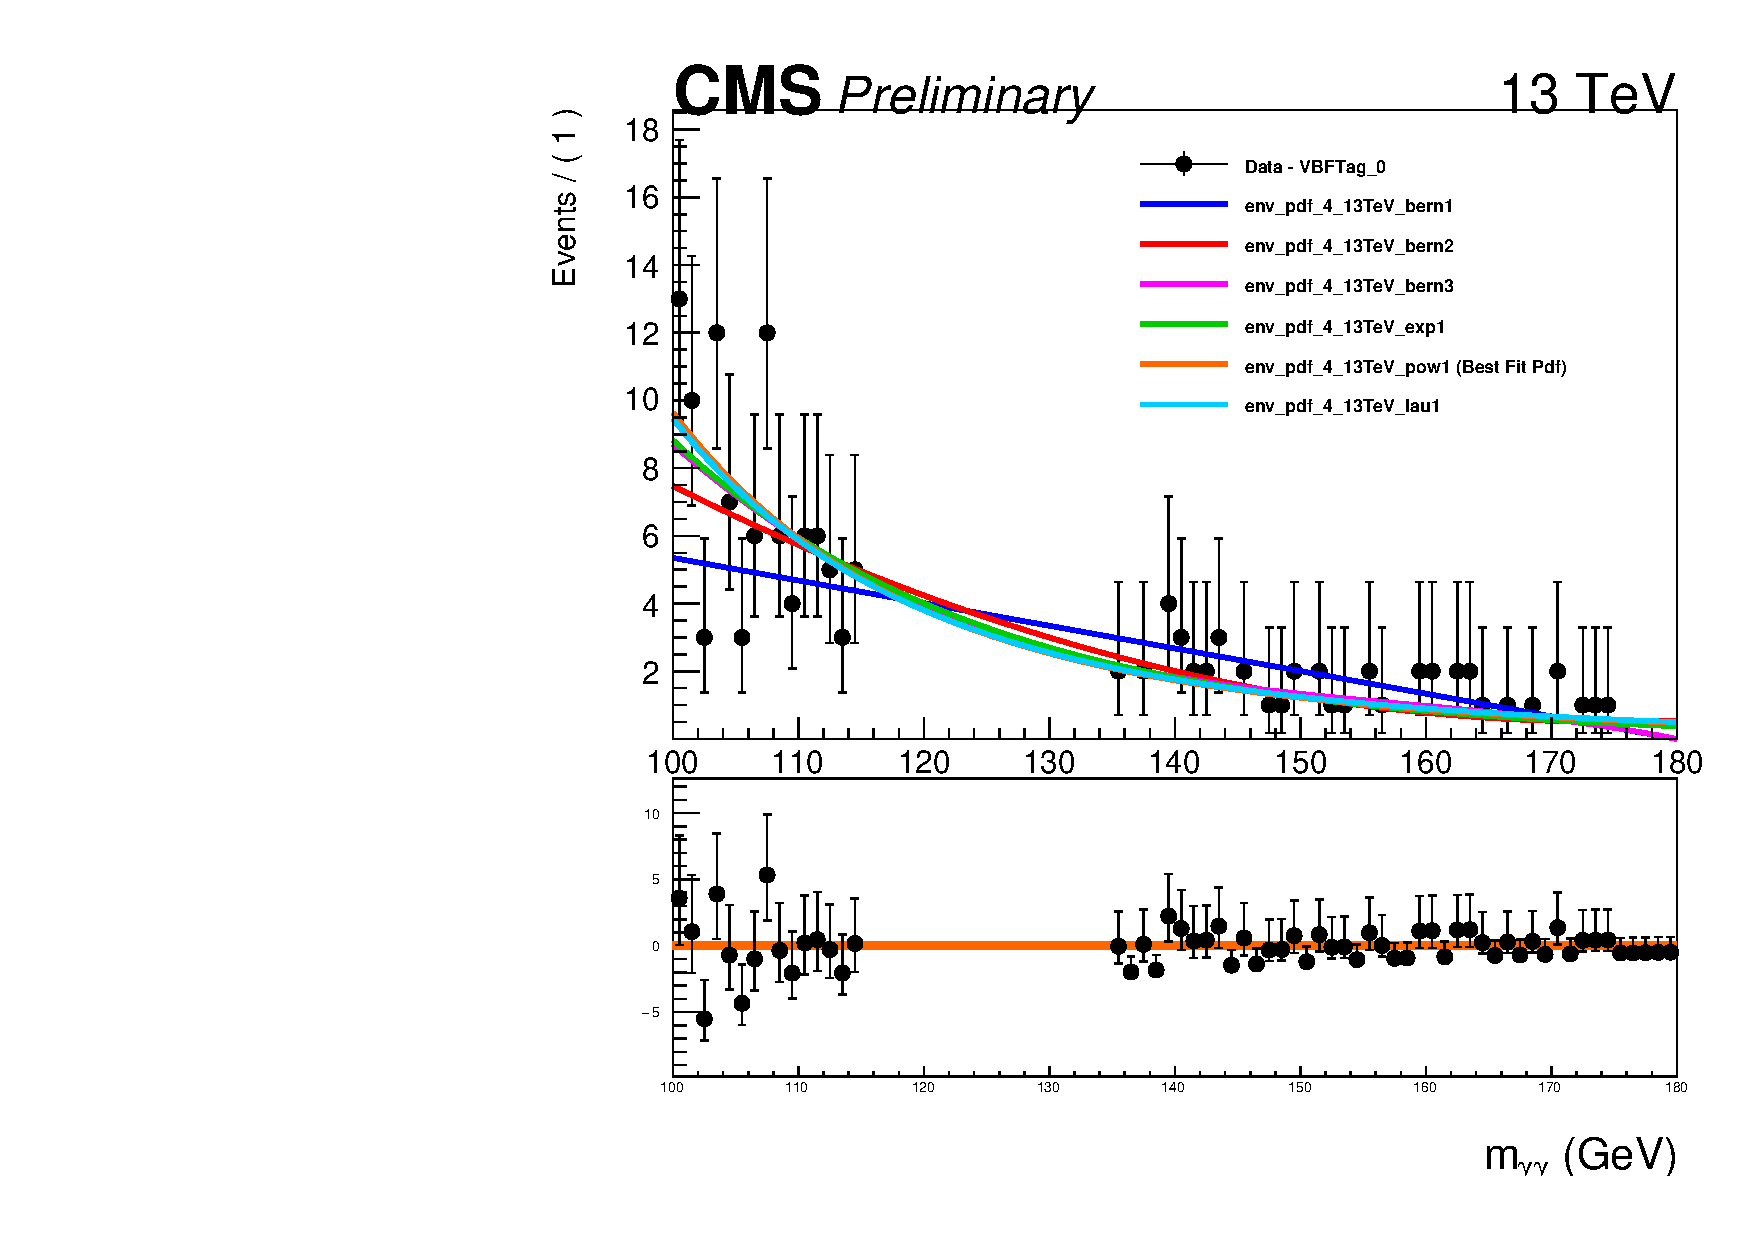
\includegraphics[width=0.48\textwidth]{modellingFigures/multipdf/multipdf_VBFTag_0.pdf}}
 \subfloat[\VBFTag 1]      {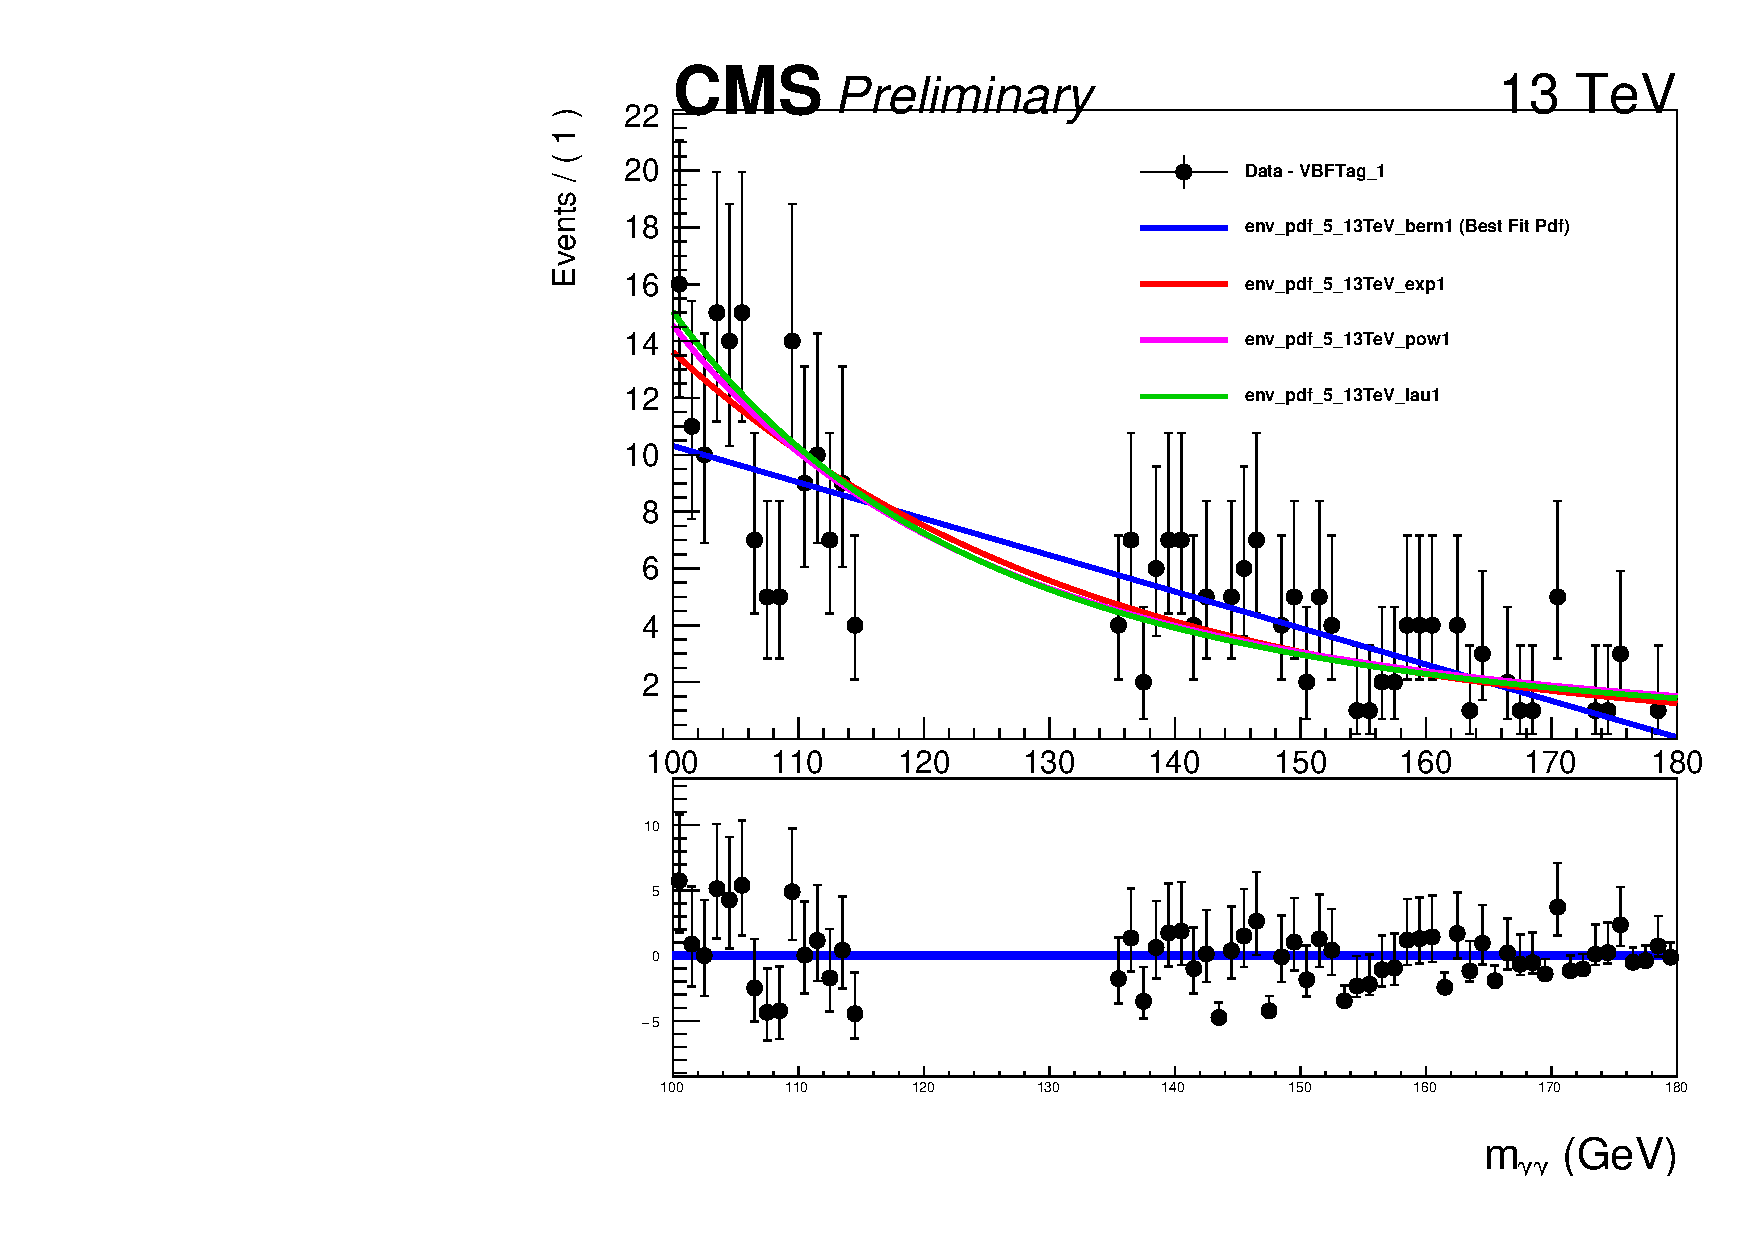
\includegraphics[width=0.48\textwidth]{modellingFigures/multipdf/multipdf_VBFTag_1.pdf}}\\
 \subfloat[\TTHLeptonicTag]{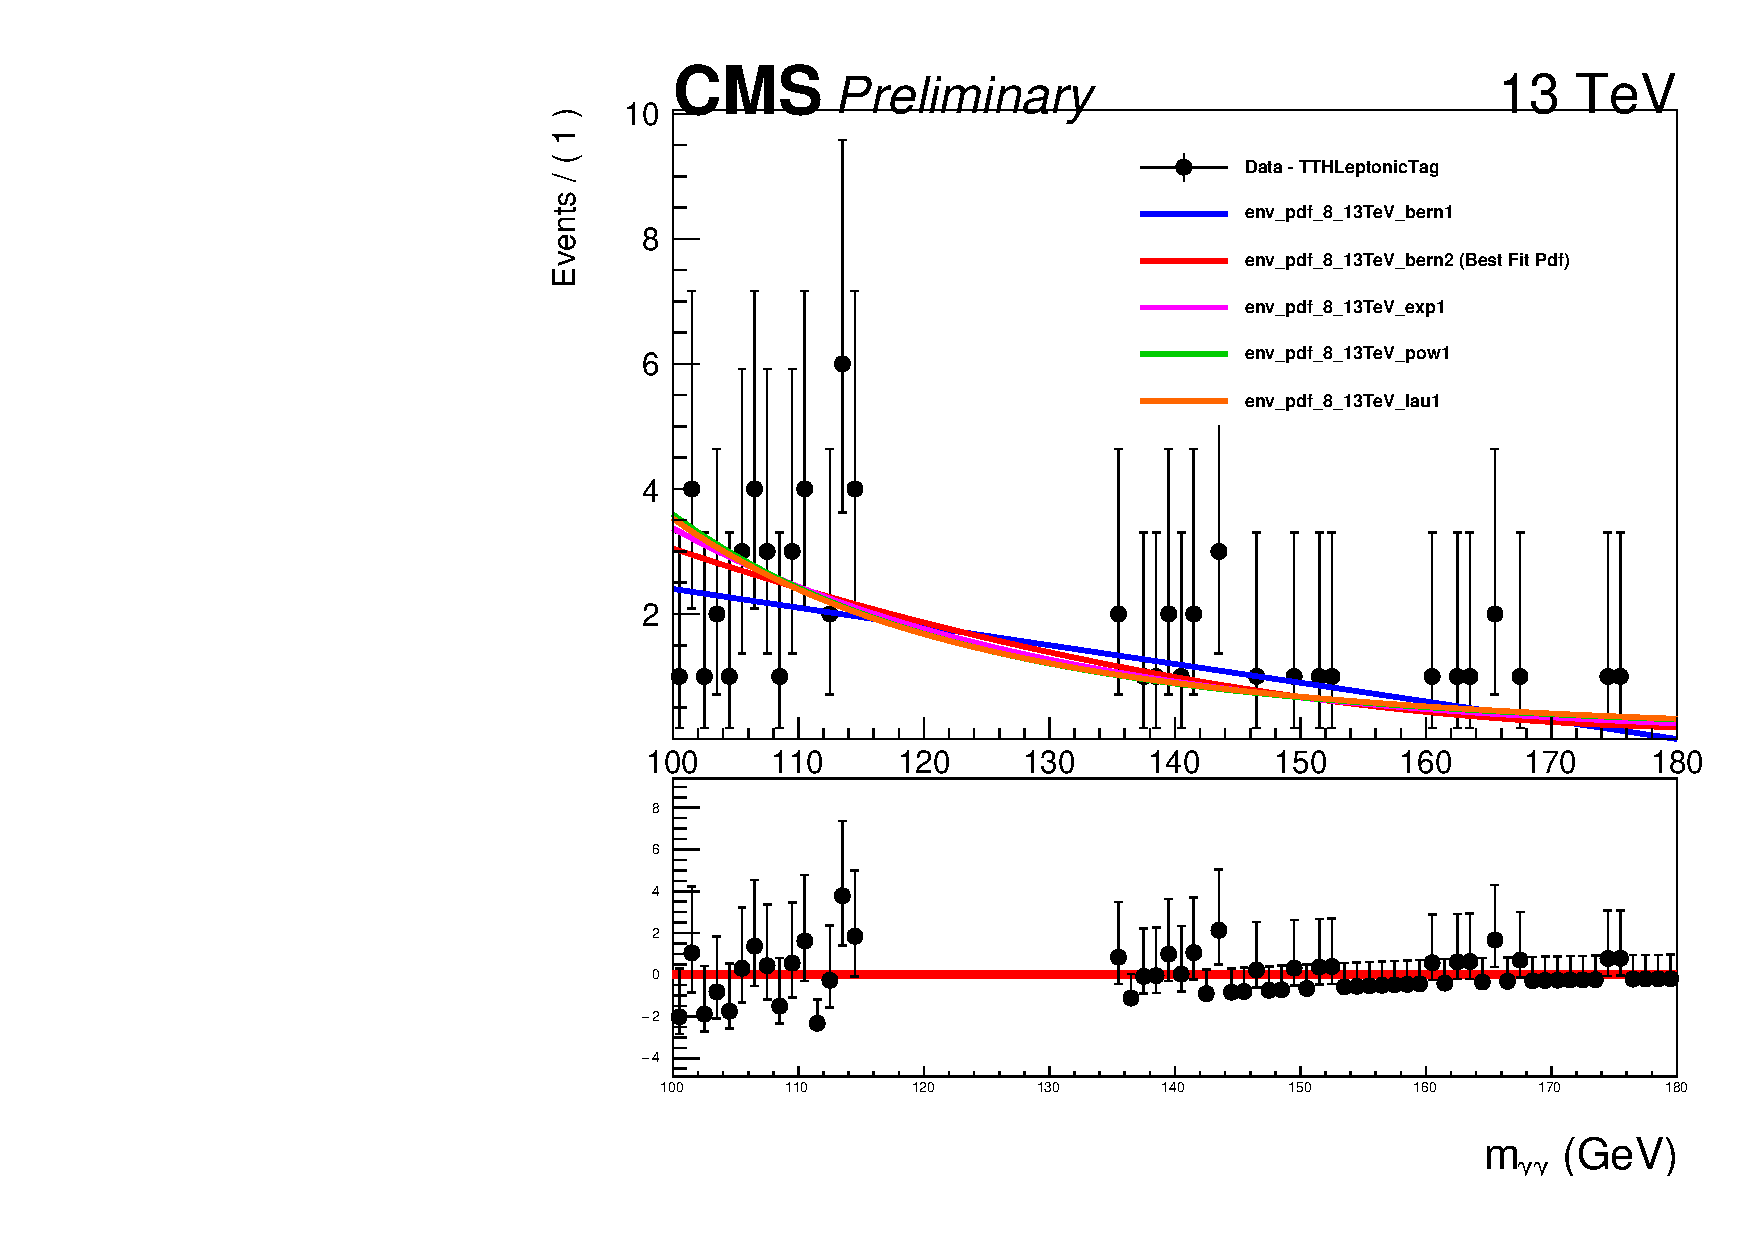
\includegraphics[width=0.48\textwidth]{modellingFigures/multipdf/multipdf_TTHLeptonicTag.pdf}}
 \subfloat[\TTHHadronicTag]{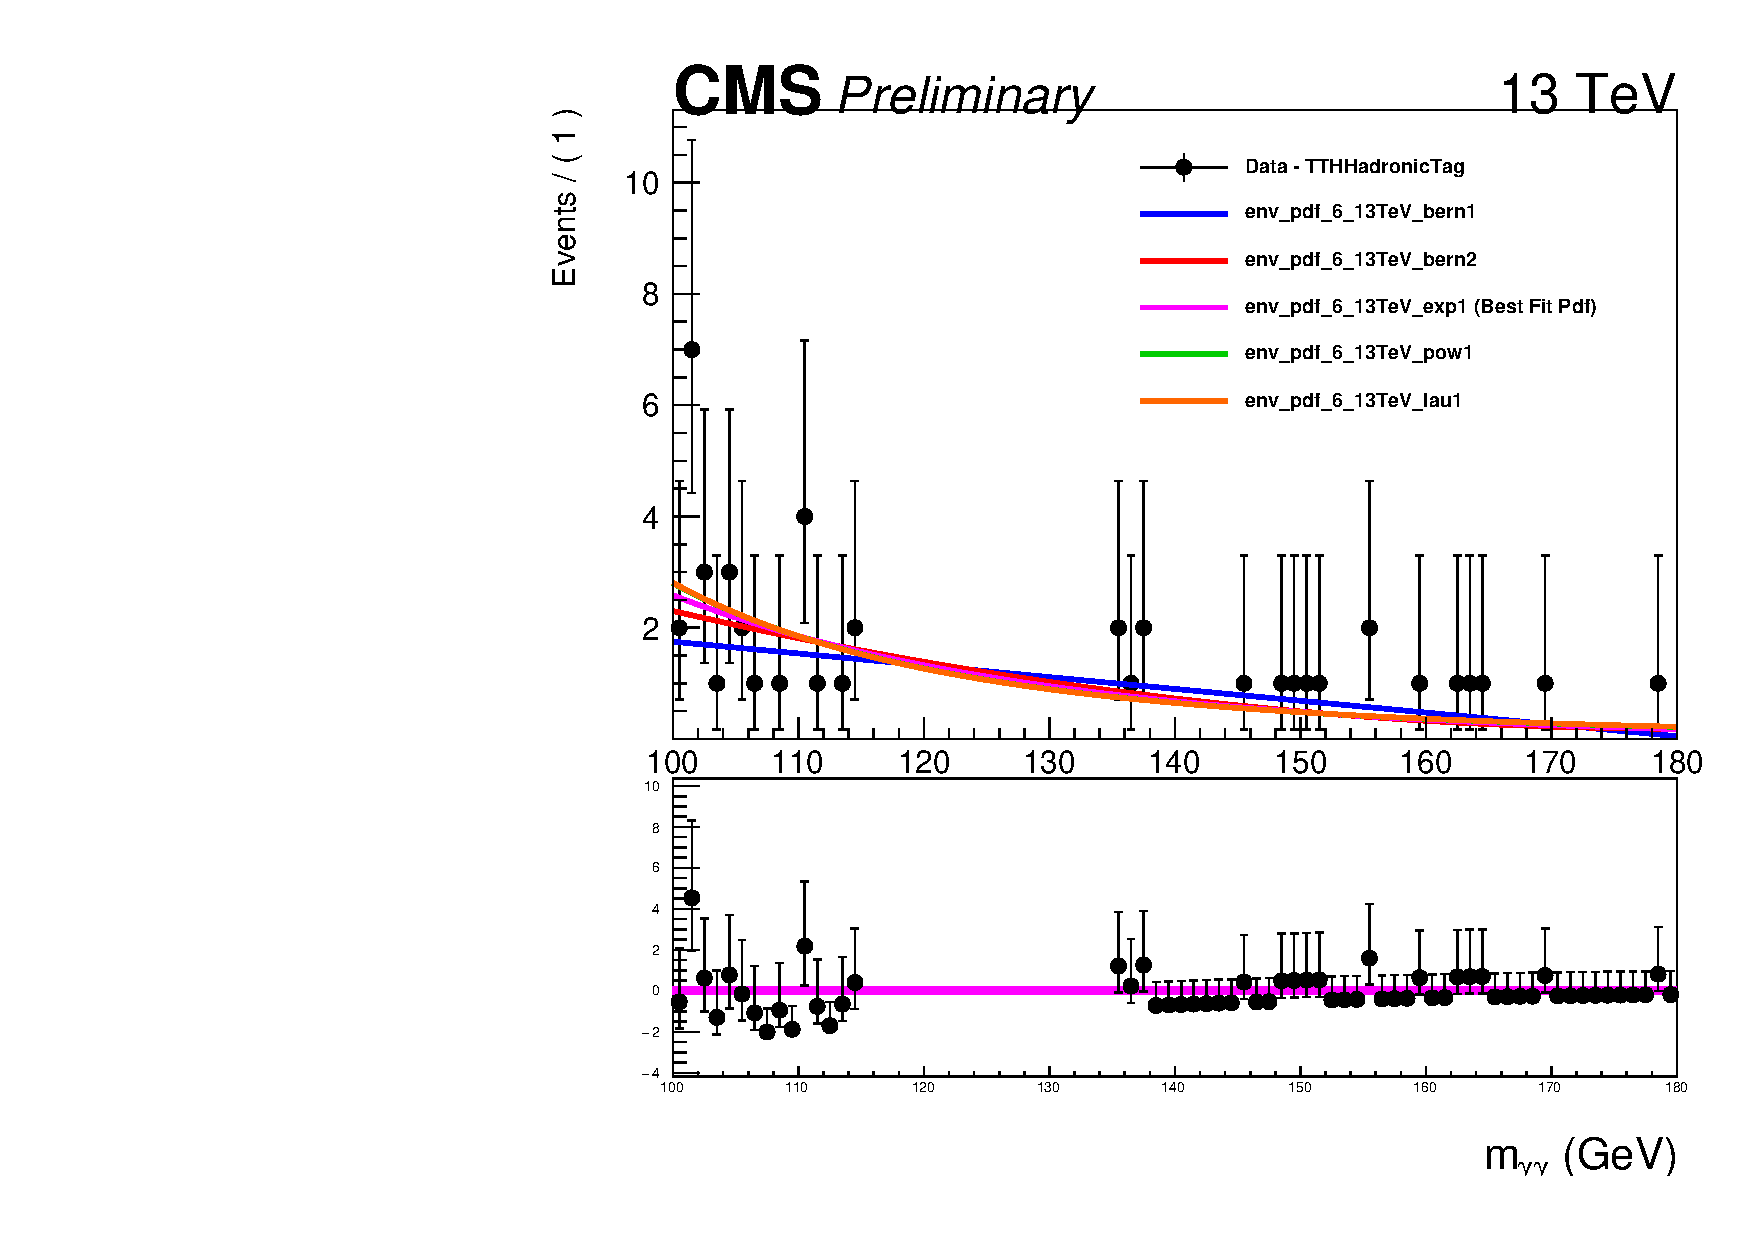
\includegraphics[width=0.48\textwidth]{modellingFigures/multipdf/multipdf_TTHHadronicTag.pdf}}\\
 \caption{The set of candidate functions chosen to parametrise the background using the discrete profiling method in the \VBFTag and \TTHTag categories.} 
 \label{fig:model:bkg_multipdf_exc}
 \end{center}
\end{figure}

The expected number of background events per $\GeV$ around $125\GeV$ is shown in \Table~\ref{tab:model:sig_bkg_yields} alongside the expected number of signal events for each category, which is broken down by the contribution of each production mode. The \effSigma (the width of the smallest widnow containing $68.3\%$ of the distribution) and $\sigma_{HM}$ (the width of the distribution at half of the maximum value, divided by $2.35$) are also shown. The expected number of background events is quoted for a $\pm 1 \effSigma$ window around $125\GeV$, using the best-fit background function.

 \begin{table}
  \resizebox{\textwidth}{!}{
%%%%%%%%%%%%%%%%%%%%%%%%%%%%%%%%%%%%%%%%%%%%%%%%%%%%%%%
%\begin{tabular}{ |r | c | c | c  | c |  c |  c |  c |  c |  c | }
%\hline
%\multirow{2}{*}{Event Categories} &\multicolumn{8}{|l|}{SM 125GeV Higgs boson expected signal} & Average Bkg \\ \cline{2-9}
%  &  Total & ggh (\%) & vbf (\%) & wh (\%)  & zh (\%) & tth (\%)  &   $\sigma_{\text{eff}} $  & $\sigma_{\text{HM}} $ & (GeV$^{-1}$) \\
%  \hline
%  Untagged Tag 0 &    11.92  &  79.10  &  7.60  &  7.11  &  3.59  &  2.60 & 1.18 & 1.03 & 4.98 \\
%  Untagged Tag 1 &    128.78  &  85.98  &  7.38  &  3.70  &  2.12  &  0.82 & 1.35 & 1.20 & 199.14 \\
%  Untagged Tag 2 &    220.12  &  91.11  &  5.01  &  2.18  &  1.23  &  0.47 & 1.70 & 1.47 & 670.44 \\
%  Untagged Tag 3 &    258.50  &  92.35  &  4.23  &  1.89  &  1.06  &  0.47 & 2.44 & 2.17 & 1861.23 \\
%  VBF Tag 0 &    9.35  &  29.47  &  69.97  &  0.29  &  0.07  &  0.20 & 1.60 & 1.33 & 3.09 \\
%  VBF Tag 1 &    15.55  &  44.91  &  53.50  &  0.86  &  0.38  &  0.35 & 1.71 & 1.40 & 22.22 \\
%  TTH Hadronic Tag &    2.42  &  16.78  &  1.28  &  2.52  &  2.39  &  77.02 & 1.39 & 1.21 & 1.12 \\
%  TTH Leptonic Tag &    1.12  &  1.09  &  0.08  &  2.43  &  1.06  &  95.34 & 1.61 & 1.35 & 0.42 \\
%  Total &    647.77  &  87.93  &  7.29  &  2.40  &  1.35  &  1.03 & 1.88 & 1.52 & 2762.65 \\
%  \hline
%  \end{tabular}
  %%%%%%%%%%%%%%%%%%%%%%%%%%%%%%%%%%%%%%%%%%%%%%%%%%%%%%%
  %%%%%%%%%%%%%%%%%%%%%%%%%%%%%%%%%%%%%%%%%%%%%%%%%%%%%%%
  \begin{tabular}{ |r | c | c | c  | c |  c |  c |  c |  c |  c | }
  \hline
  \hline
  \hline
  \multirow{2}{*}{Event Categories} &\multicolumn{8}{|l|}{SM 125GeV Higgs boson expected signal} & Bkg Events\\ \cline{2-9}
    &  Total & ggh (\%) & vbf (\%) & wh (\%) & zh (\%) & tth (\%) &   $\sigma_{\text{eff}} $  & $\sigma_{\text{HM}} $ & in $ \pm \sigma_{eff}$  \\
    \hline
    \hline
    Untagged Tag 0 &    45.69  &  81.41  &  11.25  &  3.60  &  1.78  &  1.96 & 1.26 & 1.14 & 53.98 \\
    Untagged Tag 1 &    495.36  &  88.60  &  7.36  &  2.23  &  1.27  &  0.54 & 1.44 & 1.27 & 2630.66 \\
    Untagged Tag 2 &    661.79  &  91.23  &  5.50  &  1.83  &  1.04  &  0.40 & 1.96 & 1.68 & 9231.93 \\
    Untagged Tag 3 &    579.27  &  92.33  &  4.45  &  1.76  &  0.98  &  0.48 & 2.65 & 2.34 & 25503.31 \\
    VBF Tag 0 &    10.05  &  21.51  &  77.84  &  0.24  &  0.00  &  0.40 & 1.50 & 1.32 & 5.74 \\
    VBF Tag 1 &    12.31  &  36.48  &  62.50  &  0.38  &  0.16  &  0.48 & 1.62 & 1.33 & 23.05 \\
    VBF Tag 2 &    28.66  &  50.93  &  47.33  &  0.75  &  0.32  &  0.67 & 1.57 & 1.32 & 86.01 \\
    TTH Hadronic Tag &    5.38  &  11.36  &  0.81  &  0.73  &  2.12  &  84.98 & 1.42 & 1.29 & 6.64 \\
    TTH Leptonic Tag &    3.46  &  2.08  &  0.05  &  1.67  &  1.24  &  94.96 & 1.57 & 1.28 & 5.08 \\
    VH Met Tag &    10.84  &  46.42  &  3.36  &  19.47  &  21.73  &  9.02 & 1.78 & 1.51 & 72.96 \\
    VH LeptonicLoose Tag &    2.74  &  9.13  &  2.83  &  65.63  &  19.84  &  2.57 & 1.77 & 1.47 & 13.25 \\
    VH Hadronic Tag &    9.58  &  57.98  &  3.92  &  21.31  &  13.00  &  3.80 & 1.44 & 1.32 & 21.06 \\
    ZH Leptonic Tag &    0.52  &  0.00  &  0.00  &  0.00  &  97.37  &  2.63 & 1.60 & 1.33 & 0.39 \\
    WH Leptonic Tag &    3.59  &  1.24  &  0.66  &  87.53  &  4.77  &  5.80 & 1.63 & 1.35 & 6.71 \\
    Total &    1869.23  &  88.14  &  7.15  &  2.38  &  1.33  &  1.00 & 1.96 & 1.59 & 32056.29 \\
    \hline
    \hline
    \end{tabular}
    %%%%%%%%%%%%%%%%%%%%%%%%%%%%%%%%%%%%%%%%%%%%%%%%%%%%%%%

}
 \caption{ The expected number of signal and background events per category. The \effSigma of the signal model is also provided as an estimate of the $m_{\gamma\gamma}$ resolution in that category. The expected number of background events is quoted per \GeV in a $\pm 1 \effSigma$ window around 125 \GeV.}
 \label{tab:model:sig_bkg_yields}
\end{table}

\section{Systematic uncertainties}
\label{model:sec:systematics}

The systematic uncertainty impacting the background model is handled directly by the discrete profiling method described above. The uncertainties which affect the signal model are more numerous, and are implemented differently depending on their effect on the signal model.

Systematic uncertainties which affect the shape of the \mgg distribution are built directly into the signal models described in \Sec~\ref{model:sec:signal_model}. Most systematics of this type impact individual photon energies, and therefore the invariant mass. The effect of the systematic variation is propagated to the mean, \effSigma and normalisation of the signal \mgg distribution for each category and signal process. Corresponding nuisance parameters are then inserted which can modify the normalisation, mean and width of the \DCBpG parametrisations. An exception is the nuisance corresponding to the vertex efficiency, which instead modifies the relative mixing fraction of the \RV and \WV components of the model. The nuisances parameters are then Gaussian-constrained and allowed to be profiled in the \NLL minimisation when making measurements of the parameters of interest. Nuisances of this type are referred to hereafter as \emph{shape nuisances}. 

Uncertainties on selection efficiencies typically do not affect the shape of the \mgg distribution, but do change the final event count (or \emph{yield}) of the signal model for each category. Uncertainties of this type are therefore implemented as nuisance parameters which impact the yield. Depending on the source of the systematic uncertainty, categories can be scaled differently, although all categories will simultaneously either increase or decrease. The corresponding nuisance parameters are profiled in the \NLL minimisation with a \lnN~\cite{1987lognormal} constraint, which cannot give rise to negative yields. Systematics of this type are referred to as \emph{yield nuisances}, which are either symmetric or asymmetric. In the symmetric case, the upward and downward variations of the uncertainty are the same size. In the asymmetric case, the upward and downward variations are of different sizes.

Finally, certain sources of systematic uncertainty affect the categorisation of events. In this case, the systematic variations can cause events to move from one event category to another, or altogether out of the acceptance of the analysis. These systematic uncertainties are implemented as nuisance parameters which change the relative yield of event categories, and are referred to as \emph{category migration nuisances}. They are implemented analogously to yield nuisances, except that the yield of certain categories will increase while the yield of others must decrease in turn. Furthermore, separate nuisances are implemented to account for different types of migration: for instance, between the individual \VBFTag categories on the one hand, and then between all \VBFTag and all \Untagged categories on the other.

\subsection{Theory uncertainties}

\subsubsection{Gluon fusion contamination of \VBFTag and \TTHTag categories}
The theoretical prediction for the jet multiplicity in gluon fusion events is unreliable in cases with large number of jets. This leads to the introduction of an uncertainty on the contamination of \ggH events in other analysis categories which use jets in their selections. 

For \VBFTag categories, the uncertainty is estimated using the Stewart-Tackmann procedure~\cite{StewartTackmann}. This results in a set of category migration nuisances: a migration between \VBFTag categories (at most $39\%$ on category yield) and a migration between \Untagged and \VBFTag categories (at most $10\%$ on category yield); %jetveto

For the \TTHTag categories, this uncertainty is modelled by three yield nuisances:
\begin{itemize}
\item shower modelling uncertainty, which is estimated by comparing the jet multiplicity in data and simulation for $\Ptop \APtop \rightarrow \text{jets}$ events, where the tops quarks both decay to leptons, leading to variations of the order of 45\% on the yield of the \TTHTag categories; 
\item gluon splitting modelling, which is estimated from the ratio of \crosssection\s of $\Ptop \Ptop \Pbottom \Pbottom$ and $\Ptop \Ptop +2\text{ jet}$ events in 13\TeV data;
\item an additional nuisance included due to the small size of the simulated samples used in these studies.
\end{itemize}

\subsubsection{\Hgg branching ratio}
The uncertainty on the \Hgg branching fraction is taken directly from the \LHCHXSWG recommendation~\cite{LHCHXSWGYR4}. It is implemented as a yield nuisance affecting all analysis categories, and the variation is of 2.08\% on the category yield.

\subsubsection{Parton Distribution Functions}

The uncertainty on signal process \crosssection\s due to \PDF uncertainties produces both an overall change in signal yield and category migrations.

One symmetric yield nuisance for each signal process is included, accounting for both \PDF and the strong force coupling constant (\alphaS) uncertainties. Each varies the category yields according to the corresponding uncertainty in the process \crosssection, as provided by the \LHCHXSWG recommendation~\cite{LHCHXSWGYR4}. Namely, the \ggH, \VBF, \WH, \ZH, and \ttH process \crosssection\s are scaled by 3.2\%, 2.1\%, 1.9\%, 1.6\% and 3.6\% respectively. 

The relative yield change is modelled using a series of category migration nuisances. The size of the variations is determined according to the PDF4LHC prescription~\cite{Demartin:2010er}, by re-weighting individual events according to the NNPDF30 \PDF set~\cite{Carrazza:2015aoa}. The effect of the variations is normalised by their effect on the overall yield, such that they represent only migrations. The procedure results in 60 uncorrelated symmetric migration nuisances. The largest migrations are of the order of 2\% of category yields, but are typically below 0.4\%.

\subsubsection{QCD scale}
The uncertainty on the scale of the \QCD interaction is parametrised in terms of the renormalisation ($\mu_{Renorm.}$) and factorisation ($\mu_{Fact.}$) scales. The asymmetric yield nuisances corresponding to variations of these parameters are taken direction from the \LHCHXSWG recommendations for \crosssection\s~\cite{LHCHXSWGYR4}. The size of the effect for the \ggH, \VBF, \WH, \ZH and \ttH processes is $+4.6\%/-6.7\%$, $+0.4\%/-0.3\%$, $+0.5\%/-0.7\%$, $+3.8\%/-3.0\%$ and $+5.8\%/-9.2\%$ respectively. Three additional asymmetric category migration nuisances are also included. The size of their effect is estimated at generator level, by varying the values of $\mu_{Renorm.}$ and $\mu_{Fact.}$ by factors of $2$ (upward variation ) or $0.5$ (downward variation). The three category migration nuisances correspond to varying $\mu_{Renorm.}$ up or down while keeping $\mu_{Fact.}$ constant ; varying $\mu_{Fact.}$ up or down while keeping $\mu_{Renorm.}$ constant ; and varying both $\mu_{Renorm.}$ and $\mu_{Fact.}$ up or down uniformly. In each case the migrations are found to be of the order of 5-10\% of the category yield.

\subsubsection{Strong force coupling constant}
The effect of the uncertainty on the value of \alphaS is modelled as described in the \PDF uncertainty section. The yield nuisances for the \PDF uncertainties also incorporate the uncertainty on \alphaS. Three additional asymmetric category migration nuisances are included, the effect of which is determined according to the PDF4LHC prescription~\cite{Demartin:2010er} normalised by the overall effect on the signal yield. The largest migrations are of the order of $3.7\%$ of the category yield. 

\subsubsection{Underlying event and parton shower}
The uncertainty on the \emph{underlying event} is introduced because different models exist to describe the interactions of quarks and gluons in \pp collisions, each giving different predictions. In particular, this affects the modelling of jets. This uncertainty is taken into account as a set of category migration nuisances. The sizes of the variations are obtained from dedicated simulated samples where the parameters of the generators have been tuned differently. The category migrations evaluated are between: \VBFTag 0 and \VBFTag 1 categories (of the order of 7\%); and all \VBFTag categories and all \Untagged categories (of the order of 9\%).

The \emph{parton shower} refers to the emission of \QCD radiation from partons during \pp collisions. As for the underlying event, an uncertainty is introduced because different models and generators give different predictions, in particular in the reconstruction of jets. The resulting uncertainty is modelled analogously to the underlying event uncertainty.  The category migrations evaluated are between: \VBFTag 0 and \VBFTag 1 categories (of the order of 7\%); and all \VBFTag categories and all \Untagged categories (of the order of 9\%).


\subsection{Photon energy uncertainties}

\subsubsection{Modelling of detector response in \Geant}
The imperfect modelling of electromagnetic showers in the detector simulation software \Geant is modelled with a shape nuisance, as it impacts the photon energy scale. The size of the variation was determined with a dedicated simulated sample where the parameters of shower modelling were modified, leading to a small uncertainty on the photon energy scale. The size of the effect is approximately 0.05\% on the mean of the \mgg distribution in each category.

\subsubsection{Modelling of the material budget}
The imperfect modelling of the amount of material between the vertex and the \ECAL affects the simulation of the photon and electron showers. The uncertainty related to this effect is estimated with dedicated samples there the amount of simulated material is uniformly varied by $\pm 5\%$. It is treated as two separate shape nuisances, for \EB and \EE photons separately, which affect the mean of the \mgg distribution by at most 0.1\% (0.03\%) and the \effSigma by at most 3.5\% (7.6\%) for the \EB (\EE) photons.

\subsubsection{Non-linearity of detector response}
The uncertainty associated with the fact that the \ECAL response is not linear is estimated by comparing boosted \Zee decays in data and simulation. Individual photon energies are affected by up to 0.2\%. The effect is propagated as a shape nuisance, which varies the mean of the \mgg distribution by 0.1\% in each category.

\subsubsection{Non-uniformity of the light collection}
The uncertainty on the response of the \ECAL crystals depending on their position in \eta is modelled separately as shape nuisances for photons in the barrel and in the endcaps. The size of the uncertainty is 0.07\% on the photon energies. The effect is propagated to the \mgg distribution of each category and applied as separate shape nuisances in the \EE and \EB, which vary the mean by up to 0.2\% and the \effSigma by up to 5\%.

\subsubsection{Per-photon energy resolution}
The uncertainty of the per-photon energy resolution is conservatively evaluated by scaling the output of the \PhoEnergyBdt described in \Sec~\ref{sec:reco:photon:phoenergybdt} by $\pm5\%$. This uncertainty is propagated throughout the analysis and modelled as a yield nuisance. The size of the variation is at most 3\% depending on the analysis category.

\subsubsection{Photon energy scale and resolution}
After the calibration of the \ECAL described in \Sec~\ref{sec:cms:ecal:calibration}, there are still some discrepancies in the photon energy scale and resolution between simulation and data. Since electrons and photons are both reconstructed as \SC\s, these discrepancies can be studied using \Zee events where the electrons are reconstructed as photons.
For \SC\s in eight \RNINE and $|\eta|$ classes, the invariant mass distributions in data and simulation are both fitted with a Breit-Wigner (which models the natural shape of the \PZ-peak) convoluted with a \CB function (which describes the \ECAL resolution and losses due to unrecovered energy from bremsstrahlung). The natural width and pole mass of the $\PZ$ boson are fixed to their accepted values~\cite{PDGBooklet} in this parametrisation. 

The corrections to the photon energy scale are given by the relative differences between the best-fit means of the \CB in data and simulation, divided by the $\PZ$ boson pole mass, in each bin. The corrections to the photon energy resolution are applied by adding additional smearing terms to the width of the \CB in quadrature. The additional scale and resolution corrections described above each have uncertainties, which are related to choices made for the \Zee event selection and classification, as well as the difference between the final electron and photon energy regression \BDT\s. The uncertainties on the energy scale and resolution are quantified for each photon class, and propagated to the \mgg distribution in each analysis category. This results in a shape nuisance for the photon energy scale in four classes (high and low \RNINE, each for \EB and \EE), and eight shape nuisances for the photon energy smearing (as for the photon energy scale, but parametrised also as constant and stochastic contributions). 

The size of the systematic uncertainties are of the order of 0.15\% to 0.5\% depending on the photon class. The effect on the mean of the \mgg distribution is at most 0.25\%, while the effect on the \effSigma is at most 20\%, depending on the analysis category.

\subsubsection{Preselection}
The efficiency of the photon preselection is quantified using the \TagAndProbe method described in \Sec~\ref{reco:sec:pho:preselection}, which also provides systematic uncertainties for different photon classes. The systematic uncertainties are propagated to a yield nuisance,
the effect of which is around 4\% on the category yields.

\subsubsection{Shower shape corrections}
The uncertainty deriving from the imperfect modelling of shower shape variables is estimated using simulated samples with and without the corrections. This effect is of order 0.064\% on the photon energy scale, and is implemented as four shape nuisances for photons in different $\eta$ and \RNINE classes, which vary the \mgg distribution mean by at most 0.2\% and \effSigma by at most 1.8\%.

\subsection{Per-event uncertainties}

\subsubsection{Integrated luminosity}
The uncertainty on the value of the integrated luminosity of the data sample is modelled as a scale nuisance, the size of which is 6.2\% on the yield of all signal processes. 

\subsubsection{Jet energy scale and resolution}
The uncertainties on the jet energy scale are described by migrations nuisances: between \VBFTag 0 and \VBFTag 1 (at most 13.6\% on the category yield); between all \VBF and \Untagged categories (at most 12\%) ; and between \TTHTag and \Untagged categories (at most 15\%).

The nuisances for the jet energy resolution are treated analogously, with migrations of at most 2.2\% between \VBFTag 0 and \VBFTag 1 categories; at most 2.9\% between \VBF and \Untagged categories ; and at most 12.8\% between \TTHTag and \Untagged categories.

\subsubsection{Lepton reconstruction and $\Pbottom$-tagging efficiencies}
The uncertainty on the reconstruction of electrons and muons is determined by considering the ration of leptons reconstructed in data and simulation. The result is implemented as a yield uncertainty for the \TTHTag categories of the order of 1\%.

Similarly, the uncertainty on the tagging of $\Pbottom$ jets is evaluated by varying the ratio between the measured $\Pbottom$-tagging efficiency in data and simulation within their uncertainty. This is propagated to a yield nuisance, which has an effect of the order of 2\% for \TTHTag categories.

\subsubsection{Rejection of jets from \PU}
The uncertainty on \PU jet rejection using the selection of the \RMS (as described in \Sec~\ref{reco:sec:jets}) is described by a migrations nuisances between all \VBF and \Untagged categories (at most 3.5\%).

A further uncertainty, relating to the number of \PU jets in simulation which are reconstructed as genuine jets from the hard scatter, is described by migrations nuisances: between \VBFTag 0 and \VBFTag 1 (at most 1.2\% on the category yield); and between all \VBF and \Untagged categories (at most 1.3\%).

\subsubsection{Trigger efficiency}
The uncertainty on the trigger efficiency is estimated using a \TagAndProbe method as described in \Sec~\ref{sec:reco:data}. The uncertainty is applied as a yield nuisance parameter of size 0.1\%.

\subsubsection{Vertex-finding efficiency}
The uncertainty on the vertex-finding efficiency is determined by comparing the fraction of correctly identified vertices in \Zmumu between data and simulation. The uncertainty is modelled as a shape nuisance which alters the \RV/\WV mixing fraction of each signal model. The variation is of the order of 1.5\% on the \RV fraction.

